%===============================================================================
% LaTeX sjabloon voor de bachelorproef toegepaste informatica aan HOGENT
% Meer info op https://github.com/HoGentTIN/latex-hogent-report
%===============================================================================

\documentclass[dutch,dit,thesis]{hogentreport}

% - If necessary, replace the option `dit`' with your own department!
%   Valid entries are dbo, dbt, dgz, dit, dlo, dog, dsa, soa
% - If you write your thesis in English (remark: only possible after getting
%   explicit approval!), remove the option "dutch," or replace with "english".

\usepackage{lipsum} % For blind text, can be removed after adding actual content
\usepackage{biblatex}
\usepackage{glossaries}

\makeglossaries



\newacronym{MDD}{MDD}{Model Driven Development}
\newacronym{MDA}{MDA}{Model Driven Architecture}
\newacronym{xUML}{xUML}{executable Unified Modeling Language}
\newacronym{UML}{UML}{Unified Modeling Language}
\newacronym{CASE}{CASE}{Computer Aided Software Engineering}
\newacronym{PWA}{PWA}{Progressieve Webapp}
\newacronym{UX}{UX}{User Experience (gebruikerservaring)}
\newacronym{API}{API}{Application Programming Interface}
\newacronym{AI}{AI}{Artificiële intelligentie}
\newacronym{ML}{ML}{Machine Learning}
\newacronym{MBE}{MBE}{Model-Based Engineering}
\newacronym{DEMO}{DEMO}{Design and Engineering Methodology for Organizations}
\newacronym{FOD MOB}{FOD MOB}{Federale Overheidsdienst Mobiliteit}
\newacronym{FCP}{FCP}{First Contentful Paint}
\newacronym{LCP}{LCP}{Largest Contentful Paint}
\newacronym{TBT}{TBT}{Total Blocking Time}
\newacronym{CLS}{CLS}{Cumulative Layout Shift}


%\usepackage{minted}
\captionsetup[table]{justification=centering, singlelinecheck=false}  % Verticaal centreren van caption bij tabellen


%% Pictures to include in the text can be put in the graphics/ folder
\graphicspath{{../graphics/}}

%% For source code highlighting, requires pygments to be installed
%% Compile with the -shell-escape flag!
%% \usepackage[chapter]{minted}
%% If you compile with the make_thesis.{bat,sh} script, use the following
%% import instead:
\usepackage{minted}  % No extra options needed
\usemintedstyle{solarized-light}  % Load the preferred style
\usepackage{float}

%% Formatting for minted environments.
\setminted{%
    autogobble,
    frame=lines,
    breaklines,
    linenos,
    tabsize=4
}

%% Ensure the list of listings is in the table of contents
\renewcommand\listoflistingscaption{%
    \IfLanguageName{dutch}{Lijst van codefragmenten}{List of listings}
}
\renewcommand*\listoflistings{%
    \cleardoublepage\phantomsection\addcontentsline{toc}{chapter}{\listoflistingscaption}%
    \listof{listing}{\listoflistingscaption}%
}


% Other packages not already included can be imported here

%%---------- Document metadata -------------------------------------------------

\author{Senne Timbreur}
\supervisor{Mevr. F. Spriet}
\cosupervisor{Mevr. J. Alexander}
\title[Optionele ondertitel]%
{Grenzen van de low-code tool Mendix}
\academicyear{\advance\year by -1 \the\year--\advance\year by 1 \the\year}
\examperiod{2}
\degreesought{\IfLanguageName{dutch}{Professionele bachelor in de toegepaste informatica}{Bachelor of applied computer science}}
\partialthesis{false} %% To display 'in partial fulfilment'
%\institution{Internshipcompany BVBA.}

%% Add global exceptions to the hyphenation here
\hyphenation{back-slash}

%% The bibliography (style and settings are  found in hogentthesis.cls)
\addbibresource{bachproef.bib}            %% Bibliography file
\addbibresource{../voorstel/voorstel.bib} %% Bibliography research proposal
\defbibheading{bibempty}{}

%% Prevent empty pages for right-handed chapter starts in twoside mode
\renewcommand{\cleardoublepage}{\clearpage}

\renewcommand{\arraystretch}{1.2}

%% Content starts here.
\begin{document}
    
    %---------- Front matter -------------------------------------------------------
    
    \frontmatter
    
    \hypersetup{pageanchor=false} %% Disable page numbering references
    %% Render a Dutch outer title page if the main language is English
    \IfLanguageName{english}{%
        %% If necessary, information can be changed here
        \degreesought{Professionele Bachelor toegepaste informatica}%
        \begin{otherlanguage}{dutch}%
            \maketitle%
        \end{otherlanguage}%
    }{}
    
    %% Generates title page content
    \maketitle
    \hypersetup{pageanchor=true}
    
    %%=============================================================================
%% Voorwoord
%%=============================================================================

\chapter{\IfLanguageName{dutch}{Woord vooraf}{Preface}}%
\label{ch:voorwoord}

Deze bachelorproef liep parallel met mijn stage, waar ik voor het eerst in contact kwam met low-code ontwikkeling. Tijdens deze stage kreeg ik de kans om de technologie in de praktijk toe te passen en leerde ik de voordelen ervan kennen, zoals snelle ontwikkeling en visuele modellering. Wat begon als een nieuwe manier van werken, groeide al snel uit tot een onderwerp dat mijn interesse wekte.

Via deze bachelorproef kreeg ik de mogelijkheid om low-code niet enkel praktisch toe te passen, maar ook inhoudelijk en kritisch te onderzoeken. Ik ging dieper in op de technologische en organisatorische afwegingen die bij low-code komen kijken, en ontdekte hoe complex de besluitvorming rond technologie in realiteit kan zijn.

Ik wil graag enkele mensen bedanken die een belangrijke rol gespeeld hebben in dit proces. Bart Claeys en Jodie Alexander van apvine wil ik bedanken voor hun ondersteuning en de inzichten die ze met me deelden. Lieven Debusscher van \gls{FOD MOB} ben ik erkentelijk voor zijn bereidheid om bij te dragen aan het onderzoek en zijn waardevolle perspectieven. Tot slot gaat mijn oprechte dank uit naar mijn promotor Fien Spriet van HOGENT, voor haar begeleiding, feedback en steun gedurende dit hele traject.

Deze bachelorproef was niet enkel een academisch project, maar ook een kans om praktijk en theorie met elkaar te verbinden. Een ervaring waar ik met veel voldoening op terugkijk.



    %%=============================================================================
%% Samenvatting
%%=============================================================================

% TODO: De "abstract" of samenvatting is een kernachtige (~ 1 blz. voor een
% thesis) synthese van het document.
%
% Een goede abstract biedt een kernachtig antwoord op volgende vragen:
%
% 1. Waarover gaat de bachelorproef?
% 2. Waarom heb je er over geschreven?
% 3. Hoe heb je het onderzoek uitgevoerd?
% 4. Wat waren de resultaten? Wat blijkt uit je onderzoek?
% 5. Wat betekenen je resultaten? Wat is de relevantie voor het werkveld?
%
% Daarom bestaat een abstract uit volgende componenten:
%
% - inleiding + kaderen thema
% - probleemstelling
% - (centrale) onderzoeksvraag
% - onderzoeksdoelstelling
% - methodologie
% - resultaten (beperk tot de belangrijkste, relevant voor de onderzoeksvraag)
% - conclusies, aanbevelingen, beperkingen
%
% LET OP! Een samenvatting is GEEN voorwoord!

%%---------- Nederlandse samenvatting -----------------------------------------
%
% TODO: Als je je bachelorproef in het Engels schrijft, moet je eerst een
% Nederlandse samenvatting invoegen. Haal daarvoor onderstaande code uit
% commentaar.
% Wie zijn bachelorproef in het Nederlands schrijft, kan dit negeren, de inhoud
% wordt niet in het document ingevoegd.

\IfLanguageName{english}{%
\selectlanguage{dutch}
\chapter*{Samenvatting}
\lipsum[1-4]
\selectlanguage{english}
}{}

%%---------- Samenvatting -----------------------------------------------------
% De samenvatting in de hoofdtaal van het document

\chapter{\IfLanguageName{dutch}{Samenvatting}{Abstract}}
\label{ch:samenvatting}


Deze bachelorproef onderzoekt de grenzen van het low-codeplatform Mendix bij het ontwikkelen van zakelijke applicaties, en gaat na in welke situaties high- codeontwikkeling een meer geschikte keuze vormt. De aanleiding voor dit onderzoek ontstond tijdens mijn stage, waar ik voor het eerst in aanraking kwam met Mendix en low-code in het algemeen. Via deze bachelorproef kreeg ik de kans om deze technologie niet enkel praktisch te ervaren, maar ook grondiger te analyseren binnen een bredere organisatorische en technologische context.

Low-codeontwikkeling biedt heel wat voordelen, zoals een versnelde oplevering, visuele modellering en een hogere toegankelijkheid voor gebruikers zonder technische achtergrond. In de praktijk blijkt echter dat Mendix, hoewel het platform over veel mogelijkheden beschikt, ook beperkingen kent bij projecten die complex zijn of een hoge graad van maatwerk vereisen. Vanuit deze vaststelling werd de centrale onderzoeksvraag geformuleerd: \textit{Wat zijn de grenzen van de low-code-tool Mendix bij het ontwikkelen van zakelijke applicaties, en wanneer is high-code-ontwikkeling meer geschikt?}

Om deze vraag te beantwoorden, werd een kwalitatieve onderzoeksaanpak gehanteerd. Deze bestond enerzijds uit interviews met beslissingsmakers bij \gls{FOD MOB}, een organisatie met een intern Java-team die frequent samenwerkt met low-codepartner apvine. Anderzijds werd een analyse uitgevoerd van historische projectdocumentatie om te identificeren waar de technologiekeuze tot frictie of herziening leidde. Daarnaast werd er ook praktisch onderzoek uitgevoerd, waarbij een vergelijkbare toepassing zowel in Mendix als in high-code (JavaScript/React) werd gebouwd. Deze hands-on vergelijking maakte het mogelijk om niet alleen theoretisch, maar ook functioneel inzicht te verwerven in de mogelijkheden en beperkingen van beide benaderingen.

Uit de analyse blijkt dat Mendix bijzonder krachtig is voor standaard bedrijfsprocessen, prototypes en projecten met strakke deadlines. De tool botst echter op beperkingen wanneer er nood is aan geavanceerde integraties, uitgebreide businesslogica of een hoge mate van technische controle.
Bovendien werd vastgesteld dat het gebrek aan een formeel beslissingskader binnen projectteams kan leiden tot suboptimale keuzes.

De bachelorproef concludeert dat het opstellen van een transparant en gestructureerd beslissingskader, waarin zowel technische als organisatorische factoren worden meegenomen, cruciaal is. Zo’n kader kan dienen als leidraad bij het maken van weloverwogen technologiekeuzes. Door het beslissingsproces te structureren en te onderbouwen, wordt niet alleen de efficiëntie van projecten bevorderd, maar ook de kwaliteit en het draagvlak van de gekozen oplossingen binnen IT-omgevingen versterkt.




    
    %---------- Inhoud, lijst figuren, ... -----------------------------------------
    
    \tableofcontents
    
    % In a list of figures, the complete caption will be included. To prevent this,
    % ALWAYS add a short description in the caption!
    %
    %  \caption[short description]{elaborate description}
    %
    % If you do, only the short description will be used in the list of figures
    
    \listoffigures
    
    % If you included tables and/or source code listings, uncomment the appropriate
    % lines.
    \listoftables
    
    \cleardoublepage
    \phantomsection
    \addcontentsline{toc}{chapter}{Lijst van afkortingen}
    \printglossary[type=\acronymtype, title={Lijst van afkortingen}]
    
    
    % Als je een lijst van afkortingen of termen wil toevoegen, dan hoort die
    % hier thuis. Gebruik bijvoorbeeld de ``glossaries'' package.
    % https://www.overleaf.com/learn/latex/Glossaries
    
    %---------- Kern ---------------------------------------------------------------
    
    \mainmatter{}
    
    % De eerste hoofdstukken van een bachelorproef zijn meestal een inleiding op
    % het onderwerp, literatuurstudie en verantwoording methodologie.
    % Aarzel niet om een meer beschrijvende titel aan deze hoofdstukken te geven of
    % om bijvoorbeeld de inleiding en/of stand van zaken over meerdere hoofdstukken
    % te verspreiden!
    
    %%=============================================================================
%% Inleiding
%%=============================================================================

\chapter{\IfLanguageName{dutch}{Inleiding}{Introduction}}%
\label{ch:inleiding}

Apvine, een toonaangevend IT-consultancybedrijf, maakt intensief gebruik van het low-code platform Mendix om zakelijke applicaties snel en efficiënt te ontwikkelen. Deze aanpak verlaagt de ontwikkeltijd en biedt een flexibele oplossing voor veel projecten. Alleen wanneer applicaties complexe bedrijfslogica, real-time gegevensverwerking of integraties met legacy-systemen vereisen, kunnen de beperkingen van low-code ontwikkeling zichtbaar worden.

In zulke gevallen kan een hybride of high-code aanpak nodig zijn, maar zonder een duidelijk beslissingskader is het lastig om te bepalen wanneer deze overstap gemaakt moet worden. Dit gebrek aan richtlijnen kan leiden tot projectvertragingen, hogere kosten en onverwachte aanpassingen. Dit kan een negatieve impact hebben op zowel apvine als haar klanten.

Dit onderzoek richt zich op het vaststellen van de grenzen van Mendix en het ontwikkelen van een gestructureerd beslissingskader, zodat projectmanagers en softwarearchitecten beter onderbouwde keuzes kunnen maken tussen low-code en high-code ontwikkeling.

\section{Kadering begrippen}
Voorafgaand aan de uitwerking van deze bachelorproef is het belangrijk om enkele kernbegrippen te kaderen. Door vooraf duidelijk te omschrijven wat we precies verstaan onder termen zoals low-code en high-code, zorgen we ervoor dat alle lezers met dezelfde basiskennis starten. Dit voorkomt verwarring en maakt de verdere analyse en besluitvorming beter te volgen en te interpreteren.
\subsection{High-code}
High-code, ook wel traditionele softwareontwikkeling genoemd, houdt in dat applicaties volledig worden geprogrammeerd met behulp van programmeertalen zoals Java, C\#, Python, JavaScript, ... . Deze aanpak biedt maximale controle, technische diepgang en flexibiliteit. Dit maakt het mogelijk om robuuste, schaalbare en volledig op maat gemaakte oplossingen te bouwen. High-code is bij uitstek geschikt voor toepassingen met complexe bedrijfslogica, uitgebreide integraties, hoge prestaties of specifieke beveiligingseisen. Hoewel het meer tijd en gespecialiseerde kennis vereist dan low-code, levert het doorgaans beter onderhoudbare en diep geïntegreerde software op
\textcite{Northcutt2023}.
\subsection{Low-code}
Low-code is een methode van softwareontwikkeling waarbij applicaties voornamelijk worden gebouwd via visuele interfaces, met gebruik van drag-and-drop componenten en vooraf geconfigureerde modules. Dit stelt de gebruikers in staat om snel functionerende applicaties te creëren met minimale handmatige codering. Low-code platforms zijn ontworpen om de ontwikkelsnelheid te verhogen en softwareontwikkeling toegankelijk te maken voor een breder publiek, inclusief business users zonder diepgaande programmeerkennis \autocite{Bunce2024}. Belangrijk om te vermelden is dat deze platforms doorgaans de mogelijkheid bieden om waar nodig aanvullende code (high-code) toe te voegen. Hierdoor kunnen ontwikkelaars de standaardcomponenten uitbreiden of aanpassen aan complexe vereisten, wat de flexibiliteit van low-code aanzienlijk vergroot \autocite{Northcutt2023}.

\section{\IfLanguageName{dutch}{Probleemstelling}{Problem Statement}}%
\label{sec:probleemstelling}

De groeiende populariteit van low-code platformen zoals Mendix biedt bedrijven de mogelijkheid om sneller en efficiënter zakelijke applicaties te ontwikkelen. Deze aanpak verlaagt de technische drempel en versnelt het ontwikkelproces. Toch stuiten bedrijven zoals apvine op beperkingen van deze technologie wanneer ze complexe bedrijfslogica, real-time gegevensverwerking en integraties met legacy-systemen moeten implementeren.

Er ontbreekt momenteel een duidelijk beslissingskader binnen apvine en andere bedrijven om te bepalen wanneer low-code een geschikte oplossing is en wanneer high-code ontwikkeling noodzakelijk wordt. Dit leidt tot projectvertragingen, hogere kosten en mogelijke klantontevredenheid door onverwachte aanpassingen in de ontwikkelingsstrategie.

Dit onderzoek richt zich op het identificeren van de grenzen van Mendix en het formuleren van een gestructureerd beslissingskader. Hiermee kunnen projectmanagers en softwarearchitecten beter onderbouwde keuzes maken over de inzet van low-code en high-code technologieën in verschillende scenario's.


\section{\IfLanguageName{dutch}{Onderzoeksvraag}{Research Question}}%
\label{sec:onderzoeksvraag}

Dit onderzoek richt zich op de onderzoeksvraag: "Wat zijn de beperkingen van de low-code-tool Mendix bij het ontwikkelen van zakelijke applicaties en welke criteria bepalen wanneer een overstap naar high-code ontwikkeling noodzakelijk wordt?" 

Om deze centrale vraag te beantwoorden, worden de volgende deelvragen onderzocht:  

\subsection{Probleemdomein}
\begin{itemize}
    \item Welke gevolgen heeft het ontbreken van een beslissingskader voor de keuze tussen low-code en high-code binnen Apvine?
    \item Welke problemen ontstaan er in projecten door het gebrek aan richtlijnen voor de keuze tussen ontwikkelmethoden?
    \item Wat zijn de huidige criteria die Apvine gebruikt bij het kiezen tussen low-code en high-code ontwikkeling?
    \item Welke knelpunten ervaren projectmanagers en architecten bij het maken van deze keuze?
\end{itemize}

\subsection{Oplossingsdomein}
\begin{itemize}
    \item Wat zijn de technische beperkingen van Mendix bij het omgaan met complexe bedrijfslogica, real-time gegevensverwerking en integraties met legacy-systemen?
    \item In welke specifieke scenario’s binnen Mendix-projecten kan een hybride of high-code oplossing nodig zijn, en welke factoren bepalen deze overstap?
    \item Hoe kunnen projectomvang, tijdslijnen en klantvereisten de beslissing beïnvloeden om wel of niet Mendix (low-code) te gebruiken of over te schakelen naar high-code?
    \item Welke lessen kunnen worden getrokken uit eerdere projecten bij Apvine waarin Mendix werd ingezet, en hoe kunnen deze inzichten bijdragen aan een effectief beslissingskader?
\end{itemize}

Door deze vragen te beantwoorden, beoogt dit onderzoek een onderbouwd beslissingskader te ontwikkelen dat projectmanagers en softwarearchitecten ondersteunt bij het maken van een weloverwogen keuze tussen low-code en high-code ontwikkelmethoden.

\section{\IfLanguageName{dutch}{Onderzoeksdoelstelling}{Research objective}}%
\label{sec:onderzoeksdoelstelling}
Het primaire doel van dit onderzoek is het ontwikkelen van een uitgebreid beslissingskader dat projectmanagers en softwarearchitecten van apvine en andere bedrijven in staat stelt om gefundeerde keuzes te maken tussen low-code (Mendix) en high-code ontwikkelingsmethoden. Dit kader zal worden ontworpen om de technische beperkingen van Mendix te identificeren en te bepalen wanneer de overstap naar high-code oplossingen noodzakelijk wordt.
\\
\\
De concrete resultaten van dit onderzoek zullen omvatten:
\begin{itemize}
\item Een gedetailleerde analyse van de beperkingen van Mendix bij het verwerken van complexe bedrijfslogica, real-time gegevensverwerking en integraties met legacy-systemen
\item Een gestructureerd beslissingskader met duidelijke criteria voor het bepalen van de optimale ontwikkelingsaanpak
\item Een reeks praktische richtlijnen en beoordelingsinstrumenten die projectmanagers kunnen toepassen in de beginfase van projectplanning
\item Aanbevelingen voor het implementeren van hybride benaderingen wanneer dit passend is
\end{itemize}


Het succes van dit onderzoek zal worden gemeten aan de hand van:
\begin{itemize}
\item De toepasbaarheid van het kader op verschillende projecttypen en klantvereisten
\item Validatie door technische experts en projectmanagers van apvine met betrekking tot de praktische bruikbaarheid van het kader
\item Het vermogen om potentiële technische knelpunten te voorspellen voordat ze impact hebben op projectplanningen of budgetten
\item Duidelijke documentatie van het besluitvormingsproces die met klanten kan worden gedeeld om de transparantie te verbeteren
\end{itemize}


Het eindresultaat zal een uitgebreid rapport zijn met het beslissingskader, vergezeld van praktische hulpmiddelen die direct kunnen worden geïntegreerd in de projectmethodologie van apvine en eventueel andere bedrijven.

\section{\IfLanguageName{dutch}{Opzet van deze bachelorproef}{Structure of this bachelor thesis}}%
\label{sec:opzet-bachelorproef}

% Het is gebruikelijk aan het einde van de inleiding een overzicht te
% geven van de opbouw van de rest van de tekst. Deze sectie bevat al een aanzet
% die je kan aanvullen/aanpassen in functie van je eigen tekst.

De rest van deze bachelorproef is als volgt opgebouwd:

In Hoofdstuk~\ref{ch:stand-van-zaken} wordt een overzicht gegeven van de stand van zaken binnen het onderzoeksdomein, op basis van een literatuurstudie.

In Hoofdstuk~\ref{ch:methodologie} wordt de methodologie toegelicht en worden de gebruikte onderzoekstechnieken besproken om een antwoord te kunnen formuleren op de onderzoeksvragen.


In Hoofdstuk~\ref{ch:gangVanZaken} wordt een overzicht van de huidige situatie, waarbij de bestaande processen en werkwijzen worden geanalyseerd. Er wordt gekeken naar de effectiviteit van deze gang van zaken en eventuele knelpunten die zich voordoen.

In Hoofdstuk~\ref{ch:beter} worden mogelijke verbeteringen besproken, op basis van de bevindingen uit het vorige hoofdstuk. Er worden alternatieve benaderingen en oplossingen gepresenteerd die kunnen bijdragen aan een efficiëntere en effectievere werkwijze.

In Hoofdstuk~\ref{ch:conclusie}, tenslotte, wordt de conclusie gegeven en een antwoord geformuleerd op de onderzoeksvragen. Daarbij wordt ook een aanzet gegeven voor toekomstig onderzoek binnen dit domein.
    \chapter{\IfLanguageName{dutch}{Stand van zaken}{State of the art}}%
\label{ch:stand-van-zaken}

Mendix vertegenwoordigt een van de toonaangevende low-code ontwikkelplatformen in het huidige softwareontwikkelingslandschap \autocite{Hermans2023}. Als implementatie van \gls{MDD} principes stelt Mendix zowel professionele ontwikkelaars als zakelijke gebruikers in staat om applicaties te creëren via visuele modellering in plaats van traditionele codering. Het platform heeft aanzienlijke tractie gewonnen onder ondernemingen die hun digitale transformatie-initiatieven willen versnellen door ontwikkeltijd en technische complexiteit te verminderen \autocite{Oosten2020}.
\\
Hoewel Mendix via zijn modelgestuurde aanpak tal van voordelen biedt, waaronder verhoogde ontwikkelingssnelheid en bredere participatie van niet-technische belanghebbenden, presenteert het ook bepaalde beperkingen die de effectiviteit in verschillende contexten beïnvloeden \autocite{Yerukala2022}. Deze bachelorproef onderzoekt Mendix als een hedendaagse manifestatie van \gls{MDD} en analyseert kritisch de beperkingen ervan op het gebied van technische mogelijkheden, uitdagingen bij organisatorische adoptie en comparatieve nadelen ten opzichte van vergelijkbare platformen.
\\
Door zowel de theoretische onderbouwing van \gls{MDD} als de praktische implementatie ervan in Mendix te begrijpen, beoogt dit onderzoek een uitgebreide beoordeling te geven van waar en hoe Mendix mogelijk tekortschiet in het aanpakken van complexe enterprise software behoeften, ondanks de innovatieve benadering van applicatieontwikkeling.
\newpage

\section{\IfLanguageName{dutch}{Model-Driven Development}{Model-Driven Development}}%
In dit hoofdstuk wordt de theoretische achtergrond van \gls{MDD} en low-code ontwikkeling uiteengezet, met een specifieke focus op Mendix. Dit sluit aan bij de introductie van de stand van zaken, waarin het belang van \gls{MDD} en low-code ontwikkeling werd geïntroduceerd. Dit hoofdstuk biedt een diepgaande analyse van \gls{MDD}, inclusief de voordelen en beperkingen, en gaat na hoe Mendix binnen dit kader past.

\subsection{\IfLanguageName{dutch}{Kernconcepten van Model-Driven Development}{Core Concepts of Model-Driven Development}}%

Volgens het onderzoek \textcite{Hailpern2006} is \gls{MDD} “een software engineering aanpak die bestaat uit de toepassing van modellen om het abstractieniveau te verhogen” in softwareontwikkeling. Deze aanpak ontstond als een natuurlijke evolutie in de overgang van low-level programmeertalen zoals assembly naar higher-level talen zoals Java en C\#, waarbij modellen de volgende stap in deze abstractie-evolutie vertegenwoordigen.

Het fundamentele principe achter \gls{MDD} is dat het werken op hogere abstractieniveaus ontwikkelaars in staat stelt om complexe systemen effectiever en met minder inspanning te beheren. Dit komt overeen met de historische evolutie van programmeertalen zoals te zien in onderstaande afbeelding. Hierbij wordt bij elke nieuwe generatie de abstractie vergroot om de productiviteit te verbeteren en de cognitieve belasting van ontwikkelaars te verminderen.

\begin{figure}[H]
    \centering
    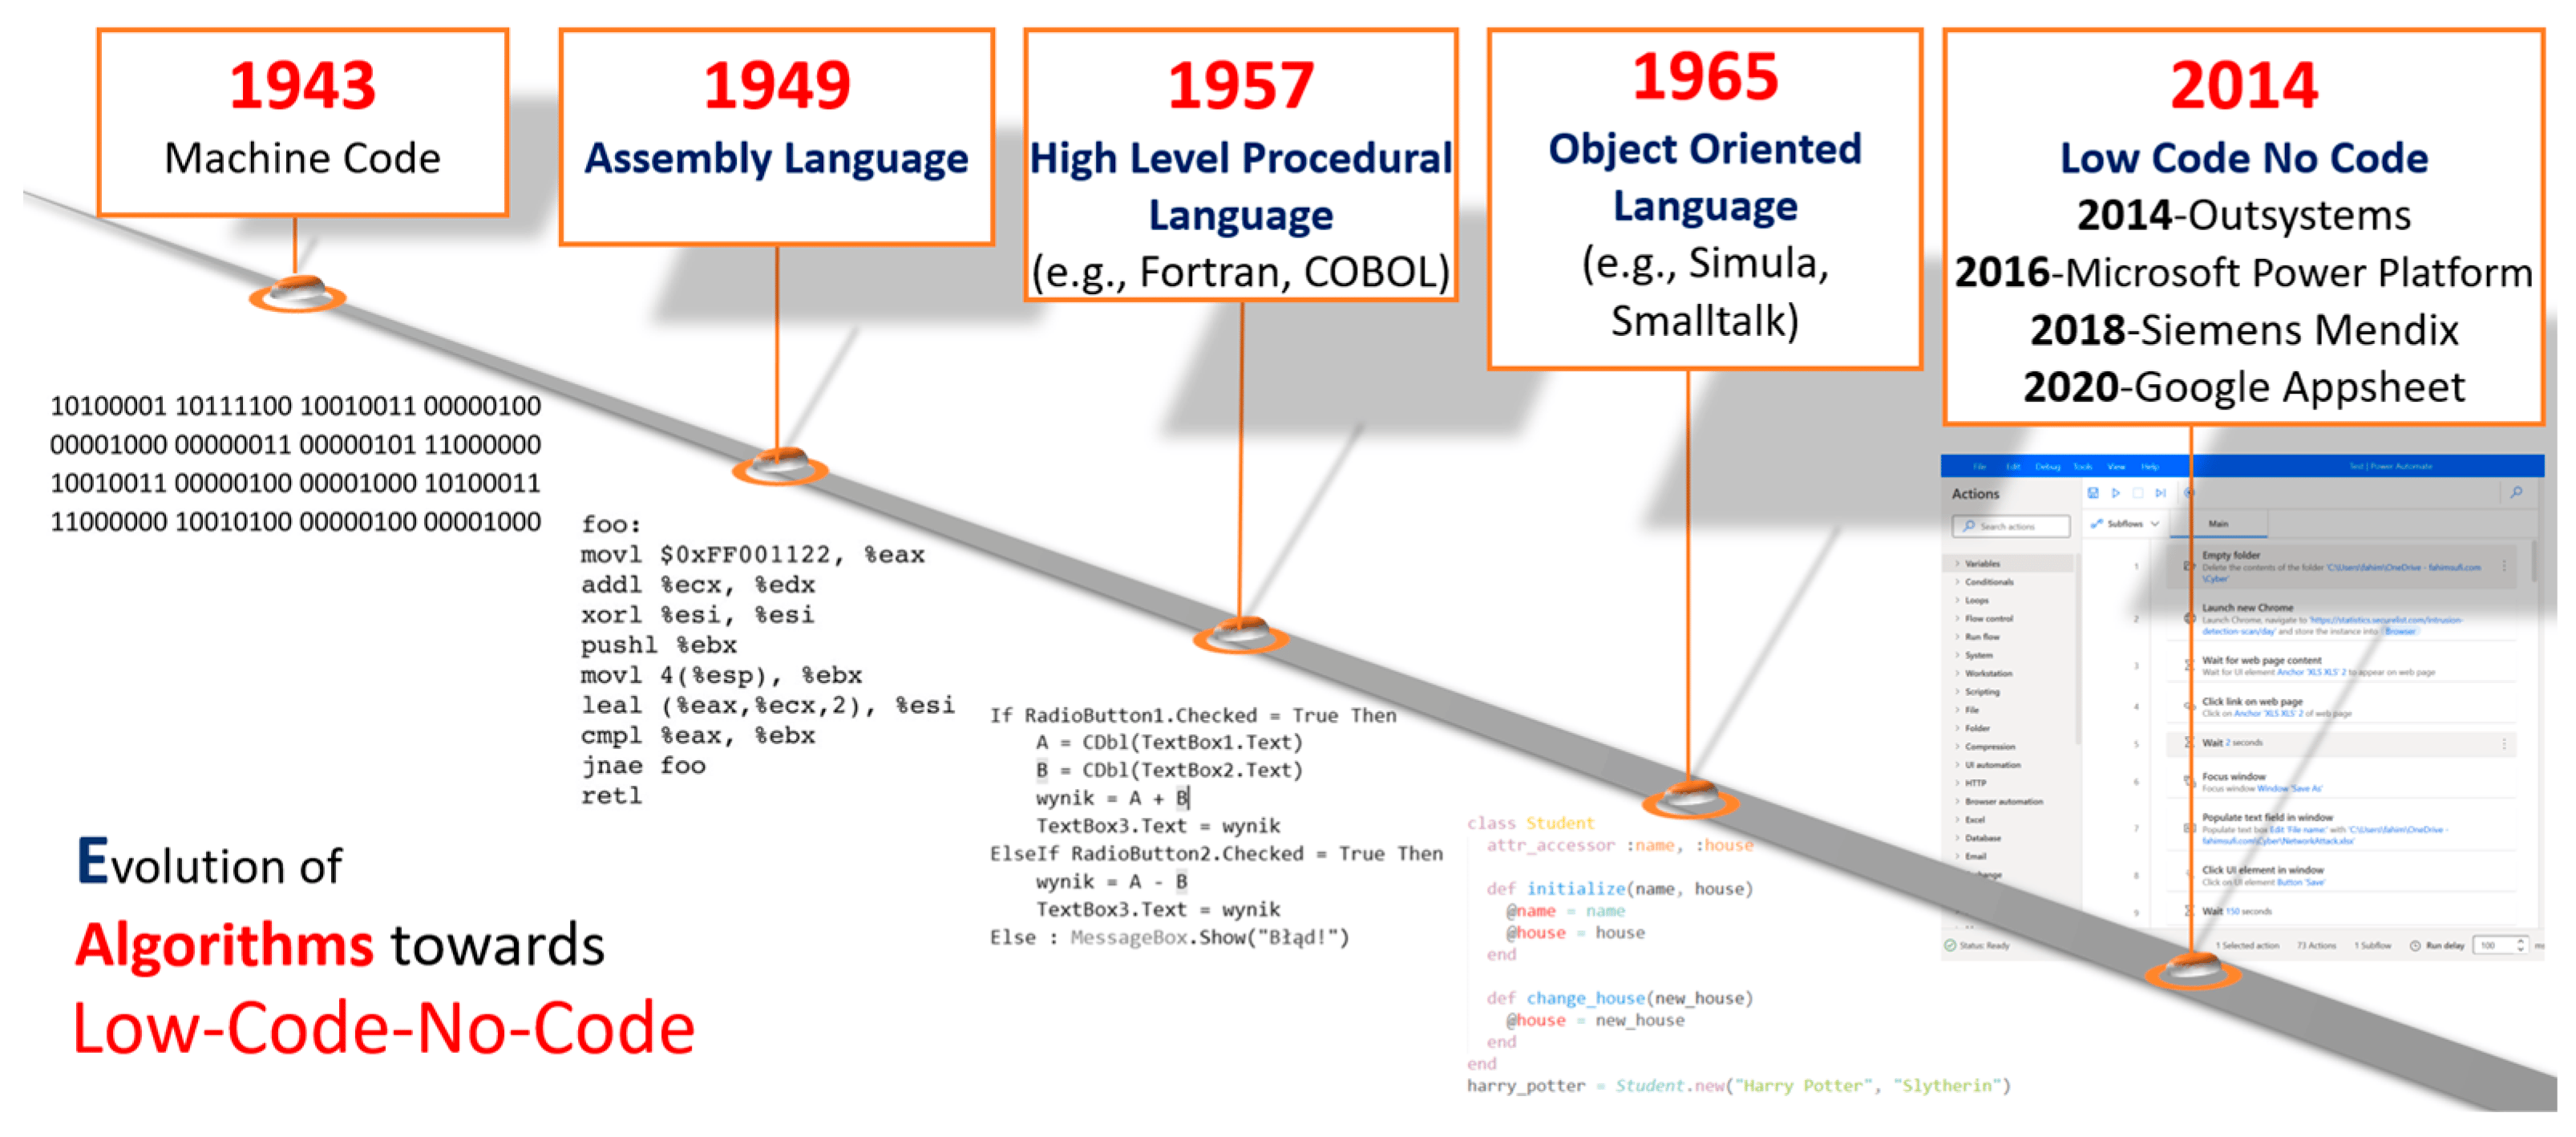
\includegraphics[width=0.8\textwidth]{Evolution_Of_Programming.jpg}
    \caption[Evolution of programming]{\label{fig:evolution} Evolutie van programmeertalen naar steeds hogere abstractieniveau \autocite{Sufi_2023}.}
\end{figure}


\subsection{\IfLanguageName{dutch}{Historische context en evolutie}{Historical Context and Evolution}}%
\gls{MDD} heeft een rijke geschiedenis die meer dan 40 jaar teruggaat \autocite{Henkel2010}. De evolutie verliep in verschillende fasen:

In de jaren '80 ontstonden de eerste geavanceerde modelleringsmethoden om de vereisten van informatiesystemen vast te leggen. Dit vormde de conceptuele basis voor \gls{MDD} \autocite{Henkel2010}.

De jaren '90 brachten propriëtaire \gls{CASE}-tools, die informatiesystemen gedeeltelijk konden genereren op basis van modellen. Deze tools hadden echter beperkingen - vaak konden ze alleen codetemplates genereren waarna programmeurs de rest handmatig moesten aanvullen \autocite{Case_1985}.

Modernere benaderingen omvatten \gls{MDA} en \gls{xUML}. \gls{MDA} werkt met verschillende modelleringsniveaus en transformaties tussen deze niveaus naar code, waarbij de gegenereerde code verder kan worden uitgewerkt \autocite{Soley2000}.\gls{xUML} daarentegen streeft naar volledige codegeneratie zonder handmatige aanvullingen.

Er bestaan grote verschillen tussen oudere \gls{CASE}-tools zoals Oracle Forms en Microsoft Access Forms en nieuwere tools gebaseerd op open standaarden zoals OptimalJ. Hoewel beide soorten tools \gls{MDD} ondersteunen door abstractieniveaus te verhogen, bieden tools zoals OptimalJ meer controle over modeltransformaties en codegeneratie, terwijl formulier-gebaseerde tools zoals Oracle Forms minder controle bieden \autocite{Henkel2010}.

Ondanks deze verschillen delen alle \gls{MDD}-benaderingen één fundamenteel doel: het verhogen van het abstractieniveau in softwareontwikkeling, waardoor ontwikkelaars complexere systemen kunnen bouwen met minder inspanning - vergelijkbaar met de evolutie van assembly-taal naar hogere programmeertalen zoals C\# en Java.


\subsection{\IfLanguageName{dutch}{Voordelen van Model-Driven Development}{Benefits of Model-Driven Development}}%
De literatuur identificeert verschillende belangrijke voordelen van het gebruik van \gls{MDD}-benaderingen \autocite{Soley2000}. Door te werken met goed gedefinieerde modellen kunnen ontwikkelaars het aantal implementatiefouten verminderen, waardoor de softwarekwaliteit verbetert. Hogere abstractieniveaus stellen ontwikkelaars in staat om zich te richten op bedrijfslogica in plaats van technische implementatiedetails, wat de productiviteit van ontwikkelaars verhoogt. Modellen geven een duidelijker inzicht in de systeemstructuur en het gedrag, waardoor het ontwikkelproces beter onder controle is.

Bovendien vermindert het automatisch genereren van code de handmatige codeerinspanning en de bijbehorende fouten, wat leidt tot lagere ontwikkel- en onderhoudskosten. Snellere ontwikkelcycli helpen organisaties efficiënter om te gaan met hun applicatieontwikkelingsbehoeften, waardoor de ontwikkelingsachterstand afneemt. De mogelijkheid om snel iteraties uit te voeren en werkende functionaliteit te demonstreren verbetert de betrokkenheid van belanghebbenden, waardoor de klanttevredenheid toeneemt.

\subsection{\IfLanguageName{dutch}{Belangrijkste functionaliteitsgebieden voor MDD-tools}{Benefits of Model-Driven Development}}%
Om een \gls{MDD}-tool effectief te laten zijn, moet het verschillende kritieke functionaliteiten ondersteunen, die kunnen worden gecategoriseerd in ondersteuning van zowel het modelleren als het ontwikkelproces.

Effectieve ondersteuning bij het modelleren vereist dat tools de juiste abstractieniveaus hanteren, waarbij irrelevante details worden verborgen terwijl essentiële concepten worden blootgelegd. 

Dit is vooral belangrijk omdat belanghebbenden modellen voor verschillende doeleinden gebruiken. Modellen moeten begrijpelijk zijn voor zowel technische als niet-technische belanghebbenden, idealiter met behulp van intuïtieve, voorspelbare notatie - veel tools maken om deze reden gebruik van \gls{UML}, omdat dit wordt beschouwd als de de-facto standaard in de industrie \autocite{Marin2015} . Modellen moeten uitvoerbaar zijn, zelfs als ze incompleet zijn, zodat incrementele ontwikkeling mogelijk is en ontwikkelaars het gedrag van het systeem kunnen voorspellen door middel van experimenten of formele analyse. 

Volwassen \gls{MDD}-tools ondersteunen de verfijning van modellen en transformaties tussen verschillende abstractieniveaus, waardoor aanpasbare model-naar-model en model-naar-code transformaties mogelijk zijn. Volgens \textcite{Marin2015} “moeten \gls{MDD}-tools de uitvoering van modellen mogelijk maken, ook al zijn ze onvolledig, maar wel geldig”, wat modelcorrectie en -validatie in een vroeg stadium vergemakkelijkt.

Ondersteuning van het ontwikkelproces omvat een reeks functies. Tools moeten duidelijke feedback geven over fouten, idealiter door direct te wijzen naar de modelcomponenten die problemen veroorzaken, vergelijkbaar met hoe compilers problematische code markeren. 
Omdat software meestal door teams wordt ontwikkeld, moeten \gls{MDD}-tools modelvergelijking, samenvoeging en versiebeheer ondersteunen. 

\textcite{Marin2015} benadrukken dat “versiebeheer van modellen absoluut noodzakelijk is om industriële samenwerkingsprojecten te beheren, waarbij verschillende leden van een ontwikkelteam aan hetzelfde model kunnen werken”.Effectieve tools moeten snel compileren en implementeren, met een bijzonder efficiënte afhandeling van incrementele wijzigingen.


\gls{MDD}-tools moeten integreren met bestaande systemen en ontwikkelomgevingen, waardoor verbindingen met ERP-systemen, legacy applicaties en andere bedrijfsinfrastructuur mogelijk worden. Een van de belangrijkste voordelen van \gls{MDD} is dat een breder scala aan mensen kan deelnemen aan de ontwikkeling, waaronder bedrijfskundigen met beperkte programmeervaardigheden. Tools moeten de definitie en het gebruik van herbruikbare componenten, patronen en best practices in projecten vergemakkelijken. 

Door deze functies op te nemen kunnen \gls{MDD}-tools beter aansluiten op de behoeften van de industrie en de succesvolle toepassing van het \gls{MDD}-paradigma in softwareontwikkelingsprojecten ondersteunen.

\subsection{\IfLanguageName{dutch}{De evolutie naar low-code platformen}{The Evolution Toward Low-Code Platforms}}%
\gls{MDD} is de laatste jaren sterk geëvolueerd, vooral met de opkomst van low-code platformen zoals Mendix. Deze platformen vertegenwoordigen een verfijning van \gls{MDD}-principes, waardoor ze toegankelijker worden voor ontwikkelaars met verschillende vaardigheidsniveaus, terwijl de kernvoordelen van modelgedreven benaderingen behouden blijven.

Zoals \textcite{Henkel2010} aantoonden in hun analyse van Mendix, proberen moderne \gls{MDD}-tools een balans te vinden tussen abstractie en controle, waardoor ontwikkelaars op bedrijfsniveau kunnen redeneren terwijl ze toch voldoende controle houden over het systeemgedrag. Deze evolutie heeft \gls{MDD}-principes toegankelijk gemaakt voor een breder publiek, waardoor softwareontwikkeling democratischer wordt dan alleen voor traditionele programmeerexperts. \textcite{Henkel2010} benadrukken dat “low-code platforms zoals Mendix met succes de kloof hebben overbrugd tussen abstractie op hoog niveau en technische implementatie, waardoor zowel zakelijke belanghebbenden als ontwikkelaars effectief kunnen samenwerken.”

Concluderend kan gesteld worden dat \gls{MDD} een significante vooruitgang betekent in software engineering methodologie, door modellen te verheffen van secundaire documentatie tot primaire ontwikkelartefacten. Door het abstractieniveau te verhogen stelt \gls{MDD} ontwikkelaars in staat om complexiteit effectiever te managen, waardoor de productiviteit kan toenemen, de kwaliteit kan verbeteren en softwareontwikkeling toegankelijker wordt voor een breder scala aan belanghebbenden.De integratie van \gls{MDD}-principes in low-code platforms heeft het bereik verder vergroot, waardoor het een krachtig hulpmiddel is geworden voor moderne softwareontwikkeling.

\section{\IfLanguageName{dutch}{Low-code platformen}{Low-code platforms}}%
In de volgende paragrafen zullen we de belangrijkste kenmerken, sterke punten en beperkingen van verschillende toonaangevende low-code ontwikkelplatformen onderzoeken en vergelijken, waaronder OutSystems, Joget DX en Mendix. Elk platform biedt unieke mogelijkheden en komt tegemoet aan verschillende organisatorische behoeften en use cases. Door hun benaderingen van visuele ontwikkeling, schaalbaarheid, inzetmogelijkheden, maatwerk en integratiemogelijkheden te onderzoeken, willen we een duidelijk inzicht geven in hoe deze platforms zich tot elkaar verhouden. Uiteindelijk zal deze vergelijking duidelijk maken waarom Mendix de meest uitgebreide en veelzijdige oplossing is, met de beste balans tussen flexibiliteit, schaalbaarheid en geavanceerde functies voor bedrijven die hun digitale transformatie willen versnellen.
\subsection{\IfLanguageName{dutch}{OutSystems}{OutSystems}}
OutSystems is een robuust low-code platform dat bekend staat om zijn uitgebreide functies en enterprise-gerichte capaciteiten. Het platform onderscheidt zich door een intuïtieve visuele ontwikkelomgeving waarmee ontwikkelaars via drag-and-drop interfaces en voorgedefinieerde componenten snel applicaties kunnen bouwen. Deze gebruiksvriendelijke interface stelt zowel ervaren ontwikkelaars als gebruikers met minder technische kennis in staat om efficiënt te werken \autocite{Sido2024}. Op het gebied van schaalbaarheid biedt OutSystems sterke prestaties voor enterprise-toepassingen, waarbij de architectuur is ontworpen om mee te groeien met toenemende gebruikersaantallen en datavolumes. Het platform ondersteunt zowel cloud-native als on-premises implementatieopties, waardoor organisaties flexibel kunnen kiezen voor de deploymentstrategie die het beste past bij hun infrastructuur en compliance-vereisten. 

\begin{figure}[H]
    \centering
    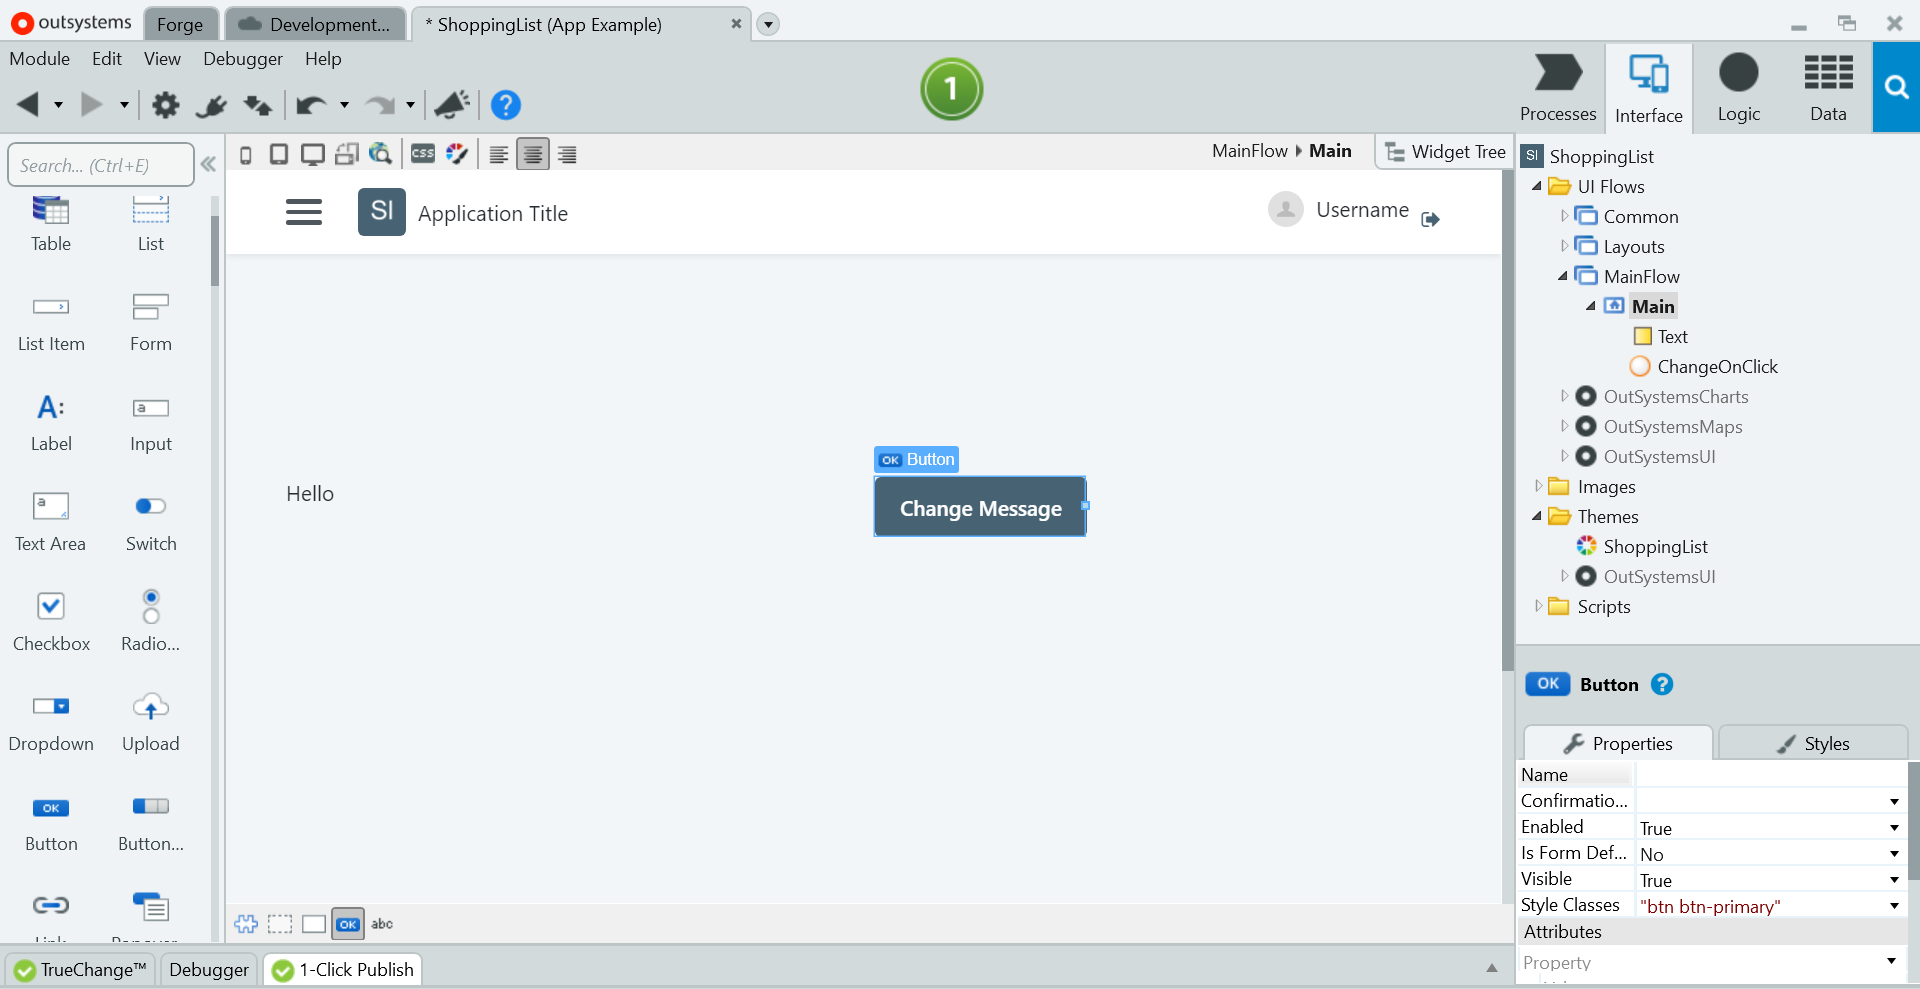
\includegraphics[width=0.8\textwidth]{OutSystems.png}
    \caption[Visuele ontwikkelomgeving Outsystems]{\label{fig:outsystems} Visuele ontwikkelomgeving van OutSystems \autocite{FigueiraPutresza2021}.}
\end{figure}


Wat betreft maatwerk biedt OutSystems uitgebreide aanpassingsmogelijkheden via eigen extensies en de integratie van custom code wanneer de standaard visuele ontwikkelingstools niet toereikend zijn. Dit stelt ontwikkelaars in staat om complexe bedrijfslogica te implementeren, hoewel dit soms ten koste kan gaan van de ontwikkelsnelheid \autocite{Sido2024}. Voor integraties beschikt het platform over diverse mogelijkheden om te koppelen met externe systemen en API's, maar er zijn beperkingen bij de integratie met sommige databases en uitdagingen bij migraties, vooral bij complexe legacy-systemen. OutSystems kan verder bogen op een levendig ecosysteem en community, samen met sterke beveiligingsfuncties en naleving van industriestandaarden. Het licentiemodel en de kostenbeperkingen kunnen echter onbetaalbaar zijn voor sommige organisaties, terwijl de kwaliteit van de documentatie en de geïsoleerde ondersteuning van de community barrières kunnen opwerpen voor ontwikkelaars die het volledige potentieel van het platform willen benutten \autocite{Sido2024}.


\subsection{\IfLanguageName{dutch}{Joget DX}{Joget DX}}
Joget DX is een open-source low-code platform dat zich onderscheidt door zijn toegankelijkheid en focus op snelle applicatieontwikkeling. Op het gebied van visuele ontwikkeling biedt het platform een intuïtieve interface die ontworpen is voor eenvoud, waardoor ook niet-technische gebruikers snel aan de slag kunnen met het bouwen van applicaties. Het is vooral sterk in de ontwikkeling van \gls{PWA}'s en legt veel nadruk op \gls{UX}, waardoor eindgebruikers kunnen profiteren van moderne, responsieve interfaces \autocite{Sido2024}. Qua schaalbaarheid kent Joget DX enkele beperkingen door het abonnementsmodel en app-beperkingen, wat uitdagingen kan opleveren voor grootschalige enterprise-toepassingen die hoge prestatie-eisen stellen.

\begin{figure}[H]
    \centering
    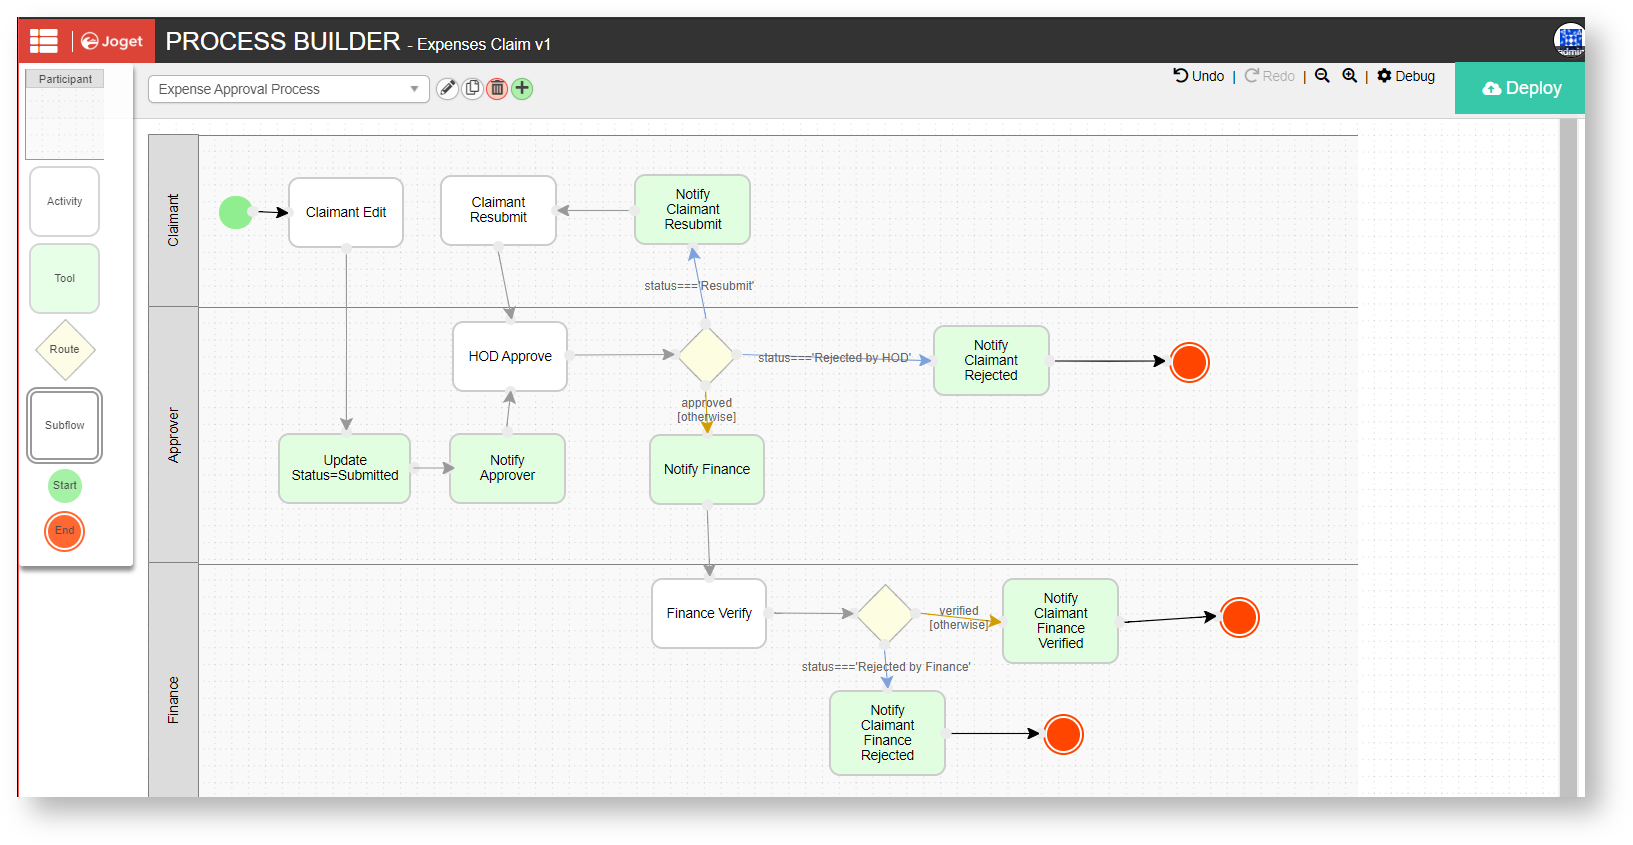
\includegraphics[width=0.8\textwidth]{JogetDx.png}
    \caption[Visuele ontwikkelomgeving Joget DX]{\label{fig:jogetDx} Visuele ontwikkelomgeving van Joget DX \autocite{Hugo2024}.}
\end{figure}

Voor inzetmogelijkheden biedt het platform goede integratie met DevOps-praktijken, waardoor het goed past binnen moderne ontwikkelworkflows en continuous delivery-processen. Het open-source karakter geeft organisaties flexibiliteit in de implementatie, hoewel de beperkte databasetoegang sommige deployment-scenario's kan bemoeilijken. Op het gebied van maatwerk beschikt Joget DX over uitbreidbaarheid via add-on builders en verbeterde workflowmogelijkheden, waardoor het een flexibele keuze is voor bedrijven die specifieke bedrijfsprocessen willen automatiseren en aanpassen aan hun behoeften \autocite{Sido2024}. De integratiemogelijkheden zijn redelijk robuust voor standaard use-cases, maar kunnen beperkingen vertonen bij complexere scenario's of legacy-systemen, wat de algehele aanpasbaarheid kan verminderen. Bovendien kunnen de leercurve en aanpassingscomplexiteit van het platform uitdagingen vormen voor gebruikers die overstappen van traditionele ontwikkelmethoden, wat extra training en gewenningstijd kan vereisen.
\subsection{\IfLanguageName{dutch}{Mendix}{Mendix}}
Mendix wordt gepositioneerd als een veelzijdig low-code platform dat een breed scala aan functies biedt voor zowel technische als niet-technische gebruikers. Het platform maakt gebruik van een modelgedreven ontwikkelaanpak, gecombineerd met microservices en containerisatie, wat bijdraagt aan de schaalbaarheid, flexibiliteit en draagbaarheid. Mendix ondersteunt zowel cloud-native als on-premise infrastructuren, wat zorgt voor flexibiliteit in de inzetmogelijkheden. Het platform biedt volledige levenscyclusbeheer, evenals functionaliteiten voor \gls{AI}, \gls{ML} en procesautomatisering, waardoor het geschikt is voor een breed scala aan zakelijke toepassingen \autocite{Sido2024}. Daarnaast biedt Mendix openheid en uitbreidbaarheid, wat integratie met externe systemen mogelijk maakt en aanpassingen voor specifieke bedrijfsbehoeften ondersteunt. Hoewel er enkele beperkingen zijn, zoals de beperkte aanpasbaarheid van thema's en het risico van vendor lock-in, bieden de functionaliteiten en het gebruiksgemak aanzienlijke voordelen \autocite{Sido2024}.

\begin{figure}[H]
    \centering
    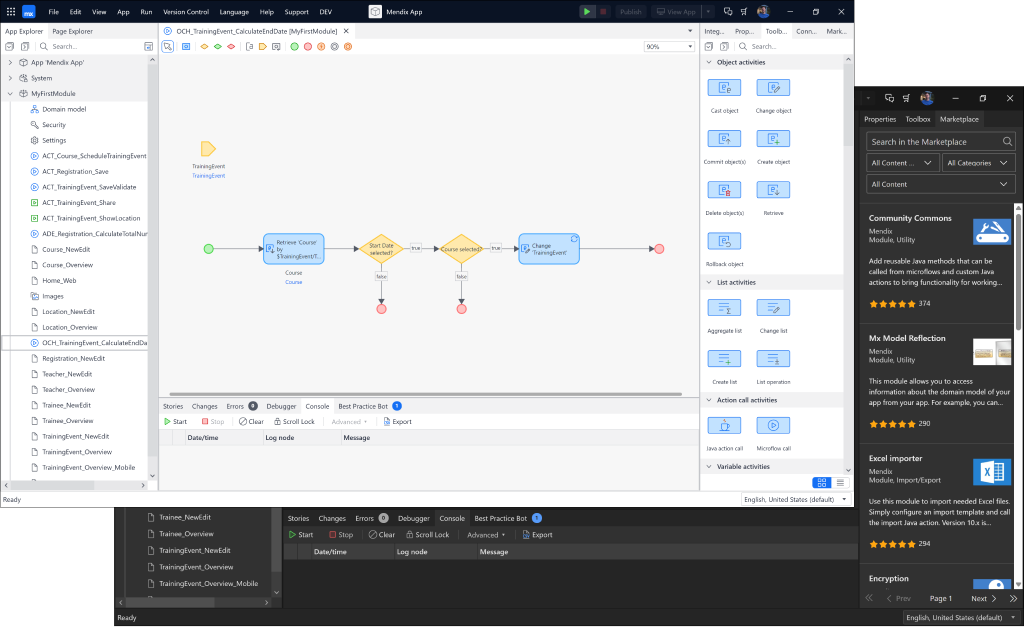
\includegraphics[width=0.8\textwidth]{Mendix.png}
    \caption[Visuele ontwikkelomgeving Mendix]{\label{fig:Mendix} Visuele ontwikkelomgeving van Mendix \autocite{Mendix2025}.}
\end{figure}


\subsection{\IfLanguageName{dutch}{Keuze voor Mendix als low-code platform}{Choosing Mendix as low-code platform}}
Hoewel OutSystems en Joget DX waardevolle functies en mogelijkheden bieden, komt Mendix naar voren als het beste platform vanwege zijn uitgebreide en flexibele benadering van low-code ontwikkeling. Zoals onderstaande vergelijkingstabel laat zien, blinkt Mendix uit op alle belangrijke criteria: visuele ontwikkeling, schaalbaarheid, inzetmogelijkheden, maatwerk en integratiemogelijkheden.
Het vermogen van Mendix om complexe bedrijfsapplicaties te ondersteunen met zijn geavanceerde visuele interface is superieur aan de concurrentie. De uitstekende schaalbaarheid voor enterprise-toepassingen overtreft de beperkingen die bij Joget DX worden ervaren. Daarnaast biedt Mendix meer veelzijdige deployment-opties dan beide concurrenten, terwijl de uitgebreide aanpassingsmogelijkheden en krachtige Microflow-editor meer flexibiliteit bieden dan de alternatieven.
Waar OutSystems worstelt met databaseintegratie en Joget DX beperkt wordt in complexere integratiescenario's, biedt Mendix uitstekende \gls{API}-integratie met uitgebreide connectors voor externe systemen. Deze combinatie van sterke punten maakt Mendix de ideale keuze voor organisaties die op efficiënte en effectieve wijze digitale transformatie willen stimuleren, ongeacht de complexiteit van hun bedrijfsprocessen of technische vereisten.

\begin{table}
    \centering
    \begin{tabular}{ |p{2cm}|p{4cm}|p{4cm}|p{4cm}|   }
        \hline
        \textbf{Criteria} & \textbf{OutSystems} & \textbf{Joget DX}  & \textbf{Mendix} \\
        \hline
        \textbf{Visuele} \newline \textbf{ontwikkel-ing}  & Intuïtieve drag-and-drop interface & Eenvoudige interface gericht op \gls{PWA}'s & Zeer gebruiksvriendelijk; geschikt voor alle niveau's \\
        \hline
        \textbf{Schaal-} \newline \textbf{baarheid} & Sterk; ontworpen voor groei & Beperkt door abonnementsmodel & Uitstekend voor enterprise; hoge belasting \\
        \hline
        \textbf{Inzet-} \newline \textbf{mogelijk-} \newline \textbf{heden}  & Cloud en on-premises opties & DevOps-integratie; beperkte database-opties & Veelzijdig (cloud/on-premises/hybrid); CI/CD-integratie \\
        \hline
        \textbf{Maatwerk}  & Extensies en custom code mogelijk & Add-on builders; goede workflows & Uitgebreid; Java-extensies; krachtige Microflow \\
        \hline
        \textbf{Integratie} \newline \textbf{mogelijk-} \newline \textbf{heden} & Diverse opties; enkele database-beperkingen & Adequaat voor standaard gebruik; beperkingen bij complexiteit  & Uitstekende \gls{API}'s; veel connectors; legacy-ondersteuning\\
        \hline
    \end{tabular}
    \caption[\centering Low-Code Platforms Comparison]{\label{tab:Vergelijking Low-code platformen}Vergelijking Low-code platformen.}
\end{table}

\section{Mendix en high-code}
\subsection{Verschillende benaderingen}
Low-code en high-code representeren twee verschillende benaderingen van softwareontwikkeling, elk met unieke voordelen en uitdagingen. Low-code platforms, zoals Mendix, bieden een visuele ontwikkelomgeving waarin applicaties grotendeels zonder handmatig programmeren kunnen worden gebouwd \autocite{Krouwel_2022}. Dit versnelt de ontwikkeltijd en maakt softwareontwikkeling toegankelijker voor niet-technische gebruikers. Daarentegen biedt high-code, waarbij programmeertalen zoals Java of .NET worden gebruikt, maximale flexibiliteit en controle, wat essentieel is voor complexe of sterk aangepaste oplossingen \autocite{Krouwel_2022}. Hoewel low-code efficiënter is en snellere iteraties mogelijk maakt, kan het beperkingen hebben in maatwerk en prestaties vergeleken met high-code. De keuze tussen beide hangt af van de behoeften van de organisatie: low-code is ideaal voor snelle, aanpasbare applicaties, terwijl high-code de voorkeur geniet voor diepgaande technische en schaalbare oplossingen.

\subsection{Enterprise Flexibiliteit door Model-Based Engineering}
\textcite{Krouwel_2022} benadrukt dat enterprise agility een cruciale succesfactor is in een steeds dynamischere markt, waarin bedrijven te maken hebben met hyperconcurrentie, veranderende regelgeving en technologische innovaties. Traditionele informatiesystemen vormen vaak een beperkende factor voor deze flexibiliteit, omdat ze hardcoded bedrijfsregels en structuren bevatten die moeilijk aanpasbaar zijn. Door \gls{MBE} te gebruiken, kunnen organisaties hun informatiesystemen ontwikkelen op basis van ontologische modellen, zoals die binnen de \gls{DEMO}-methodologie worden gehanteerd. Deze modellen beschrijven de essentiële processen en interacties binnen een onderneming, los van specifieke implementaties. Dit maakt het mogelijk om snel en systematisch wijzigingen door te voeren, zonder dat ontwikkelaars handmatig code hoeven aan te passen. Het resultaat is een grotere wendbaarheid van zowel de organisatie als haar IT-systemen, waardoor bedrijven sneller kunnen inspelen op veranderingen zonder dat technologie een beperkende factor vormt

\subsection{Low-Code als Brug tussen Business en IT}
Een belangrijke conclusie uit \textcite{Krouwel_2022} is dat low-code technologie niet alleen zorgt voor een snellere ontwikkeling van software, maar ook de samenwerking tussen business en IT aanzienlijk verbetert. Traditionele softwareontwikkeling vereist vaak uitgebreide specificaties en langdurige communicatie tussen ontwikkelaars en business stakeholders, wat leidt tot vertragingen en misinterpretaties. Low-code platforms, zoals Mendix, bieden een visuele ontwikkelomgeving waarin bedrijfsgebruikers direct kunnen meedenken en bijdragen aan het ontwerp van applicaties \autocite{Mendix}. Dit verlaagt de drempel om wijzigingen door te voeren en zorgt ervoor dat IT-systemen beter aansluiten op de behoeften van de organisatie. Doordat bedrijfsprocessen en bijbehorende applicaties sneller en effectiever kunnen worden aangepast, wordt de time-to-market verkort en kunnen organisaties flexibeler inspelen op nieuwe kansen en uitdagingen

\subsection{Kunnen beiden elkaar aanvullen?}
Volgens \textcite{Krouwel_2022} kunnen low-code en high-code elkaar versterken door de flexibiliteit van \gls{MBE} te combineren met de aanpasbaarheid van traditionele codering. Low-code platforms zoals Mendix maken gebruik van abstracties en modelgestuurde technieken, waardoor applicaties sneller kunnen worden ontwikkeld zonder dat complexe code nodig is. Tegelijkertijd biedt high-code de mogelijkheid om de gegenereerde applicaties verder te verfijnen, bijvoorbeeld door aangepaste logica, integraties of prestatie-optimalisaties toe te voegen. In het onderzoek wordt benadrukt dat low-code vooral geschikt is om snel te reageren op veranderingen in bedrijfsprocessen, terwijl high-code nodig blijft voor diepgaande aanpassingen en geavanceerde automatiseringen. Door beide methoden te combineren, ontstaat een hybride aanpak waarbij organisaties profiteren van de snelheid en wendbaarheid van low-code zonder in te boeten op de kracht en maatwerkopties van high-code.

\section{Keuze tussen high-code en low-code?}
Bij het kiezen tussen high-code en low-code ontwikkelmethoden is het essentieel om vooraf duidelijk te bepalen welke functionaliteiten en mate van maatwerk je voor je applicatie nodig hebt \autocite{Ballejos2024}. High-code ontwikkeling biedt maximale flexibiliteit en is geschikt voor complexe, op maat gemaakte oplossingen, maar vereist aanzienlijke tijd en technische expertise. Low-code platforms versnellen het ontwikkelproces door gebruik te maken van visuele tools en vooraf gebouwde componenten, wat ideaal is voor applicaties die snel moeten worden ontwikkeld met een zekere mate van aanpasbaarheid \autocite{Ballejos2024}.  Door vooraf je specifieke eisen en doelen te definiëren, kun je de ontwikkelmethode kiezen die het beste aansluit bij de behoeften van je project en organisatie.



    %%=============================================================================
%% Methodologie
%%=============================================================================

\chapter{\IfLanguageName{dutch}{Methodologie}{Methodology}}%
\label{ch:methodologie}

%% TODO: In dit hoofstuk geef je een korte toelichting over hoe je te werk bent
%% gegaan. Verdeel je onderzoek in grote fasen, en licht in elke fase toe wat
%% de doelstelling was, welke deliverables daar uit gekomen zijn, en welke
%% onderzoeksmethoden je daarbij toegepast hebt. Verantwoord waarom je
%% op deze manier te werk gegaan bent.
%% 
%% Voorbeelden van zulke fasen zijn: literatuurstudie, opstellen van een
%% requirements-analyse, opstellen long-list (bij vergelijkende studie),
%% selectie van geschikte tools (bij vergelijkende studie, "short-list"),
%% opzetten testopstelling/PoC, uitvoeren testen en verzamelen
%% van resultaten, analyse van resultaten, ...
%%
%% !!!!! LET OP !!!!!
%%
%% Het is uitdrukkelijk NIET de bedoeling dat je het grootste deel van de corpus
%% van je bachelorproef in dit hoofstuk verwerkt! Dit hoofdstuk is eerder een
%% kort overzicht van je plan van aanpak.
%%
%% Maak voor elke fase (behalve het literatuuronderzoek) een NIEUW HOOFDSTUK aan
%% en geef het een gepaste titel.

Dit onderzoek is opgedeeld in twee fasen: eerst het in kaart brengen van het probleemdomein (het ontbreken van een beslissingskader), gevolgd door onderzoek naar het oplossingsdomein (de ontwikkeling van het kader).
\section{Fase 1: Analyse van het probleemdomein}
Om een grondig inzicht te krijgen in het probleemdomein worden de volgende onderzoeksmethoden gebruikt:
\subsection{Analyse van historische projectdata}
Om deelvragen 1 en 2 te beantwoorden ("Wat zijn de gevolgen van het ontbreken van een beslissingskader?" \; \hbox{en} \, "Welke problemen ontstaan er in projecten?"), wordt een gestructureerde analyse uitgevoerd van afgesloten projecten. Bij deze analyse worden initiële projectschattingen vergeleken met werkelijke uitkomsten om de impact op kosten en doorlooptijd nauwkeurig te kwantificeren. Daarnaast wordt de projectdocumentatie systematisch doorgenomen met als doel het identificeren van specifieke momenten waarop keuzes tussen low-code en high-code ontwikkelmethoden tot problemen hebben geleid. Het onderzoek inventariseert ook situaties waarin projectteams gedwongen waren om tijdens het project over te schakelen naar alternatieve ontwikkelmethoden vanwege onvoorziene beperkingen. Ten slotte wordt de financiële en tijdsimpact van deze late aanpassingen grondig geëvalueerd om de werkelijke kosten van suboptimale initiële technologiekeuzes inzichtelijk te maken.
\subsection{Interviews met experts}
Voor het beantwoorden van deelvragen 3 en 4 ("Wat zijn de huidige criteria?" \; \hbox{en} \, "Welke knelpunten ervaren projectmanagers?") worden diepte-interviews gehouden met verschillende belanghebbenden binnen het ontwikkelproces. Projectmanagers worden geïnterviewd over hun huidige besluitvormingsproces bij technologiekeuzes, waarbij specifiek wordt gefocust op de impliciete en expliciete criteria die zij hanteren. Daarnaast delen architecten hun ervaringen met technologie-keuzes, inclusief de technische overwegingen die doorslaggevend zijn bij het maken van platformkeuzes. Pre-sales consultants worden bevraagd over hun methodiek bij het inschatten van projectgeschiktheid voor verschillende ontwikkelplatformen in de offertefase. Tot slot worden ontwikkelaars geïnterviewd over de praktische uitdagingen die zij ervaren wanneer technologiekeuzes zijn gemaakt en zij deze moeten implementeren, met bijzondere aandacht voor de discrepantie tussen verwachtingen en werkelijkheid.
\subsection{Documentatieonderzoek}
Om deelvraag 3 verder te onderbouwen wordt bestaande interne documentatie geanalyseerd. Dit omvat een grondige bestudering van de huidige richtlijnen en procedures voor projectaanpak, waarin impliciet of expliciet keuzes worden gemaakt over ontwikkelmethoden. Ook worden pre-sales documentatie en offertes onder de loep genomen om inzicht te krijgen in de initiële afwegingen en beloftes die worden gedaan voordat een project daadwerkelijk start. Project kick-off documenten worden onderzocht om de uitgangspunten en verwachtingen aan het begin van projecten te identificeren, met specifieke aandacht voor de technologiekeuzes die in deze vroege fase worden vastgelegd. Tenslotte worden architectuurbeslissingen en design documents geanalyseerd om te begrijpen hoe technische overwegingen worden gedocumenteerd en gecommuniceerd binnen projectteams, en hoe deze documenten bijdragen aan het besluitvormingsproces rondom low-code versus high-code ontwikkeling.

\section{Fase 2: Onderzoek naar het oplossingsdomein}
Na het volledig in kaart brengen van het probleem, richt het onderzoek zich op het ontwikkelen van een oplossing middels:
\subsection{Literatuuroverzicht}
Een diepgaande analyse van bestaande documentatie over Mendix en andere low-code platforms vormt een essentieel onderdeel voor het beantwoorden van deelvraag 5 en 7. Deze analyse omvat diverse bronnen, waaronder officiële Mendix productgidsen die gedetailleerde technische specificaties en functionaliteiten beschrijven, casestudies van derden en rapporten uit de industrie die praktijkvoorbeelden en onafhankelijke evaluaties bieden, online forums en ontwikkelaarsgemeenschappen waar praktijkervaringen en knelpunten worden gedeeld, en academische publicaties over low-code ontwikkeling die theoretische onderbouwing en wetenschappelijke inzichten verschaffen over de bredere context van deze technologie.
\subsection{Praktisch onderzoek}
Voor de beantwoording van deelvraag 6 worden praktische tests uitgevoerd om de grenzen van het Mendix-platform te onderzoeken. Dit onderzoek richt zich op verschillende aspecten, waaronder schaalbaarheid en prestaties, waarbij de reactietijd, belastingstestresultaten en het vermogen om te schalen bij toenemende gebruikersaantallen worden geëvalueerd. Daarnaast worden de integratiemogelijkheden getest om de compatibiliteit met externe systemen, API’s en databases te beoordelen. De aanpasbaarheid en uitbreidbaarheid van het platform worden geanalyseerd door te onderzoeken in hoeverre maatwerkfunctionaliteiten en uitbreidingen kunnen worden geïmplementeerd. Ook de ontwikkelingssnelheid wordt onder de loep genomen, waarbij wordt gekeken naar de efficiëntie van de ontwikkelomgeving en de snelheid waarmee applicaties kunnen worden gebouwd en aangepast. Tot slot wordt de beveiliging en compliance beoordeeld om vast te stellen in hoeverre het platform voldoet aan relevante regelgeving en beveiligingsstandaarden. Deze tests bieden een diepgaand inzicht in de sterke en zwakke punten van Mendix en helpen bij het bepalen van de geschiktheid van het platform voor specifieke toepassingen.

\subsection{Reflectie op eigen ervaringen}
In dit onderzoek wordt een gestructureerde reflectie uitgevoerd op de transitie van high-code naar low-code ontwikkeling binnen een lopend Mendix-project. Hierbij worden persoonlijke ervaringen gedocumenteerd, waarbij zowel de uitdagingen als successen in de praktijk worden belicht. Er wordt een vergelijkende analyse gemaakt van de ontwikkelingsefficiëntie tussen traditionele high-code methoden en de Mendix-aanpak, met aandacht voor de verschillen in snelheid, flexibiliteit en onderhoudbaarheid. Daarnaast worden specifieke situaties geïdentificeerd waarin high-code kennis een toegevoegde waarde biedt binnen een Mendix-omgeving, bijvoorbeeld bij complexe logica of integraties met externe systemen. Tot slot wordt de leercurve geëvalueerd en worden de benodigde aanpassingen in denkwijze besproken die gepaard gaan met de overstap naar een low-code platform. Deze reflectie biedt waardevolle inzichten in de impact van low-code ontwikkeling op bestaande programmeerervaringen en werkwijzen.

\subsection{Evaluatie van Mendix-uitbreidingen}
In dit onderzoek wordt de effectiviteit van verschillende uitbreidingsstrategieën voor Mendix geanalyseerd. Een belangrijk aspect daarbij is de vergelijking tussen standaard Marketplace-modules en custom ontwikkeling, waarbij wordt gekeken naar factoren zoals flexibiliteit, implementatietijd en onderhoudsgemak. Daarnaast wordt de impact van Java-uitbreidingen onderzocht, met specifieke aandacht voor de invloed op onderhoudbaarheid en toekomstbestendigheid van het platform. Ook wordt een analyse uitgevoerd van de kosten-batenverhouding van verschillende uitbreidingsmethoden, waarbij zowel ontwikkel- als beheerkosten worden meegenomen. Tot slot worden de integratie-uitdagingen beoordeeld die zich voordoen bij het combineren van Mendix met externe systemen en services, om zo inzicht te krijgen in de haalbaarheid en complexiteit van verschillende uitbreidingsopties. Deze analyse draagt bij aan een beter begrip van de meest effectieve strategieën voor het uitbreiden van Mendix-toepassingen binnen verschillende bedrijfscontexten.

\subsection{Ontwikkeling beslissingskader}
Voor het beantwoorden van deelvraag 8, die zich richt op het destilleren van best practices en richtlijnen voor de keuze tussen Mendix en traditionele ontwikkeling, wordt een gestructureerd beslissingskader ontwikkeld. Dit kader ondersteunt projectmanagers en architecten bij het maken van weloverwogen keuzes over de inzet van Mendix in vergelijking met conventionele ontwikkelmethoden. Het biedt beslissingspunten voor de initiële keuze tussen Mendix en traditionele ontwikkeling en stelt criteria vast om te bepalen welke projectonderdelen beter geschikt zijn voor high-code ontwikkeling. Daarnaast worden richtlijnen geformuleerd voor het effectief combineren van low-code en high-code in hybride projecten, zodat beide benaderingen optimaal kunnen worden ingezet. Verder bevat het kader aanbevelingen voor de vroege identificatie van potentiële beperkingen en risico’s, waardoor projectrisico’s proactief kunnen worden gemitigeerd. Tot slot worden strategieën ontwikkeld om op basis van eerdere ervaringen en literatuur weloverwogen keuzes te maken bij toekomstige projecten. Dit beslissingskader draagt bij aan een systematische en onderbouwde aanpak voor het selecteren van de meest geschikte ontwikkelmethode binnen uiteenlopende projectcontexten.



    %%=============================================================================
%% Methodologie
%%=============================================================================

\chapter{\IfLanguageName{dutch}{In kaart brengen van het probleemdomein}{Results}}%
\label{ch:resultaten}

%% TODO: In dit hoofstuk geef je een korte toelichting over hoe je te werk bent
%% gegaan. Verdeel je onderzoek in grote fasen, en licht in elke fase toe wat
%% de doelstelling was, welke deliverables daar uit gekomen zijn, en welke
%% onderzoeksmethoden je daarbij toegepast hebt. Verantwoord waarom je
%% op deze manier te werk gegaan bent.
%% 
%% Voorbeelden van zulke fasen zijn: literatuurstudie, opstellen van een
%% requirements-analyse, opstellen long-list (bij vergelijkende studie),
%% selectie van geschikte tools (bij vergelijkende studie, "short-list"),
%% opzetten testopstelling/PoC, uitvoeren testen en verzamelen
%% van resultaten, analyse van resultaten, ...
%%
%% !!!!! LET OP !!!!!
%%
%% Het is uitdrukkelijk NIET de bedoeling dat je het grootste deel van de corpus
%% van je bachelorproef in dit hoofstuk verwerkt! Dit hoofdstuk is eerder een
%% kort overzicht van je plan van aanpak.
%%
%% Maak voor elke fase (behalve het literatuuronderzoek) een NIEUW HOOFDSTUK aan
%% en geef het een gepaste titel.

\section{Analyse van historische projectdata}
In de samenwerking tussen Apvine en \gls{FOD MOB}, een klant met een intern Java-developmentteam, komt de keuze tussen high-code en low-code regelmatig terug als een belangrijk discussiepunt. Het ontbreken van een duidelijk en gestructureerd beslissingskader bemoeilijkt het maken van weloverwogen technologisch onderbouwde keuzes, wat vaak leidt tot suboptimale beslissingen. Dit maakt \gls{FOD MOB} tot een uitstekend casevoorbeeld om de gevolgen van besluiteloosheid en het ontbreken van heldere richtlijnen in het technologiekeuzeproces te analyseren. In dit onderzoek worden initiële projectschattingen vergeleken met de werkelijke uitkomsten, met als doel de impact op kosten en doorlooptijd nauwkeurig te kwantificeren. Daarnaast wordt de projectdocumentatie systematisch doorgenomen om concrete momenten te identificeren waarop de keuze tussen low-code en high-code tot frictie heeft geleid. Het onderzoek inventariseert ook in welke gevallen projectteams, bijvoorbeeld binnen \gls{FOD MOB}, gedwongen waren om tijdens het project over te schakelen naar alternatieve ontwikkelmethoden, als gevolg van onvoorziene beperkingen van het gekozen platform of ontwikkelparadigma. De financiële en tijdsimpact van deze late aanpassingen wordt vervolgens grondig geëvalueerd, om de werkelijke kosten van een gebrekkig technologisch beslissingskader inzichtelijk te maken.
\\
\\
Het ontbreken van een duidelijk beslissingskader heeft aanzienlijke gevolgen voor de technologische keuzes binnen de samenwerking tussen Apvine en \gls{FOD MOB}. In plaats van op objectieve criteria en een gestructureerd evaluatieproces te vertrouwen, worden de keuzes voor high-code versus low-code vaak beïnvloed door informele voorkeuren en machtsverhoudingen binnen het team. Dit gebrek aan een formele en transparante methodologie leidt tot verschillende problemen die de effectiviteit van het project kunnen ondermijnen:
\paragraph{Onzekerheid in de technologiekeuze}
Zonder een duidelijk beslissingskader is het voor betrokkenen moeilijk om met zekerheid te bepalen welke technologie het beste past bij de specifieke projectvereisten. Dit leidt vaak tot keuzes die niet goed afgestemd zijn op de werkelijke behoeften van het project, wat in de praktijk kan resulteren in inefficiëntie en suboptimale resultaten.
\paragraph{Frictie binnen het projectteam}
Wanneer er geen duidelijke richtlijnen zijn voor het maken van technologische keuzes, ontstaat er vaak frictie binnen het projectteam. Teamleden hebben mogelijk verschillende opvattingen over de voor- en nadelen van low-code versus high-code, wat leidt tot onduidelijkheid en conflicten. Dit vergroot de kans op vertragingen, aangezien beslissingen niet snel genomen kunnen worden door gebrek aan consensus.
\paragraph{Vertraagde besluitvorming}
Het proces van het maken van een keuze wordt uitgesteld of herhaald, omdat er geen objectief beslissingskader is om de discussie te structureren. Deze vertragingen kunnen het project belemmeren, vooral in de vroege fasen waarin cruciale technologische keuzes gemaakt moeten worden. Dit vertraagt de voortgang van het project en kan leiden tot hogere kosten en een langere doorlooptijd.
\paragraph{Noodzaak tot herziening van keuzes}
Wanneer er geen formele afstemming en evaluatie plaatsvindt, worden technologische keuzes vaak pas later in het project beoordeeld. Dit kan betekenen dat gekozen technologieën niet voldoen aan de functionele eisen, schaalbaarheid of onderhoudsvereisten. Het projectteam moet dan dure en tijdrovende herzieningen doorvoeren, zoals het aanpassen van architectuur of het implementeren van alternatieve technologieën, wat het project verder vertraagt en de kosten verhoogt.
\\
\\
Kortom, het ontbreken van een helder beslissingskader maakt het lastig om weloverwogen keuzes te maken, verhoogt de kans op interne conflicten en vertragingen, en leidt uiteindelijk tot een verhoogd risico op het maken van suboptimale technologische keuzes die de voortgang en het succes van het project belemmeren.

\section{Interviews met experts}
TODO
\\
\\
Binnen deze interviews worden projectmanagers van Apvine bevraagd over hun huidige besluitvormingsproces bij het selecteren van technologieën. Apvine is een bedrijf dat zich hoofdzakelijk richt op low-code ontwikkeling, waardoor de keuze voor een low-code platform vaak als uitgangspunt wordt genomen in plaats van als open vraag. Deze commerciële en strategische voorkeur kan een significante invloed uitoefenen op de manier waarop projectmanagers technologische keuzes benaderen, en op hoe zij hun beslissingen motiveren tegenover klanten zoals \gls{FOD MOB}.

Er wordt in de interviews expliciet gefocust op zowel de expliciete als impliciete criteria die zij hanteren bij het maken van een keuze tussen low-code en high-code trajecten. In de praktijk blijkt dat deze afweging zelden volledig neutraal wordt gemaakt: projectmanagers proberen vaak de voordelen van low-code te benadrukken en mogelijke beperkingen ervan te relativeren om het platform te positioneren als een geschikte oplossing. Hierbij is het interessant om te onderzoeken in welke mate risico-inschatting, technische haalbaarheid en klantverwachtingen werkelijk een rol spelen in hun besluitvorming, of eerder achteraf worden gebruikt om een reeds gemaakte keuze te onderbouwen.

In de interviews wordt nagegaan hoe projectmanagers omgaan met de inherente voorkeur voor low-code binnen Apvine, en hoe dit hun technologische keuzes beïnvloedt. Aangezien low-code ontwikkeling een fundamenteel onderdeel vormt van de bedrijfsstrategie, is het interessant om te verkennen in hoeverre projectmanagers ruimte ervaren om alternatieven te overwegen wanneer de klantnoden of projectvereisten daar mogelijk om vragen. Daarnaast wordt onderzocht hoe zij omgaan met situaties waarin low-code minder geschikt blijkt, en of er intern ruimte bestaat om de beperkingen van het platform te erkennen of dat men voornamelijk inzet op het verdedigen van de gekozen oplossing.

Vragen voor deze interviews: 
\begin{itemize} 
    \item Welke stappen doorloopt u typisch bij het maken van een technologiekeuze voor een nieuw project? 
    \item Welke criteria weegt u het zwaarst bij de keuze tussen low-code en high-code? 
    \item In hoeverre is uw beslissing gebaseerd op objectieve data versus ervaring of intuïtie? 
    \item Worden deze criteria vastgelegd of zijn ze vooral impliciet aanwezig? 
    \item Hoe gaat u om met klanten die een voorkeur hebben voor high-code of sceptisch staan tegenover low-code? 
    \item Kunt u een voorbeeld geven van een project waarbij low-code achteraf gezien niet de beste keuze bleek? 
\end{itemize}



Daarnaast delen solution- en softwarearchitecten hun ervaringen met technologiekeuzes. Zij geven inzicht in de doorslaggevende technische overwegingen, zoals schaalbaarheid, integratiemogelijkheden en lange termijn onderhoud, die zij meenemen bij het adviseren over platformkeuzes binnen de context van \gls{FOD MOB}-projecten.

Ook pre-sales consultants van Apvine worden geïnterviewd, met de focus op hun aanpak tijdens de offerte- en analysefase. Zij lichten toe hoe zij per project inschatten welk ontwikkelplatform het meest geschikt is, welke informatie ze hiervoor nodig hebben van de klant (zoals \gls{FOD MOB}), en welke aannames hierin een rol spelen.

Tot slot worden ontwikkelaars van Apvine zelf geïnterviewd over de praktische implicaties van gemaakte technologiekeuzes. Hierbij komt vooral de kloof tussen verwachtingen en realiteit aan bod, zoals technische beperkingen die pas tijdens de implementatie duidelijk worden, of de noodzaak om onderdelen alsnog in high-code te herschrijven vanwege beperkingen van het gekozen low-code platform.


\section{Documentatieonderzoek}
TODO
\\
\\
Om deelvraag 3 verder te onderbouwen wordt bestaande interne documentatie geanalyseerd. Dit omvat een grondige bestudering van de huidige richtlijnen en procedures voor projectaanpak, waarin impliciet of expliciet keuzes worden gemaakt over ontwikkelmethoden. Ook worden pre-sales documentatie en offertes onder de loep genomen om inzicht te krijgen in de initiële afwegingen en beloftes die worden gedaan voordat een project daadwerkelijk start. Project kick-off documenten worden onderzocht om de uitgangspunten en verwachtingen aan het begin van projecten te identificeren, met specifieke aandacht voor de technologiekeuzes die in deze vroege fase worden vastgelegd. Tenslotte worden architectuurbeslissingen en design documents geanalyseerd om te begrijpen hoe technische overwegingen worden gedocumenteerd en gecommuniceerd binnen projectteams, en hoe deze documenten bijdragen aan het besluitvormingsproces rondom low-code versus high-code ontwikkeling.
\section{Analyse van kritieke use cases}
TODO
\\
\\
Om inzicht te krijgen in de beperkingen van Mendix in praktijksituaties worden specifieke use cases onderzocht waar Mendix in zijn standaardvorm tekortschoot. Dit onderzoek begint met de identificatie van projecten waarin aanvullende modules of custom ontwikkeling noodzakelijk waren om aan de projectvereisten te voldoen. Vervolgens worden de onderliggende redenen geanalyseerd waarom de standaard Mendix-functionaliteit in deze gevallen niet toereikend bleek, waarbij zowel technische als functionele beperkingen worden gedocumenteerd. De impact van deze tekortkomingen op projectdoorlooptijd en budget wordt nauwkeurig beoordeeld om de werkelijke kosten van deze beperkingen te kwantificeren. Daarnaast wordt de effectiviteit van de geïmplementeerde aanvullende oplossingen geëvalueerd om te bepalen in hoeverre deze de oorspronkelijke beperkingen succesvol hebben geadresseerd. Tot slot worden de gevonden scenario's gecategoriseerd om patronen te identificeren in situaties waarin Mendix-uitbreidingen typisch nodig zijn, wat waardevolle input vormt voor het te ontwikkelen beslissingskader.







    %%=============================================================================
%% Methodologie
%%=============================================================================

\chapter{\IfLanguageName{dutch}{Hoe kan het beter?}{Results}}%
\label{ch:beter}



\section{Literatuuroverzicht}

In aanvulling op de eerder besproken stand van zaken biedt dit literatuuroverzicht een verdiepend inzicht in het gebruik van Mendix als low-code platform op basis van bestaande literatuur, praktijkcases en academisch onderzoek. Het platform, dat bekend staat om zijn visuele ontwikkelomgeving en ondersteuning voor zowel professionele als niet-technische gebruikers, wordt steeds vaker ingezet voor snelle en iteratieve applicatieontwikkeling \autocite{Alamin2021}. Daarnaast zijn er diverse praktijkvoorbeelden en academische analyses die de voordelen en beperkingen van low-code ontwikkeling, en Mendix in het bijzonder, verder belichten \autocite{Gadia2025}.
\subsection{Praktijkvoorbeelden en Casestudies}
Diverse organisaties hebben Mendix succesvol ingezet voor uiteenlopende toepassingen:
\begin{itemize}
    \item \textbf{Gemeente Rotterdam}
    \\
    Door het gebruik van Mendix heeft de gemeente meer dan 100 low-code applicaties ontwikkeld, waaronder een COVID-responsportaal en een parkeervergunning-app. Deze applicaties ondersteunen meer dan 100.000 gebruikers en zijn gemiddeld binnen 8-12 weken ontwikkeld \autocite{Mendix2025a}.
    \item \textbf{PostNL}
    \\
    Het nationale postbedrijf van Nederland heeft zijn ordermanagementsysteem herbouwd met Mendix, gebruikmakend van een microservices-architectuur. Hierdoor kunnen ze meer dan 1 miljoen pakketten per dag verwerken en hebben ze een achterstand van twee jaar in zes maanden weggewerkt \autocite{Zaman2024}.
    \item \textbf{AZL}
    \\
    Deze pensioenfondsbeheerder heeft met Mendix een klantportaal ontwikkeld dat het pensioenkeuzeproces voor deelnemers vereenvoudigt. Door de overstap naar een agile werkwijze in combinatie met low-code ontwikkeling, konden ze sneller inspelen op klantbehoeften en de gebruikerservaring verbeteren \autocite{MendixAZL}.
\end{itemize}
\subsection{Ervaringen en Knelpunten uit Ontwikkelaarsgemeenschappen}
Onderzoek naar discussies op platforms zoals Stack Overflow en Reddit onthult dat ontwikkelaars verschillende uitdagingen ervaren bij het gebruik van low-code platforms:
\begin{itemize}
    \item \textbf{Aanpassingsmogelijkheden}
    \\
    Veel ontwikkelaars ondervinden moeilijkheden bij het aanpassen van gebruikersinterfaces en het implementeren van dynamische event-handling in low-code omgevingen. Een studie toonde aan dat meer dan 40\% van de vragen op Stack Overflow betrekking had op dergelijke aanpassingen, waarbij een significant deel onbeantwoord bleef \autocite{Alamin2021}.
    \item \textbf{Integratie met externe systemen}
    \\
    Hoewel platforms als Mendix en OutSystems integratiemogelijkheden bieden, ervaren ontwikkelaars soms beperkingen bij het koppelen van specifieke externe systemen of bij het beheren van complexe dataflows \autocite{Gadia2025}.
\end{itemize}
\subsection{Academische Inzichten in Low-Code Ontwikkeling}
Academisch onderzoek benadrukt zowel de voordelen als de uitdagingen van low-code ontwikkeling:
\begin{itemize}
    \item \textbf{Versnelling van ontwikkelprocessen}
    \\
    Low-code platforms stellen organisaties in staat om sneller applicaties te ontwikkelen, wat met name voordelig is in domeinen die behoefte hebben aan geautomatiseerde processen en workflows \autocite{Luo2021}.
    \item \textbf{Beperkingen in complexiteit}
    \\
    Hoewel low-code geschikt is voor veel toepassingen, kunnen er beperkingen zijn bij het ontwikkelen van zeer complexe of gespecialiseerde applicaties, waarbij traditionele programmeertalen meer flexibiliteit bieden.
\end{itemize}







\section{Praktisch onderzoek}
In dit praktisch onderzoek worden twee applicaties met elkaar vergeleken: één ontwikkeld met het low-code platform Mendix (Figuur~\ref{fig:homepage-mendix}) en één ontwikkeld met JavaScript en React (Figuur~\ref{fig:homepage-JavaScript}). Beide applicaties implementeren dezelfde functionaliteit: het beheren van een lijst met trainingen. Elke training bestaat uit drie attributen: naam, thema en een leeftijdsgroep. Gebruikers kunnen trainingen toevoegen en verwijderen via een eenvoudige gebruikersinterface.

De keuze om JavaScript in combinatie met React te gebruiken voor de tweede applicatie is bewust gemaakt. React biedt de mogelijkheid om zowel de logica als de visualisatie van de applicatie in één geïntegreerd framework te beheren. Dit zorgt voor een gestroomlijnde ontwikkelingservaring.

\begin{figure}[H]
    \centering
    \captionsetup{justification=centering} 
    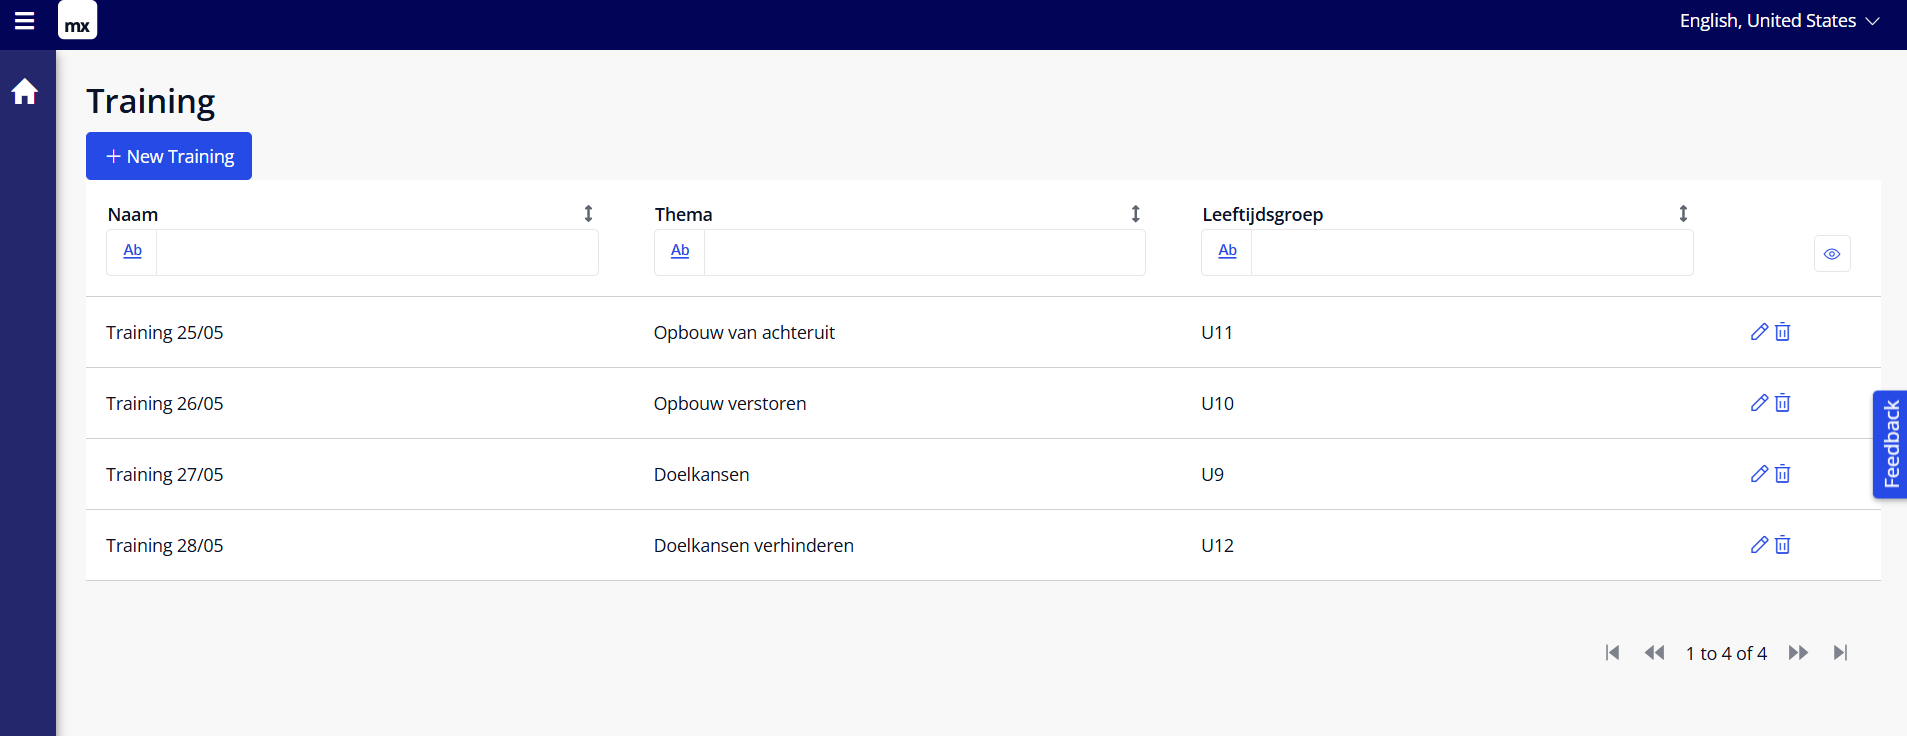
\includegraphics[width=0.8\textwidth]{Homepage-Mendix.png}
    \caption[Homepage Mendix applicatie]{\label{fig:homepage-mendix} Homepage Mendix applicatie }
\end{figure}

\begin{figure}[H]
    \centering
    \captionsetup{justification=centering}
    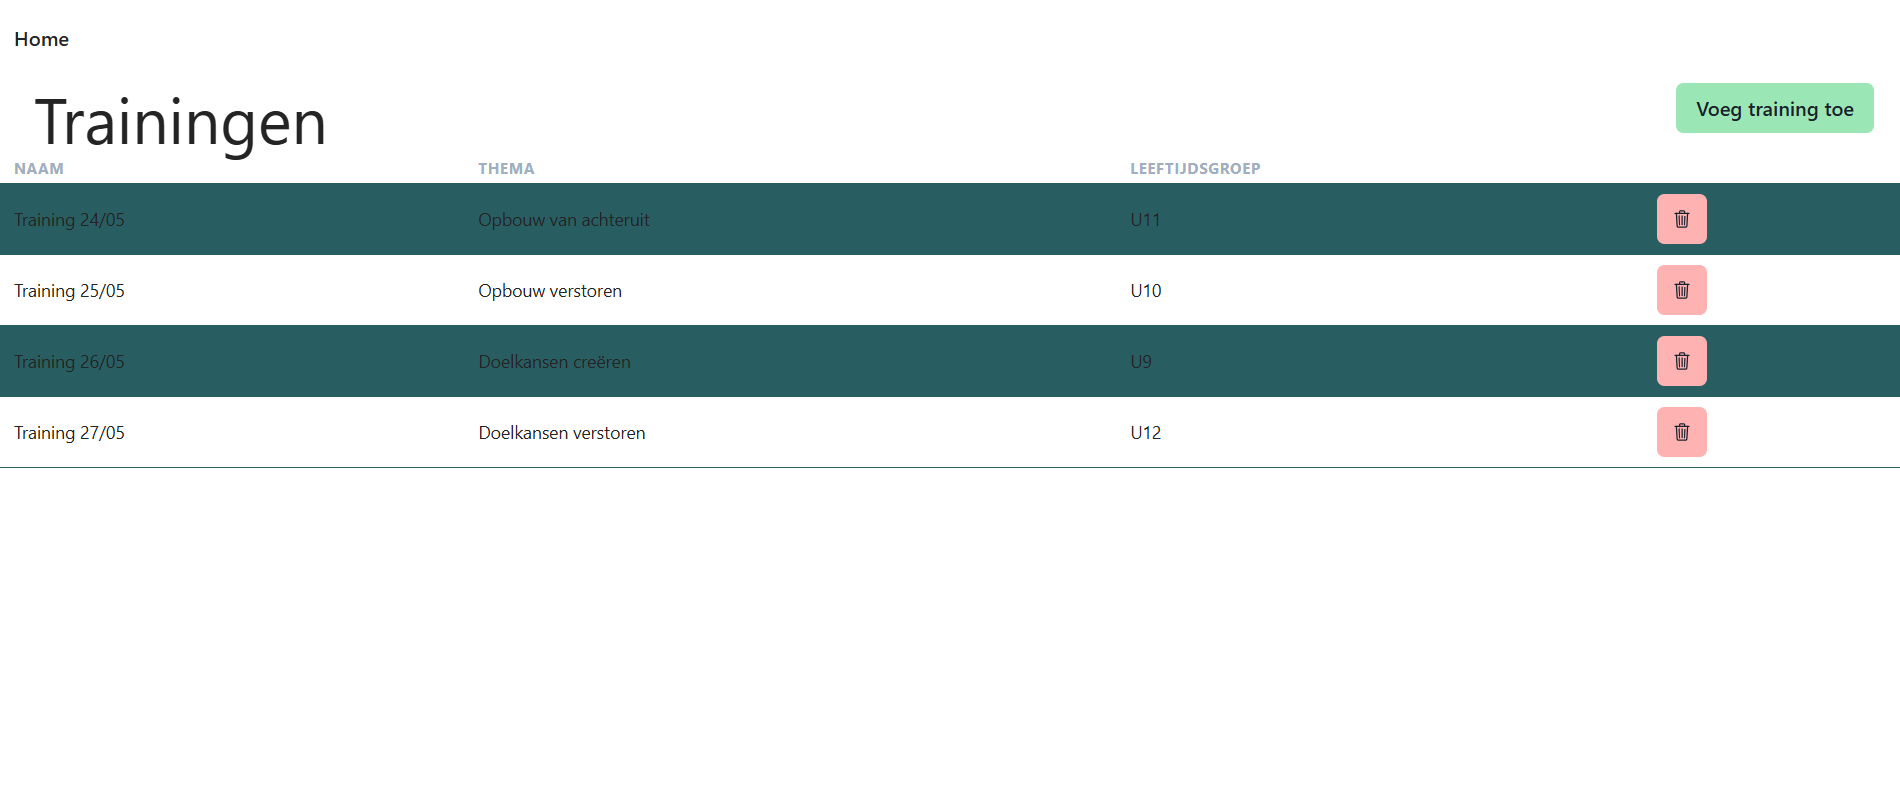
\includegraphics[width=0.8\textwidth]{Homepage-JS.png}
    \caption[Homepage Mendix applicatie]{\label{fig:homepage-JavaScript} Homepage JavaScript/React applicatie }
\end{figure}

Het doel van deze vergelijking is om inzicht te krijgen in de sterktes en beperkingen van beide technologieën op basis van praktijkgerichte criteria. De evaluatie richt zich op vijf hoofdgebieden: prestatie en schaalbaarheid, integratiemogelijkheden, aanpasbaarheid en uitbreidbaarheid, ontwikkelsnelheid en beveiliging en compliance. Voor elk van deze categorieën worden gerichte testen uitgevoerd, variërend van technische benchmarks (zoals laadtijd en load testing) tot ontwikkelervaring en gebruiksvriendelijkheid. Door beide applicaties op systematische wijze te testen, wordt duidelijk in welke scenario’s Mendix of juist een traditionele JavaScript/React-stack de voorkeur verdient. De resultaten uit deze vergelijking vormen de basis voor de uiteindelijke conclusie over de toepasbaarheid van beide benaderingen binnen diverse zakelijke contexten.
\subsection{Schaalbaarheid en prestaties}
Om een objectieve vergelijking te kunnen maken tussen de in Mendix en in JavaScript/React ontwikkelde applicaties, zijn verschillende prestatie- en schaalbaarheidstesten uitgevoerd. Deze testen richten zich op drie kernaspecten: de laadtijd van de applicatie, de reactietijd op gebruikersacties en de prestaties onder belasting. Voor het meten van de laadtijd zijn tools zoals Google Lighthouse en Chrome DevTools gebruikt, waarmee onder andere de \gls{FCP} en de \gls{LCP} zijn geanalyseerd. Daarnaast is de reactietijd op interacties met de gebruikersinterface gemeten om de responsiviteit van beide applicaties te beoordelen. Tot slot wordt een load test uitgevoerd met een tool, Apache JMeter, om inzicht te krijgen in de schaalbaarheid en het gedrag van de applicaties bij een hoge gebruikersbelasting. Deze metingen geven een duidelijk beeld van de praktische prestaties van beide technologieën in een realistische gebruiksomgeving.

\subsubsection{Laadtijd (Performance)}
De laadtijd van een webapplicatie is een cruciale factor voor de gebruikerservaring, aangezien gebruikers doorgaans verwachten dat een pagina binnen 2 à 3 seconden volledig geladen is. Om de prestaties van beide applicaties objectief te meten, werd gebruikgemaakt van Google Lighthouse. Deze tool analyseert verschillende web performance-indicatoren, waaronder:
\begin{itemize}
    \item \gls{FCP}
    \item \gls{LCP}
    \item \gls{TBT}
    \item Speed Index
    \item \gls{CLS}
    \item Performance Score (algemene score op 100)
\end{itemize}

\subsubsection{Resultaten}

Voor zowel de Mendix-applicatie als de JavaScript/React-applicatie werden telkens drie afzonderlijke metingen uitgevoerd. De resultaten van deze testen zijn gemiddeld om zo een eerlijke vergelijking te maken.
\newpage
\paragraph{JavaScript/React resultaten laadtijd}

\begin{table}[h]
    \centering
    \begin{tabular}{ |p{3cm}|p{2.75cm}|p{2.75cm}|p{2.75cm}|p{2.75cm}|}
        \hline
        \textbf{Metriek} & \textbf{Test 1} & \textbf{Test 2}  & \textbf{Test 3} & \textbf{Gemiddelde}\\
        \hline
        \textbf{\gls{FCP}}  & 11.8s & 11.8s & 11.7s & 11.8s \\
        \hline
        \textbf{\gls{LCP}} & 22.8s & 22.9s & 22.6s & 22.8s\\
        \hline
        \textbf{\gls{TBT}}  & 540ms & 610ms & 340ms & 497ms \\
        \hline
        \textbf{Speed Index}  & 11.8s & 11.8s & 11.7s & 11.8s \\
        \hline
        \textbf{\gls{CLS}}  & 0 & 0  & 0 & 0 \\
        \hline
        \textbf{Performance Score}  & 42 & 40  & 48 & 43 \\
        \hline
    \end{tabular}
    \caption[\centering Testresultaten laadtijd JavaScript/React]{\label{tab:Testresultaten JavaScript/React}Testresultaten JavaScript/React.}
\end{table}

\begin{figure}[htbp]
    \centering
    \captionsetup{justification=centering}
    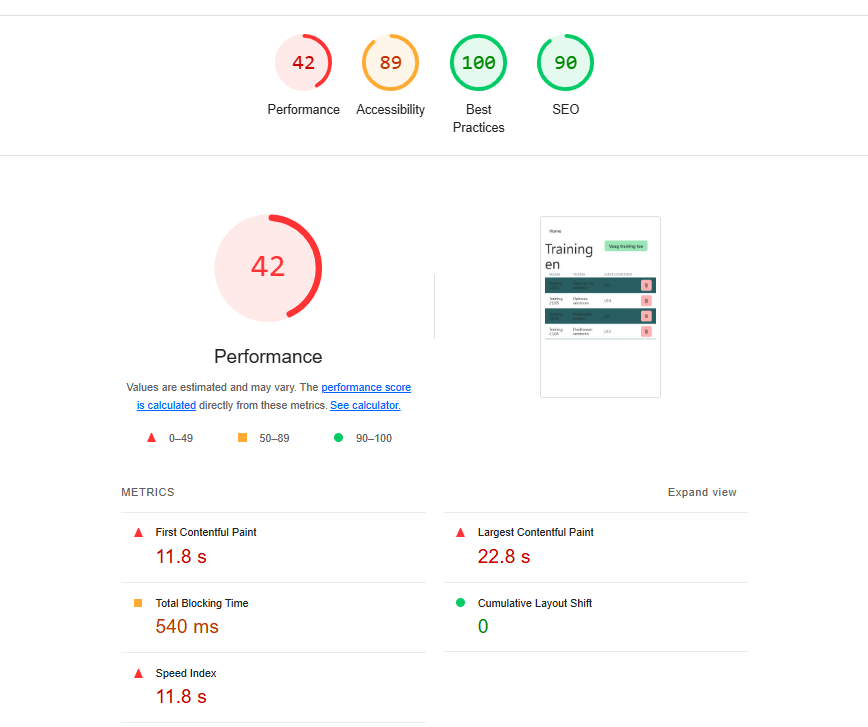
\includegraphics[width=0.3\textwidth]{JS-test1.png}
    \hfill
    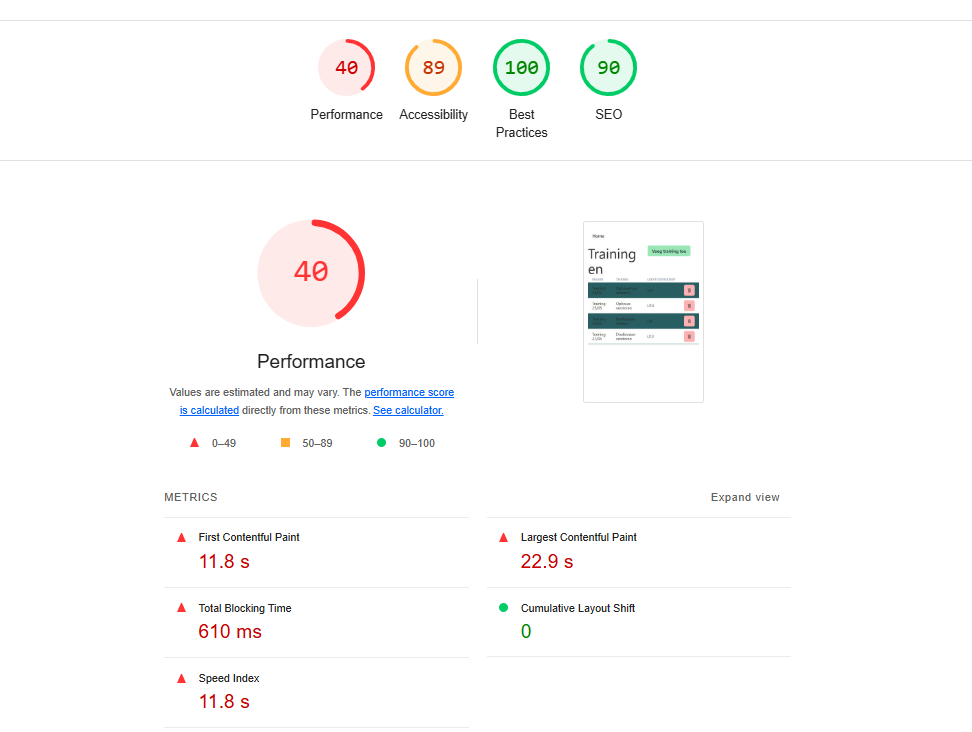
\includegraphics[width=0.3\textwidth]{JS-test2.png}
    \hfill
    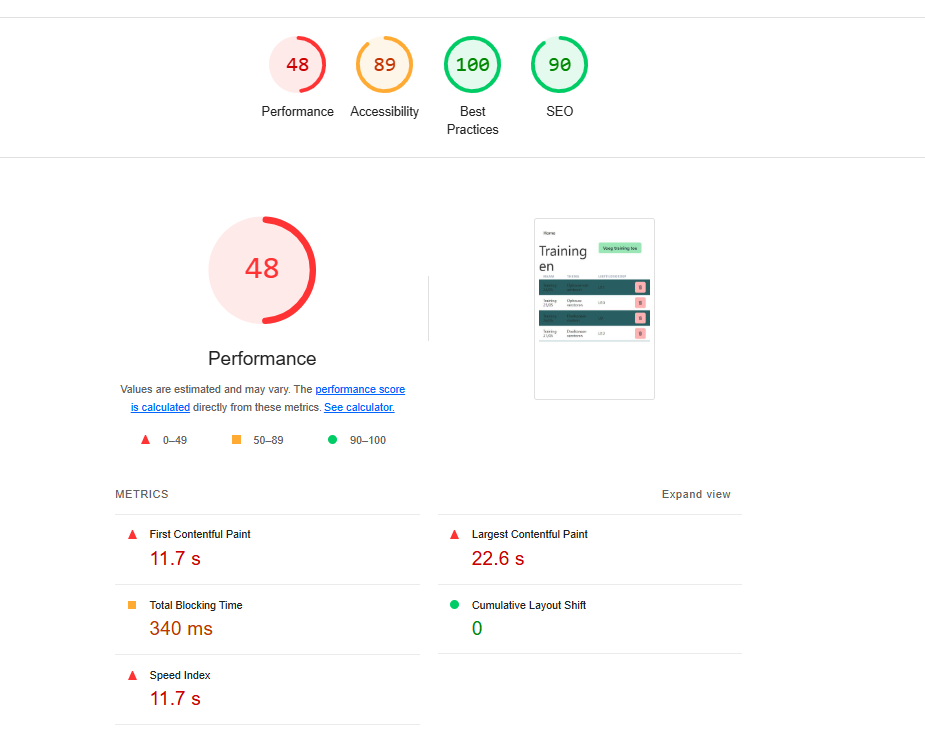
\includegraphics[width=0.3\textwidth]{JS-test3.png}
    \caption{Lighthouse testresultaten JavaScript/React - Links: Test 1, Midden: Test 2, Rechts: Test 3}
    \label{fig:javascript-simple}
\end{figure}

\newpage
\paragraph{Mendix resultaten laadtijd}

\begin{table}[h]
    \centering
    \begin{tabular}{ |p{3cm}|p{2.75cm}|p{2.75cm}|p{2.75cm}|p{2.75cm}|}
        \hline
        \textbf{Metriek} & \textbf{Test 1} & \textbf{Test 2}  & \textbf{Test 3} & \textbf{Gemiddelde}\\
        \hline
        \textbf{\gls{FCP}}  & 13.7s & 13.9s & 13.7s & 13.8s \\
        \hline
        \textbf{\gls{LCP}} & 17.8s & 18.2s & 17.8s & 17.9s\\
        \hline
        \textbf{\gls{TBT}}  & 330ms & 500ms & 260ms & 363ms \\
        \hline
        \textbf{Speed Index}  & 13.7s & 13.9s & 13.7s & 13.8s \\
        \hline
        \textbf{\gls{CLS}}  & 0 & 0  & 0 & 0 \\
        \hline
        \textbf{Performance Score}  & 48 & 43  & 50 & 47 \\
        \hline
    \end{tabular}
    \caption[\centering Testresultaten laadtijd Mendix]{\label{tab:Testresultaten Mendix}Testresultaten Mendix}
\end{table}

\begin{figure}[htbp]
    \centering
    \captionsetup{justification=centering}
    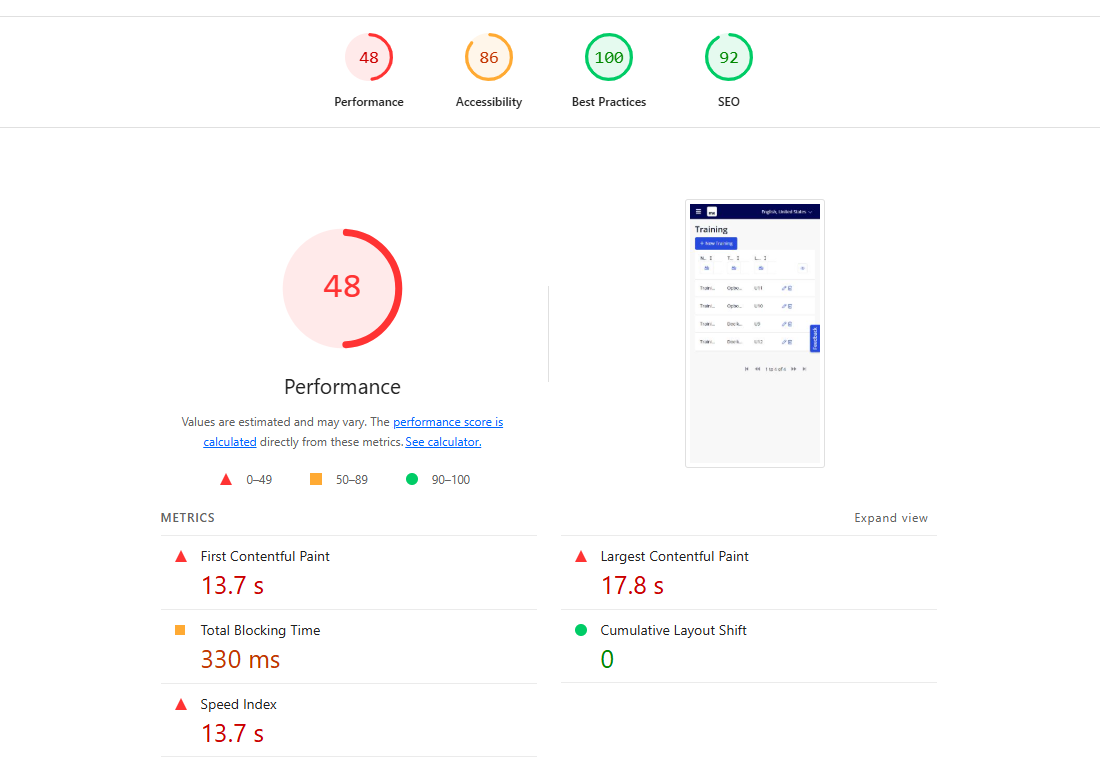
\includegraphics[width=0.3\textwidth]{Mendix-test1.png}
    \hfill
    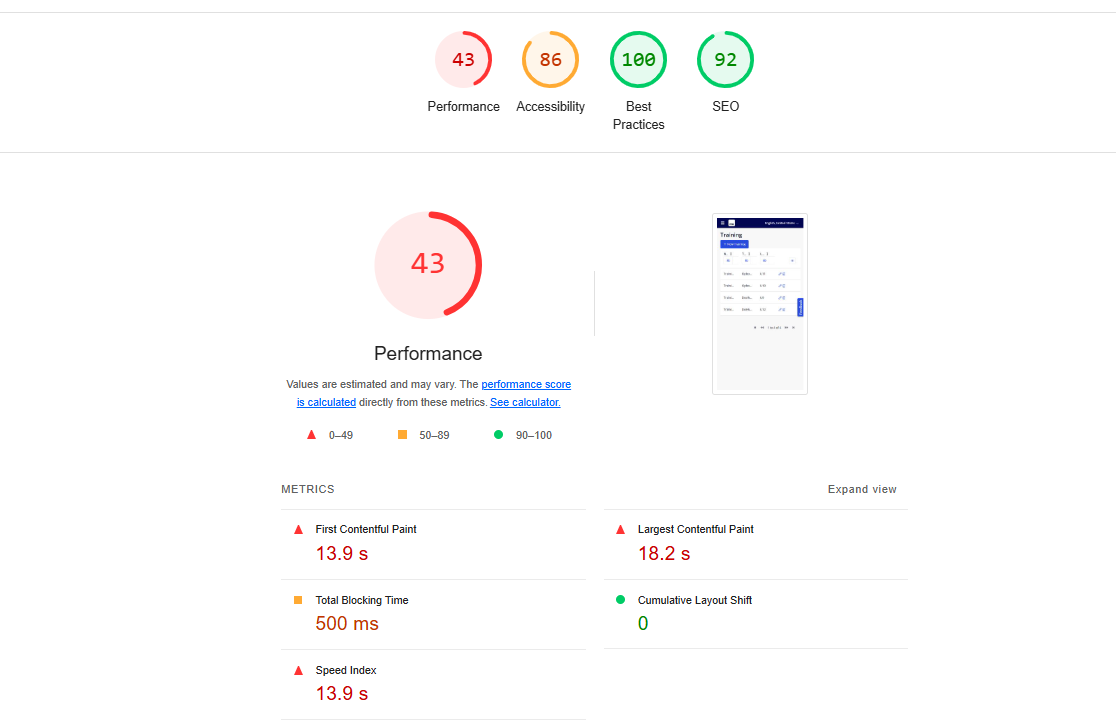
\includegraphics[width=0.3\textwidth]{Mendix-test2.png}
    \hfill
    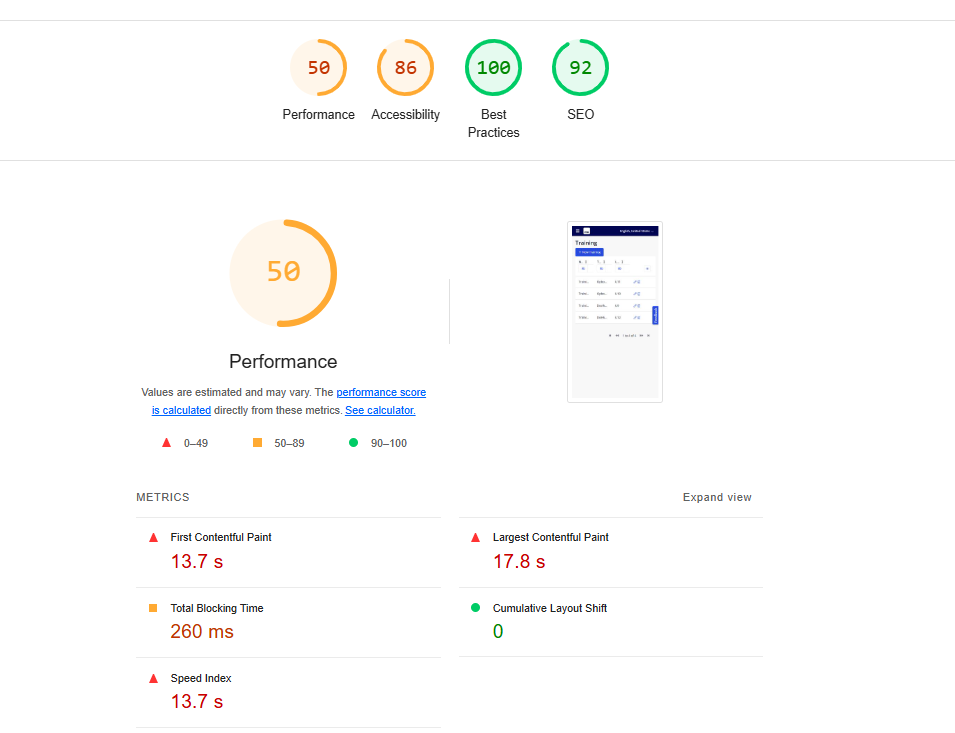
\includegraphics[width=0.3\textwidth]{Mendix-test3.png}
    \caption{Lighthouse testresultaten Mendix - Links: Test 1, Midden: Test 2, Rechts: Test 3}
    \label{fig:mendix-simple}
\end{figure}
\newpage
\paragraph{Vergelijkingstabel}
\begin{table}[h]
    \centering
    \begin{tabular}{ |p{3cm}|p{2.25cm}|p{2.25cm}|p{2.25cm}|p{3.25cm}|}
        \hline
        \textbf{Metriek} & \textbf{JavaScript/} \newline \textbf{React} & \textbf{Mendix}  & \textbf{Verschil} & \textbf{Beste Prestatie}\\
        \hline
        \textbf{\gls{FCP}}  & 11.8s & 13.8s & -2.0s & JavaScript/React \\
        \hline
        \textbf{\gls{LCP}} & 22.8s & 17.8s & +4.9s & Mendix\\
        \hline
        \textbf{\gls{TBT}}  & 497ms & 363ms & +134ms & Mendix \\
        \hline
        \textbf{Speed Index}  & 11.8s & 13.8s & -2.0s & JavaScript/React \\
        \hline
        \textbf{\gls{CLS}}  & 0 & 0  & Gelijk & Gelijk \\
        \hline
        \textbf{Performance Score}  & 43 & 47  & -4 & Mendix \\
        \hline
    \end{tabular}
    \caption[\centering Vergelijkingstabel laadtijd]{\label{tab:Vergelijkingstabel laadtijd}Vergelijkingstabel laadtijd}
\end{table}

\paragraph{Samenvatting}
\begin{itemize}
    \item JavaScript/React is sneller bij \gls{FCP} en Speed Index (2s sneller)
    \item Mendix presteert beter bij \gls{LCP} (4,9s sneller) en \gls{TBT} (134ms minder)
    \item Mendix heeft een hogere Performance Score (47 vs 43)
    \item Beide platforms hebben perfecte \gls{CLS} scores
    \item Beide platforms scoren onder acceptabele performance niveaus (<50)
\end{itemize}
De prestatieverschillen tussen Mendix en JavaScript/React kunnen verklaard worden door fundamentele verschillen in architectuur en uitvoering. JavaScript/React scoort beter op \gls{FCP} doordat het doorgaans gebruikmaakt van een lichte initiële bundel en client-side rendering, waardoor visuele elementen snel zichtbaar zijn. Mendix presteert daarentegen beter op \gls{LCP} en \gls{TBT} dankzij de geïntegreerde backend, geoptimaliseerde dataverwerking en beperkte client-side JavaScript. Door logica server-side af te handelen en automatisch platformoptimalisaties toe te passen, vermindert Mendix de belasting op de browser, wat resulteert in betere prestaties bij het laden van grote elementen en minder blokkeringen tijdens interacties.

\subsubsection{Reactietijd op gebruikersacties}
De reactietijd van een webapplicatie is de tijd tussen een gebruikersactie (zoals een klik) en het zichtbare resultaat. Deze reactietijd is essentieel voor een vloeiende gebruikerservaring. Gebruikers verwachten dat interacties vrijwel onmiddellijk reageren, idealiter binnen 100 tot 200 milliseconden. Om de reactietijd objectief te evalueren, werd een handmatige performance-analyse uitgevoerd met behulp van de ontwikkelaarstools in Google Chrome (Performance tab). 

\subsubsection{Resultaten}
Bij de testen werd specifiek gekeken naar het toevoegen van een nieuw item binnen zowel de Mendix- als de JavaScript/React-applicatie. Door de belangrijkste fasen van dit proces in kaart te brengen, van het moment waarop een gebruiker een actie uitvoert tot aan de visuele terugkoppeling op het scherm, kon een nauwkeurige vergelijking worden gemaakt van de snelheid en efficiëntie van beide implementaties.

\paragraph{JavaScript/React resultaten reactietijd}

\begin{figure}[H]
    \centering
    \captionsetup{justification=centering}
    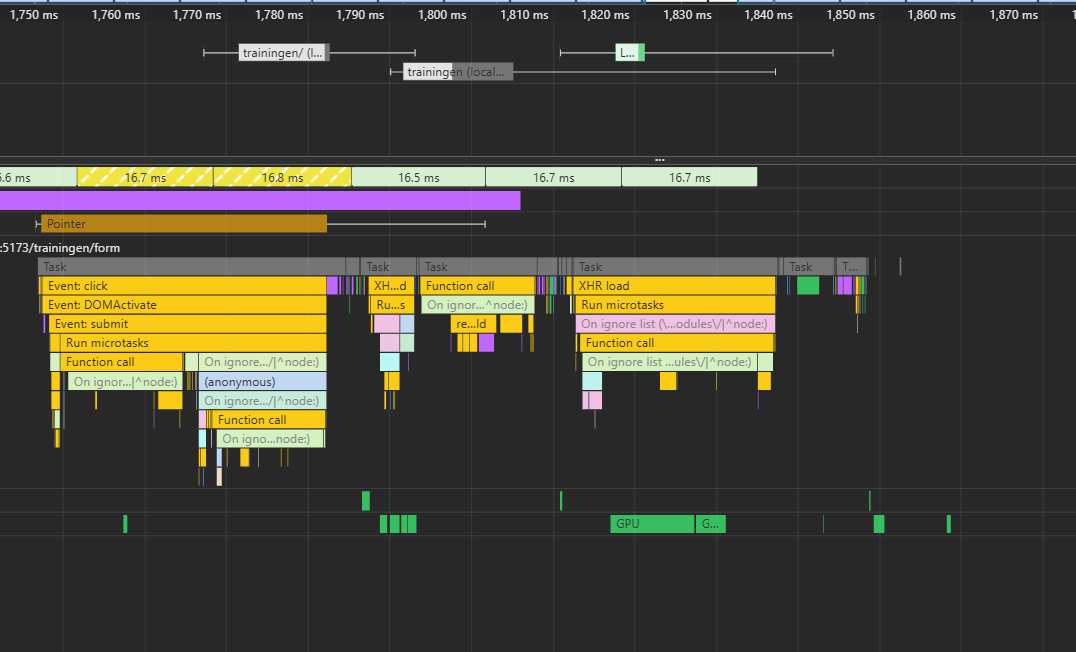
\includegraphics[width=0.8\textwidth]{Test JS reactietijd Toevoegen.png}
    \caption[Testresultaten toevoegen object in JavaScript/React]{\label{fig:reactietijd-JavaScript} Testresultaten toevoegen object in JavaScript/React }
\end{figure}


\begin{table}[H]
    \centering
    \begin{tabular}{ |p{4cm}|p{3cm}|p{6cm}|p{1cm}|}
        \hline
        \textbf{Metriek} & \textbf{Tijd/Duur} & \textbf{Beschrijving} & \textbf{Fase}\\
        \hline
        \textbf{Start operatie/ Event Click}  & $\sim$1.750 ms & Start van gebruikersinteractie & 1\\
        \cline{1-3}
        \textbf{\gls{DOM} Activate} & $\sim$1.752 ms & Verwerking van DOM-event &  \\
        \cline{1-3}
        \textbf{Event Submit}  & $\sim$1.754 ms & Formulier wordt verstuurd &  \\
        \cline{1-3}
        \textbf{Microtasks}  & 1.754 – 1.756 ms & Uitvoering van JavaScript-taken &  \\
        \hline                       
        \textbf{\gls{XHR} Load}  & 1.790 – 1.820 ms & Communicatie met de server & 2 \\
        \hline
        \textbf{Function Calls}  & 1.820 – 1.840 ms & Verwerking van de serverrespons & 3 \\
        \hline
        \textbf{GPU Rendering}  & $\sim$1.850 ms & 	Visuele weergave (rendering) & 4 \\
        \hline
        \textbf{Reactietijd}  & ≈ 100 ms & 	Tijdsduur van klik tot weergave & 1,2,3,4 \\
        \hline
    \end{tabular}
    \caption[\centering Testresultaten reactietijd JavaScript/React]{\label{tab:Testresultaten JS reactietijd}Testresultaten reactietijd JavaScript/React}
\end{table}

\begin{table}[H]
    \centering
    \begin{tabular}{ |p{5,5cm}|p{3cm}|p{6cm}|}
        \hline
        \textbf{Fase} & \textbf{Duur} & \textbf{Activiteit}\\
        \hline
        \textbf{1. Eventverwerking}  & $\sim$4 ms & Van klik tot submit \\
        \hline
        \textbf{2. \gls{XHR}-verzoek} & $\sim$30 ms & Verzoek naar en antwoord van de server \\
        \hline
        \textbf{3. Responsverwerking}  & $\sim$20 ms & Verwerking van ontvangen data \\
        \hline
        \textbf{4. Visuele rendering}  & $\sim$46 ms & \gls{UI} wordt bijgewerkt op het scherm \\
        \hline                       

    \end{tabular}
    \caption[\centering Breakdown reactietijd JavaScript/React]{\label{tab:breakdown JS reactietijd}Breakdown reactietijd JavaScript/React}
\end{table}



\newpage




\paragraph{Mendix resultaten reactietijd}

\begin{figure}[H]
    \centering
    \captionsetup{justification=centering}
    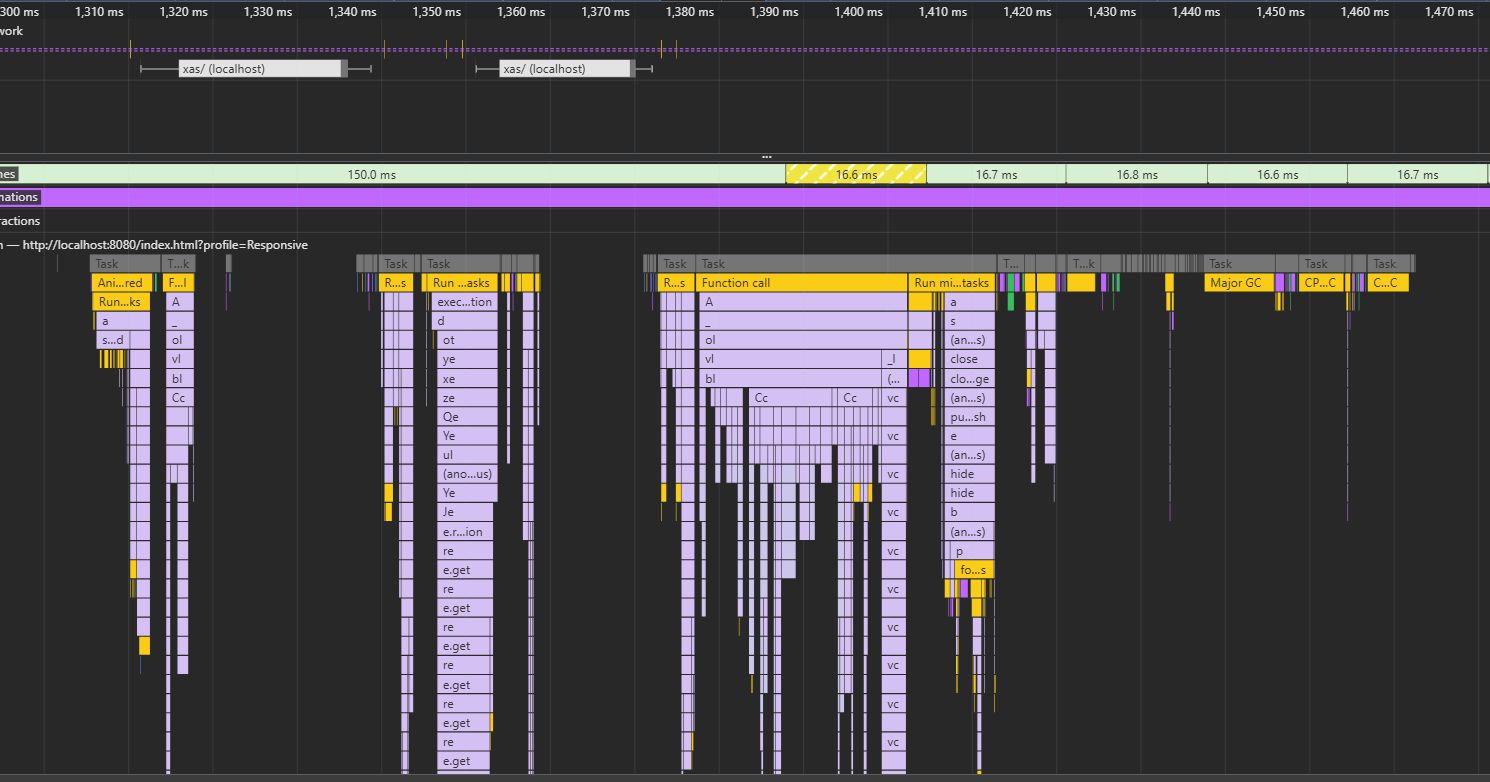
\includegraphics[width=0.8\textwidth]{Test Mendix reactietijd Toevoegen.png}
    \caption[Testresultaten toevoegen object in Mendix]{\label{fig:reactietijd-Mendix} Testresultaten toevoegen object in Mendix}
\end{figure}


\begin{table}[H]
    \centering
    \begin{tabular}{|p{4cm}|p{3cm}|p{6cm}|p{1cm}|}
        \hline
        \textbf{Metriek}   & \textbf{Tijd/Duur} & \textbf{Beschrijving} & \textbf{Fase} \\
        \hline
        \textbf{Start operatie} & $\sim$1.300 ms & Start van gebruikersinteractie & 1 \\
        \cline{1-3}
        \textbf{Animation/Render} & 1.300 - 1.320 ms & \gls{UI} animaties enrendering & \\
        \hline
        \textbf{Run Tasks} & 1.320 - 1.340 ms & Asynchrone task verwerking & 2 \\
        \hline
        \textbf{Function Calls} & 1.340 - 1.380 ms & Core applicatie logica & 3 \\
        \hline                       
        \textbf{Major \gls{GC}} & 1.790 – 1.820 ms & Communicatie met de server & 4 \\
        \cline{1-3}
        \textbf{Function Calls} & 	$\sim$1.440 ms & Garbage collection & \\
        \cline{1-3}
        \textbf{Operatie Compleet} & $\sim$1.470 ms & 	Item volledig toegevoegd & \\
        \hline
        \textbf{Totale reactietijd} &  ≈ 170 ms & Tijdsduur van klik tot weergave & 1,2,3,4 \\
        \hline
    \end{tabular}
    \caption[\centering Testresultaten reactietijd Mendix]{\label{tab:Testresultaten Mendix reactietijd}Testresultaten reactietijd Mendix}
\end{table}

\begin{table}[H]
    \centering
    \begin{tabular}{|p{5,5cm}|p{3cm}|p{6cm}|}
        \hline
        \textbf{Fase} & \textbf{Duur} & \textbf{Activiteit}\\
        \hline
        \textbf{1. Initial Animation}  & $\sim$20 ms & \gls{UI} feedback start \\
        \hline
        \textbf{2. Task Processing} & $\sim$20 ms & Asynchrone verwerking \\
        \hline
        \textbf{3. Function Execution}  & $\sim$40 ms & Business logica \\
        \hline
        \textbf{4. Rendering and \gls{GC}}  & $\sim$90 ms & \gls{UI} updates + cleanup \\
        \hline                       
        
    \end{tabular}
    \caption[\centering Breakdown reactietijd Mendix]{\label{tab:breakdown Mendix reactietijd}Breakdown reactietijd Mendix}
\end{table}


\pagebreak
\newpage


\paragraph{Conclusie}
Hoewel JavaScript met 100 ms iets sneller is dan Mendix met 170 ms van start tot completion, is het verschil van 70 ms relatief klein en valt het binnen een categorie van zeer responsieve prestaties. JavaScript profiteert van snellere verwerking, maar omvat ook een server roundtrip van ongeveer 30 ms via \gls{XHR} calls, terwijl Mendix juist meer lokale verwerking en \gls{GC} uitvoert, wat zorgt voor extra framework overhead. Beide platformen tonen vergelijkbare tijden voor de kernlogica (~50-60 ms), wat aangeeft dat het verschil vooral zit in de \gls{UI} rendering en framework processing. Voor een kleine applicatie is deze lichte vertraging in Mendix een acceptabele trade-off, gezien de rijkere functionaliteit en gebruikerservaring die het biedt. Bij grotere en complexere applicaties kan de Mendix overhead echter toenemen, wat de prestaties meer beïnvloedt. Desondanks leveren beide technologieën een vrijwel directe respons die gebruikers als “instant” ervaren, waardoor deze realistische vergelijking een eerlijk beeld geeft van de praktische prestaties in echte toepassingen.



\subsubsection{Load test}
Om de schaalbaarheid en robuustheid van de webapplicaties te evalueren onder verschillende belastingniveaus, werden ook loadtesten uitgevoerd. Deze testen simuleren een toenemend aantal gelijktijdige gebruikers om te bepalen hoe de applicaties presteren onder stress en om eventuele knelpunten te identificeren.

\subsubsection{Resultaten}
De loadtesten zijn uitgevoerd door het simuleren van HTTP-verzoeken voor een oplopend aantal gebruikers (10, 100, 250, 500, 1000, 2500 gebruikers) voor zowel de Mendix- als de JavaScript/React-applicatie. Hierbij is gebruikgemaakt van Apache JMeter, een veelgebruikte tool voor het uitvoeren van prestatietests, waarmee realistische gebruikersinteracties kunnen worden nagebootst. De belangrijkste metingen die zijn geanalyseerd, omvatten de gemiddelde reactietijd, het aantal requests per seconde (throughput) en het foutpercentage (Error \%).

\paragraph{JavaScript/React resultaten load testen}

\begin{figure}[H]
    \centering
    \captionsetup{justification=centering}
    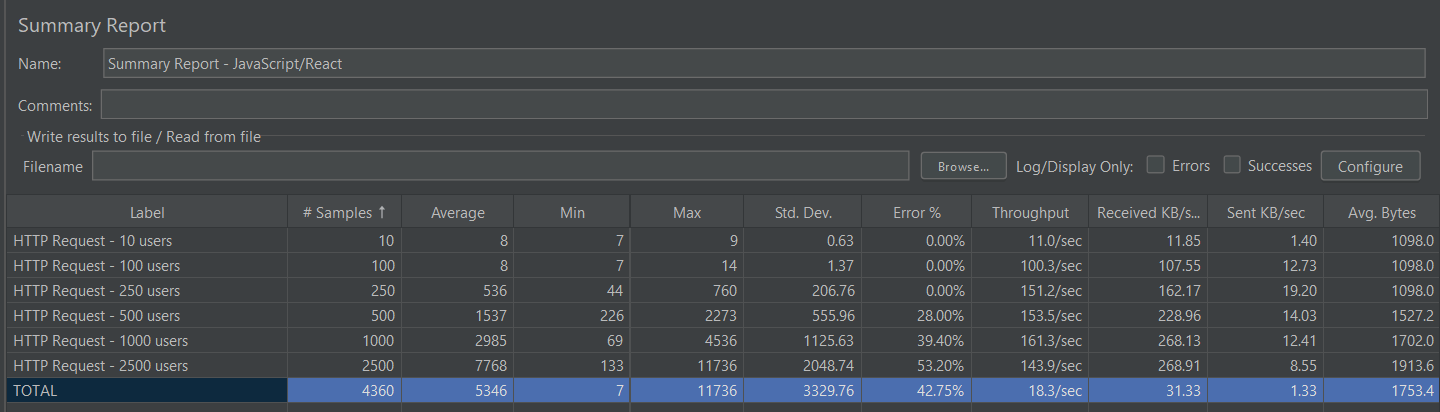
\includegraphics[width=0.8\textwidth]{Test JS load.png}
    \caption[\centering Testresultaten load test: ophalen objecten in JavaScript/React]{\label{fig:loadtest-JavaScript} Testresultaten load test: ophalen objecten in JavaScript/React}
\end{figure}


\begin{table}[h]
    \centering
    \begin{tabular}{ |p{5cm}|p{3cm}|p{3cm}|p{3cm}|}
        \hline
        \textbf{Aantal gelijktijdige \newline gebruikers} & \textbf{Gemiddelde reactietijd (ms)} & \textbf{Error \newline percentage (\%)} & \textbf{Throughput (requests/sec)}\\
        \hline
        \textbf{10}  & 8 & 0.00 & 11.0 \\
        \hline
        \textbf{100} & 8 & 0.00 & 100.3 \\
        \hline
        \textbf{250}  & 536 & 0.00 & 151.2 \\
        \hline
        \textbf{500}  & 1537 & 28.00 & 153.5 \\
        \hline                       
        \textbf{1000}  & 2985 & 39.40 & 161.3  \\
        \hline
        \textbf{2500}  & 7768 & 53.20 & 143.9 \\
        \hline
    \end{tabular}
    \caption[\centering Loadtestresultaten JavaScript/React: Kernmetrieken]{\label{tab:Testresultaten JS loadtest}Loadtestresultaten JavaScript/React: Kernmetrieken}
\end{table}


\paragraph{Mendix resultaten load testen}

\begin{figure}[H]
    \centering
    \captionsetup{justification=centering}
    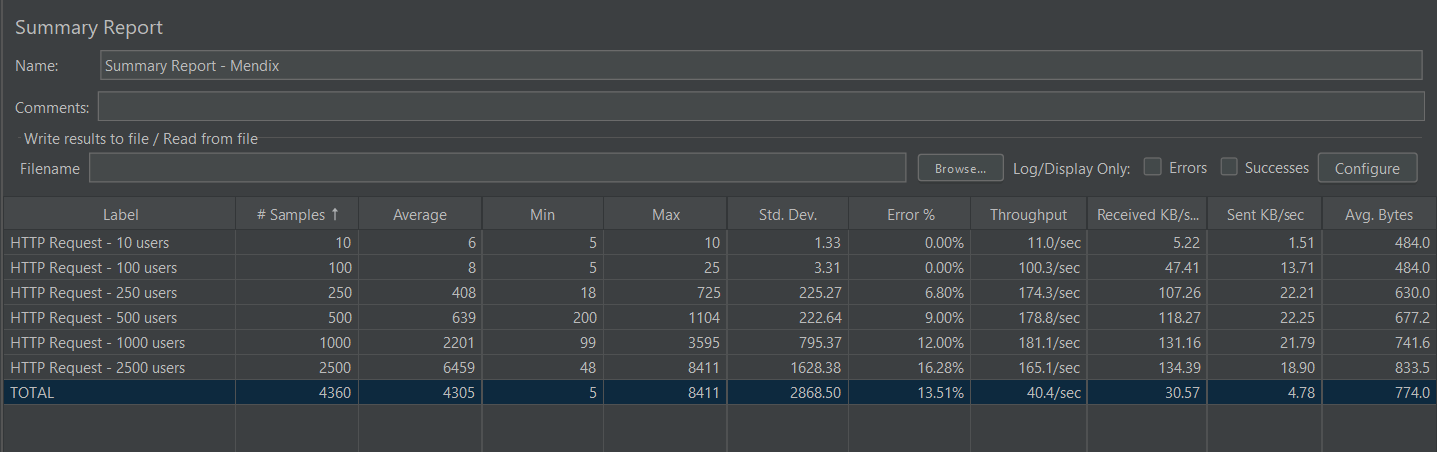
\includegraphics[width=0.8\textwidth]{Test load Mendix.png}
    \caption[\centering Testresultaten load test: ophalen objecten in Mendix]{\label{fig:loadtest-Mendix} Testresultaten load test: ophalen objecten in Mendix}
\end{figure}


\begin{table}[h]
    \centering
    \begin{tabular}{ |p{5cm}|p{3cm}|p{3cm}|p{3cm}|}
        \hline
        \textbf{Aantal gelijktijdige \newline gebruikers} & \textbf{Gemiddelde reactietijd (ms)} & \textbf{Error \newline percentage (\%)} & \textbf{Throughput (requests/sec)}\\
        \hline
        \textbf{10}  & 6 & 0.00 & 11.0 \\
        \hline
        \textbf{100} & 8 & 0.00 & 100.3 \\
        \hline
        \textbf{250}  & 408 & 6.80 & 174.3 \\
        \hline
        \textbf{500}  & 639 & 9.00 & 178.8 \\
        \hline                       
        \textbf{1000}  & 2201 & 12.00 & 181.1  \\
        \hline
        \textbf{2500}  & 6459 & 16.28 & 165.1 \\
        \hline
    \end{tabular}
    \caption[\centering Loadtestresultaten Mendix: Kernmetrieken]{\label{tab:Testresultaten Mendix loadtest}Loadtestresultaten Mendix: Kernmetrieken}
\end{table}



\paragraph{Conclusie}
Hoewel een JavaScript/React-applicatie theoretisch het potentieel heeft om Mendix te overtreffen in absolute prestaties, blijkt dit in de huidige load-testscenario’s niet het geval onder verhoogde belasting. Waar React flexibiliteit en volledige controle biedt voor optimalisatie, vereist dit ook aanzienlijke expertise en afstemming om daadwerkelijk robuust te blijven bij hoge gelijktijdige gebruikersaantallen. In de praktijk toont Mendix zich in deze tests stabieler, met name op het gebied van foutafhandeling en consistentie bij toenemende load. Dit is te danken aan de platformgebonden optimalisaties, standaardisatie en ingebouwde schaalbaarheidsmechanismen.

Beide technologieën hebben dus hun sterktes: Mendix excelleert in betrouwbaarheid en voorspelbaarheid bij grotere gebruikersvolumes, terwijl JavaScript/React (indien zorgvuldig geoptimaliseerd) de mogelijkheid biedt tot betere piekprestaties. De keuze hangt dan ook sterk af van de context en prioriteiten: snelle ontwikkeltrajecten met robuuste baseline-prestaties (Mendix) tegenover maximale flexibiliteit en performancepotentieel met meer technische investering (JavaScript/React). In de geteste scenario’s levert Mendix momenteel het meest consistente gedrag onder druk, wat voor veel toepassingen een doorslaggevend voordeel kan zijn.


\subsection{Ontwikkelsnelheid en onderhoud}

\subsubsection{Ontwikkeltijd}
De ontwikkeltijd is handmatig bijgehouden voor beide applicaties om een realistische inschatting te geven van de benodigde inspanning. Voor de JavaScript/React-applicatie bedroeg de totale ontwikkeltijd ongeveer 5 uur, waarbij tijd werd besteed aan het opzetten van de ontwikkelomgeving, het schrijven van de logica, het afhandelen van \gls{API}-calls, en het bouwen van de gebruikersinterface. Voor de Mendix-applicatie daarentegen was slechts 30 minuten nodig om een functioneel equivalent te realiseren. Deze aanzienlijke tijdwinst is te verklaren door het gebruik van vooraf gedefinieerde componenten, visuele modellering en standaardfunctionaliteit binnen het Mendix-platform. Hoewel JavaScript/React meer flexibiliteit en controle biedt, vereist het ook meer technische expertise en ontwikkelinspanning. Mendix blijkt in dit opzicht bijzonder efficiënt voor het snel realiseren van functionele prototypes of standaardapplicaties.

\subsubsection{Herbruikbaarheid / uitbreidbaarheid}
Om de aanpasbaarheid en herbruikbaarheid van componenten te evalueren, is bij beide applicaties een zoekfunctie toegevoegd. Dit biedt inzicht in hoe snel en flexibel nieuwe functionaliteit kan worden geïntegreerd. In Mendix kon de zoekfunctionaliteit in slechts 1 minuut worden geactiveerd door een bestaande zoekoptie in het component eenvoudig aan te zetten via de modeler-interface, een handeling die letterlijk neerkomt op het selecteren van een checkbox. 

\begin{figure}[H]
    \centering
    \captionsetup{justification=centering}
    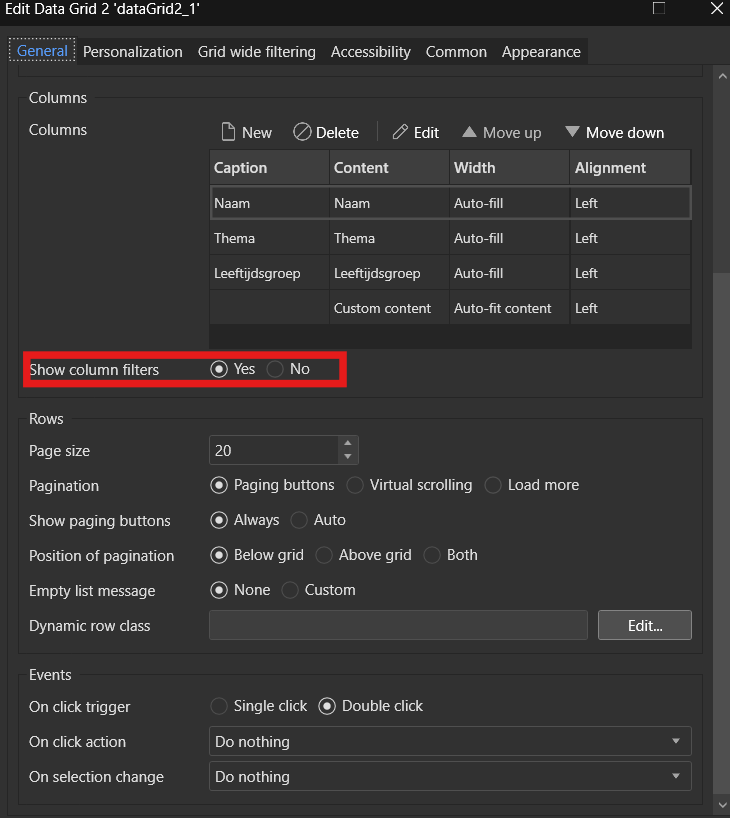
\includegraphics[width=0.5\textwidth]{show colomn filters.png}
    \caption[\centering Checkbox aanzetten filters]{\label{fig:show-colomn-filters-Mendix} Checkbox aanzetten filters}
\end{figure}


\begin{figure}[H]
    \centering
    \captionsetup{justification=centering}
    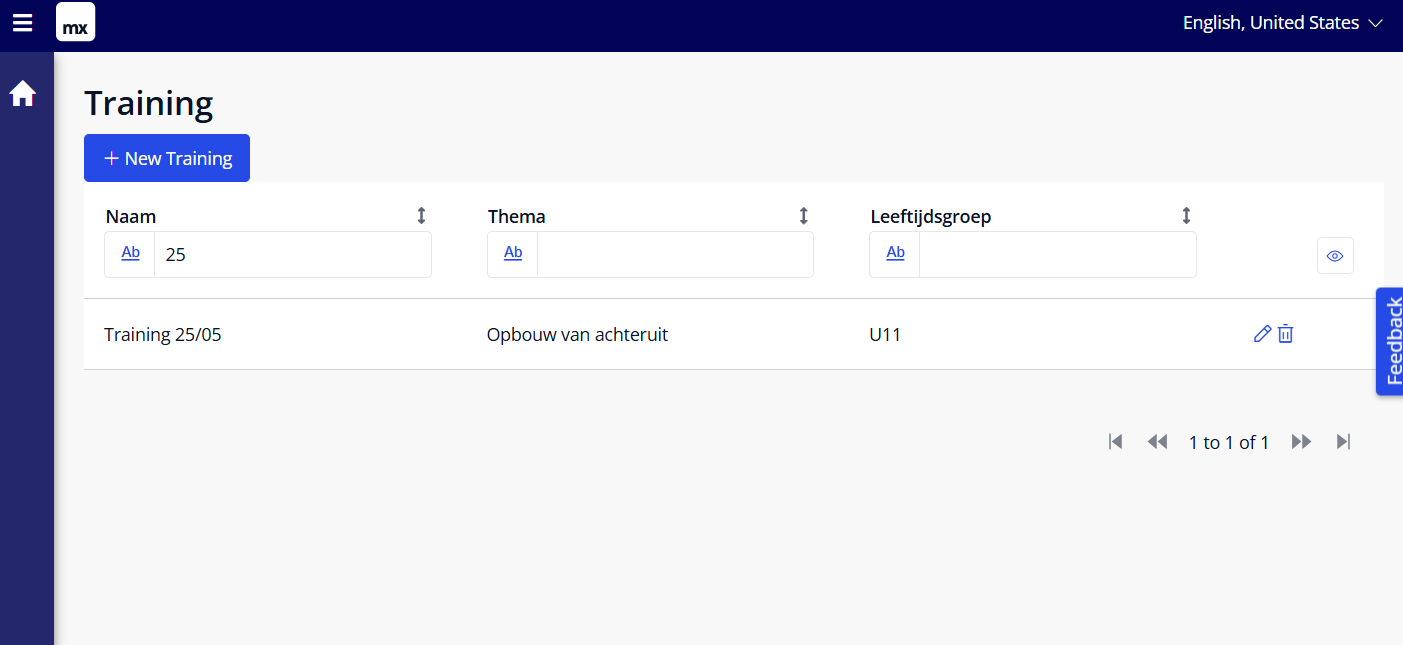
\includegraphics[width=1\textwidth]{Homepage with search Mendix.png}
    \caption[\centering Homepage with search bar]{\label{fig:homepage-with-search-Mendix} Homepage met zoekbalk Mendix}
\end{figure}



In JavaScript/React duurde het toevoegen van een vergelijkbare zoekfunctie ongeveer 15 minuten, waarbij logica handmatig moest worden geschreven, de zoekinput geïntegreerd diende te worden in de UI, en filtering op de dataset geïmplementeerd werd.

\begin{listing}[H]
    \begin{minted}{JavaScript}
export default function TrainingsTable({ trainingen, onDelete }) {
 const [searchTerm, setSearchTerm] = useState("");
 // Filter trainingen op basis van zoekterm
 const filteredTrainingen = trainingen.filter((training) =>
   training.naam.toLowerCase().includes(searchTerm.toLowerCase())
 );
 return (
  <Box>
  {/* Zoekbalk */}
  <Input
   placeholder="Zoek op naam..."
   value={searchTerm}
   onChange={(e) => setSearchTerm(e.target.value)}
   mb={4}
   maxWidth="300px"
  />
  {/* Tabel */}
  <Table variant="striped" colorScheme="teal" size="sm">
    <Thead>
      <Tr>
        <Th>Naam</Th>
        <Th>Thema</Th>
        <Th>Leeftijdsgroep</Th>
        <Th></Th>
      </Tr>
    </Thead>
    <Tbody>
      {filteredTrainingen.length > 0 ? (filteredTrainingen.map((training) => (
        <Training key={training.id} onDelete={onDelete} {...training} />)))}
    </Tbody>
  </Table>
 </Box>
 );
}   
    \end{minted}
    \captionsetup{justification=centering}
    \caption{Trainingstabel met zoekfunctie op naam}
    \label{lst:pipeline-clone}
\end{listing}

\begin{figure}[H]
    \centering
    \captionsetup{justification=centering}
    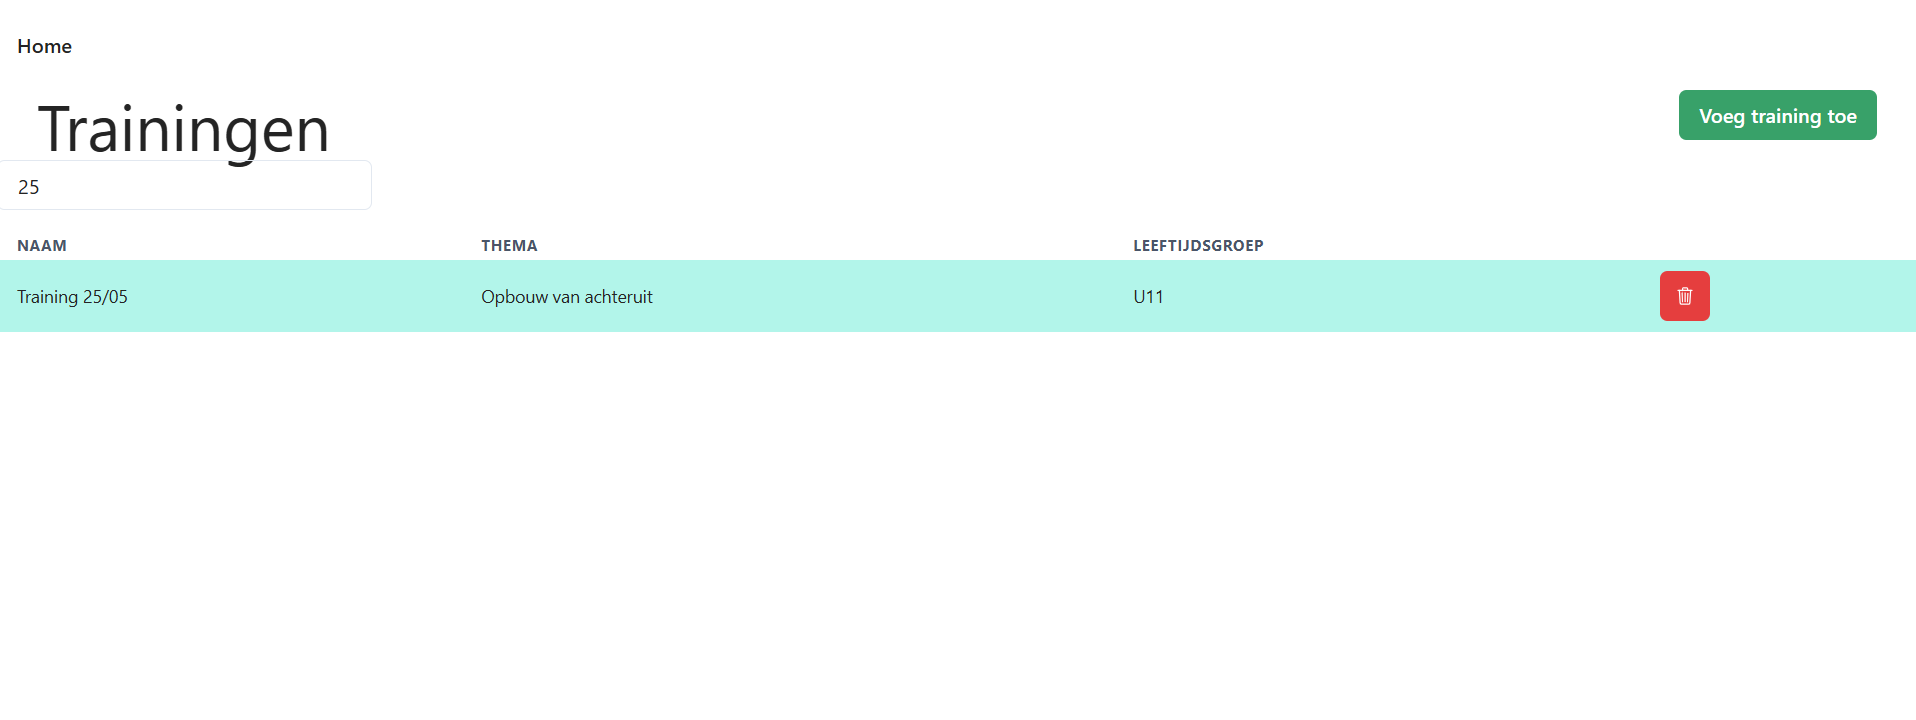
\includegraphics[width=1\textwidth]{Homepage with search JS.png}
    \caption[\centering Homepage with search bar JavaScript/React]{\label{fig:homepage-with-search-JS} Homepage met zoekbalk JavaScript/React}
\end{figure}


 Hoewel de implementatie in beide gevallen vlot verliep, toont dit voorbeeld aan dat Mendix dankzij herbruikbare en vooraf geconfigureerde componenten bijzonder efficiënt is bij het uitbreiden van functionaliteit, terwijl JavaScript/React meer flexibiliteit biedt maar ook meer ontwikkelwerk vraagt.


\subsection{Integratiemogelijkheden}

Zowel Mendix als JavaScript/React bieden uitgebreide mogelijkheden om te integreren met externe systemen. De manier waarop deze integraties tot stand komen verschilt aanzienlijk vanwege hun aard: Mendix als low-code platform en JavaScript/React als code-first benadering.

\subsubsection{Mendix}

Mendix is ontworpen om eenvoudig te koppelen met zowel moderne als legacy systemen, met standaard ondersteuning voor verschillende integratietechnieken:
\begin{itemize}
    \item \textbf{REST \gls{API}'s}: volledige ondersteuning voor het bouwen en consumeren van RESTful APIs. Integraties zoals met Salesforce of SAP zijn vlot op te zetten via visuele flows.
    \item \textbf{SOAP Webservices}: ondersteuning voor oudere protocollen blijft behouden, wat belangrijk is voor bedrijven met legacy infrastructuren.
    \item \textbf{GraphQL}: niet native ondersteund, maar via extensies of community-modules kunnen GraphQL-endpoints alsnog worden aangesproken.
    \item \textbf{OData Services}: Mendix biedt OData-integraties voor onder meer BI-tools zoals Power BI.
    \item \textbf{Databaseconnecties}: directe verbinding met relationele databases zoals SQL Server, MySQL, PostgreSQL en Oracle.
\end{itemize}

Daarnaast is er toegang tot Mendix Connect en de Mendix Marketplace, waar herbruikbare connectors beschikbaar zijn voor populaire systemen zoals SAP, Salesforce, Kafka en meer. Dit maakt het voor ontwikkelaars mogelijk om snel integraties op te zetten zonder complexe code.

\subsubsection{JavaScript/React}

JavaScript/React biedt in essentie volledige vrijheid voor integratie, maar dit betekent ook dat ontwikkelaars zelf verantwoordelijk zijn voor de implementatie van alle benodigde logica en security rond die integraties:
\begin{itemize}
    \item \textbf{REST en GraphQL}: beide worden uitstekend ondersteund via moderne bibliotheken zoals Axios, Fetch API, Apollo Client of Relay.
    \item \textbf{WebSocket en realtime communicatie}: makkelijk op te zetten met bibliotheken zoals Socket.IO.
    \item \textbf{SOAP}: mogelijk, maar vereist aparte libraries (zoals soap in Node.js), aangezien SOAP minder gangbaar is in moderne JavaScript-ecosystemen.
    \item \textbf{Databaseconnecties}: in een typische React frontend niet van toepassing, maar in combinatie met een Node.js backend kunnen via ORM's (zoals Sequelize, Prisma) databases als MySQL, PostgreSQL of MongoDB worden aangesproken.
\end{itemize}

JavaScript/React biedt maximale controle, flexibiliteit en toegang tot een breed scala aan open-source libraries en SDK’s. Wel vraagt het opzetten van integraties meer technische kennis en aandacht voor zaken als foutafhandeling, authenticatie (OAuth, JWT) en datastructurering.

\subsubsection{Vergelijking}

\begin{table}[H]
    \centering
    \begin{tabular}{ |p{3cm}|p{5.5cm}|p{5.5cm}|}
        \hline
        \textbf{Aspect} & \textbf{Mendix} & \textbf{JavaScript/React}\\
        \hline
        \textbf{Complexiteit}  & Laag, via visuele modelering en kant-en-klare connectors & Hoog, handmatig implementeren via code  \\
        \hline
        \textbf{Ondersteunde protocollen} & REST, SOAP, OData, JDBC, GraphQL (indirect) & REST, GraphQL, WebSockets, SOAP (met lib) \\
        \hline
        \textbf{Herbruikbare integraties}  & Beschikbaar via Mendix Marketplace & 	Zelf te beheren of via externe NPM packages \\
        \hline
        \textbf{Flexibiliteit}  & 	Beperkt tot wat het platform ondersteunt & Zeer hoog, volledige controle over gedrag \\
        \hline                       
        \textbf{Snelheid van integratie}  & 	Zeer snel (minuten) met visuele ondersteuning & Langzamer (uren), afhankelijk van de setup \\
        \hline
    \end{tabular}
    \caption[\centering Integratiemogelijkheden]{\label{tab:integratiemogelijkheden}Integratiemogelijkheden}
\end{table}
In essentie is Mendix zeer geschikt wanneer snelheid, standaardisatie en visuele eenvoud voorop staan. JavaScript/React is de juiste keuze wanneer maximale flexibiliteit, diepgaande aanpassing en custom integraties vereist zijn — mits de nodige technische expertise aanwezig is.


\subsection{Aanpasbaarheid en uitbreidbaarheid}

Het Mendix-platform combineert de snelheid van low-code ontwikkeling met voldoende flexibiliteit voor geavanceerde uitbreidingen. Standaard biedt Mendix een brede waaier aan voorgeprogrammeerde blokken en componenten, zoals widgets, datakoppelingen, validatieacties en gebruikersinterface-elementen, die eenvoudig via drag-and-drop in de applicatie kunnen worden geïntegreerd. Deze componenten versnellen het ontwikkelproces aanzienlijk en vereisen minimale configuratie.

Toch blijft het platform niet beperkt tot wat standaard beschikbaar is. Voor situaties waarin maatwerk vereist is, biedt Mendix meerdere uitbreidingsmogelijkheden:
\begin{itemize}
    \item \textbf{Java-acties}: voor het uitvoeren van complexe server-side logica kunnen aangepaste Java-methoden worden ingebouwd.
    \item \textbf{Pluggable widgets}: ontwikkelaars kunnen hun eigen UI-componenten maken in JavaScript of React, die vervolgens naadloos integreren met het Mendix-model.
    \item \textbf{Mendix Model SDK}: hiermee kunnen ontwikkelaars programmatic wijzigingen aanbrengen in het domeinmodel of app-logica, bijvoorbeeld voor codegeneratie of CI/CD-integratie.
    \item \textbf{Extensibility \gls{API}}: maakt het mogelijk om Studio Pro zelf uit te breiden met nieuwe functionaliteit, wat handig is voor grotere ontwikkelteams of platformontwikkeling.
\end{itemize}

In vergelijking met JavaScript/React biedt Mendix een meer gestandaardiseerde aanpak, waarbij veelgebruikte patronen al zijn voorgedefinieerd. Dit maakt het zeer efficiënt voor snelle ontwikkeling en eenvoudige aanpassingen. JavaScript/React daarentegen biedt volledige vrijheid en maatwerk vanaf nul, maar vereist meer handmatige inspanning en technische kennis voor uitbreidbaarheid.

Mendix positioneert zich daarmee als een platform dat zowel toegankelijk is voor snelle ontwikkeling via visuele bouwblokken, als krachtig genoeg om uit te breiden wanneer standaardcomponenten niet volstaan, zonder de ontwikkelaar volledig vast te zetten binnen het framework.


\subsection{Beveiliging en compliance}

Beveiliging en compliance zijn cruciale aspecten bij de ontwikkeling van moderne toepassingen, en zowel Mendix als JavaScript/React bieden hier oplossingen voor wel  op verschillende manieren.

\subsubsection{Mendix}

Mendix hecht veel waarde aan beveiliging en biedt een breed scala aan ingebouwde beveiligingsmechanismen. Standaard voorziet het platform in:
\begin{itemize}
    \item \textbf{Rollen- en toegangsbeheer op applicatie- en entiteitniveau}, configureerbaar via de modeler.
    \item \textbf{Gegevensversleuteling} zowel in rust als tijdens transport.
    \item \textbf{Authenticatie-integratie} met SSO, OAuth 2.0, SAML en Active Directory.
    \item \textbf{Automatische beveiligingsupdates} en naleving van standaarden zoals ISO 27001, SOC 2 en GDPR.
\end{itemize}

Doordat veel beveiligingsmaatregelen standaard in het platform zitten, hoeven ontwikkelaars zich minder zorgen te maken over implementatiedetails. Daarnaast ondersteunt Mendix opslag in beheerde of eigen SQL-databases (zoals PostgreSQL, MS SQL of Oracle), wat organisaties flexibiliteit biedt in gegevensbeheer en compliance.

\subsubsection{JavaScript/React}

In een JavaScript/React-omgeving ligt de verantwoordelijkheid voor beveiliging volledig bij het ontwikkelingsteam. React zelf biedt geen beveiligingsfunctionaliteit; beveiliging moet worden geïmplementeerd via aanvullende tools en best practices:
\begin{itemize}
    \item \textbf{Toegangscontrole en authenticatie} worden vaak geregeld via third-party services (zoals Auth0, Firebase Auth) of via backend-implementaties (JWT, OAuth).
    \item \textbf{Encryptie en veilige opslag} moeten handmatig worden geconfigureerd op server- en transportniveau (bv. HTTPS, TLS, encryptie van gevoelige data in databases).
    \item \textbf{Veiligheidsrisico’s zoals XSS en CSRF} moeten proactief worden gemitigeerd via frameworks of headers (CSP, SameSite cookies, sanitization).
    \item \textbf{Compliance} met regelgeving (zoals GDPR) vereist eigen implementatie van dataverwerking, audit logging en toestemmingsbeheer.
\end{itemize}

Hoewel React dus maximale controle biedt, vraagt het ook een aanzienlijke investering in kennis en tooling om een vergelijkbaar beveiligingsniveau als bij Mendix te bereiken.


\subsubsection{Vergelijking}

Mendix biedt een zeer veilig ecosysteem met veel standaardmaatregelen die de ontwikkelaar ontlasten. Voor organisaties met strikte compliance-eisen of beperkte beveiligingsexpertise is dit een groot voordeel. JavaScript/React daarentegen biedt volledige vrijheid en controle, maar vereist een zorgvuldige en goed onderbouwde aanpak om dezelfde mate van beveiliging en compliance te realiseren.


\subsection{Samenvattende conclusie praktisch onderzoek}
Uit het praktisch onderzoek blijkt dat zowel Mendix als JavaScript/React sterke troeven bieden voor de ontwikkeling van moderne webapplicaties, maar dat hun inzetbaarheid sterk afhankelijk is van de context en vereisten van het project.

Qua integratiemogelijkheden toont Mendix zich als een krachtig low-code platform met standaard ondersteuning voor veelgebruikte protocollen zoals REST, SOAP en OData. De beschikbaarheid van kant-en-klare connectors via de Mendix Marketplace zorgt voor snelle, visuele integratie met externe systemen. JavaScript/React daarentegen biedt maximale flexibiliteit en controle bij het integreren met externe services, maar vereist meer technische expertise en handmatige implementatie.

Op vlak van aanpasbaarheid en uitbreidbaarheid scoort Mendix hoog met zijn pluggable widgets, Java-acties en Model SDK, wat toelaat om standaardcomponenten uit te breiden wanneer nodig. Toch blijft JavaScript/React onovertroffen in maatwerk en volledige controle over zowel front- als backendlogica, zij het met een hogere ontwikkelkost.

Wat beveiliging en compliance betreft, biedt Mendix een veilig ecosysteem met veel ingebouwde maatregelen en certificeringen, wat het platform bijzonder geschikt maakt voor organisaties met hoge compliance-eisen of beperkte beveiligingsexpertise. JavaScript/React vereist daarentegen een meer proactieve aanpak van het ontwikkelingsteam om dezelfde beveiligingsstandaarden te behalen.

Samengevat is Mendix ideaal voor projecten waarbij snelheid, standaardisatie en visuele ontwikkeling centraal staan, terwijl JavaScript/React de voorkeur geniet in situaties waar volledige controle, flexibiliteit en diepgaande technische aanpassing vereist zijn. De keuze tussen beide technologieën is dus geen kwestie van beter of slechter, maar eerder van passend bij het juiste type project en ontwikkelteam.


\section{Reflectie op eigen ervaringen}
Op basis van mijn ervaring kan ik bevestigen dat low-code, zoals Mendix, bijzonder krachtig is voor het snel opzetten van generieke applicaties met standaardfunctionaliteiten. Het stelt je in staat om in korte tijd werkende oplossingen te bouwen, wat vooral in iteratieve of proof-of-concept contexten een grote meerwaarde biedt. Tegelijk merk ik dat zodra een project meer ‘custom’ noden heeft, zoals complexe bedrijfslogica of verfijnde integraties, de grenzen van het platform sneller voelbaar worden. In die gevallen is het een duidelijke troef om een high-code achtergrond te hebben: je begrijpt beter wat er onder de motorkap gebeurt, kunt gerichter zoeken naar workarounds en neemt bewuster beslissingen over de architectuur van je oplossing. Bovendien zie ik dat een traditionele programmeerachtergrond ook de leesbaarheid en structuur van je low-code logica ten goede komt. Je denkt in patronen, zorgt voor herbruikbaarheid en hanteert best practices die niet vanzelfsprekend zijn in een puur visuele ontwikkelomgeving.

\subsection{Reflectie op ervaringen van experts}
Er zijn ook enkele ontwikkelaars met een klassieke high-code achtergrond die inmiddels volledig actief zijn binnen low-code projecten, met name op het Mendix-platform. Ik sprak met hun development manager over hun ervaringen en vatte hun bevindingen samen. 
De geïnterviewde benadrukt dat low-code bijzonder krachtig is voor het snel ontwikkelen van generieke applicaties met standaardfunctionaliteiten (L. Debusscher, persoonlijke communicatie, 28 mei 2025). Dit maakt het ideaal voor situaties waarin snelheid en iteratieve ontwikkeling belangrijk zijn. Daarnaast wordt low-code vaak gepositioneerd als een brug tussen IT en business, doordat ook gebruikers zonder programmeerervaring relatief snel aan de slag kunnen. In de praktijk leidde dit er echter soms toe dat businessgebruikers eigen applicaties opstartten die later door ervaren ontwikkelaars moesten worden overgenomen. Een geïnterviewde gaf dan ook aan: \textit{“De overdracht bleek niet altijd evident: de onderliggende logica was vaak moeilijk leesbaar en voldeed zelden aan gangbare ontwikkelstandaarden of best practices, wat extra werk met zich meebracht om de applicatie te stabiliseren en verder te ontwikkelen.”} (L. Debusscher, persoonlijke communicatie, 28 mei 2025). 

Wat betreft de ontwikkelervaring binnen Mendix, werd er gemengd gereageerd op de version control-functionaliteit (L. Debusscher, persoonlijke communicatie, 28 mei 2025). Hoewel het systeem in principe krachtig is en goed integreert met teamwerk, kunnen foutmeldingen en merge-conflicten soms moeilijk te doorgronden zijn. Wanneer alles echter correct functioneert, biedt het versiebeheer een betrouwbare en efficiënte manier van samenwerken. De integratie van agile werkmethodieken binnen het Mendix-platform werd unaniem positief beoordeeld: user stories, sprints en voortgang kunnen rechtstreeks via de projectpagina opgevolgd en beheerd worden, wat de samenwerking tussen ontwikkelaars en stakeholders vergemakkelijkt.

Ook het gebruik van herbruikbare modules uit de Mendix Marketplace werd als een groot voordeel genoemd (L. Debusscher, persoonlijke communicatie, 28 mei 2025). Het toevoegen van bestaande componenten versnelt de ontwikkeling aanzienlijk en voorkomt dat het wiel telkens opnieuw moet worden uitgevonden. Tegelijk wordt opgemerkt dat een groot aantal van deze modules weinig tot geen documentatie bevat, waardoor het tijd kost om hun werking te doorgronden of aan te passen aan specifieke projectbehoeften. 

Over het geheel genomen beschouwen deze ontwikkelaars Mendix als een toegankelijke en efficiënte ontwikkelomgeving, die eenvoudig aanvoelt in de basis, maar bij complexere noden ook de nodige technische diepgang vereist. Een geïnterviewde merkte dan ook op: \textit{“Hun ervaring met high-code vormt daarbij een duidelijke meerwaarde: het helpt hen om concepten sneller te begrijpen, kwalitatieve oplossingen te bouwen en de leesbaarheid en onderhoudbaarheid van hun low-code toepassingen te verbeteren.”} (L. Debusscher, persoonlijke communicatie, 28 mei 2025).

\section{Evaluatie van Mendix-uitbreidingen}
Op basis van het gesprekken met een development manager die dagelijks met Mendix werkt, blijkt dat het gebruik van standaard Marketplace-modules doorgaans als efficiënt en tijdbesparend wordt ervaren, vooral bij generieke functionaliteiten (L. Debusscher, persoonlijke communicatie, 28 mei 2025). Deze modules kunnen snel geïntegreerd worden, wat de implementatietijd aanzienlijk verkort. Toch werd ook opgemerkt dat veel van deze modules onvoldoende of zelfs geheel geen documentatie bevatten. Dit gebrek aan transparantie leidt tot vertragingen tijdens implementatie en beperkt de flexibiliteit wanneer aanpassingen nodig zijn. In zulke gevallen biedt custom ontwikkeling vaak meer controle en beter afgestemde oplossingen, hoewel dit uiteraard gepaard gaat met een langere ontwikkeltijd en hogere initiële kosten.

Java-uitbreidingen binnen Mendix worden door ontwikkelaars met een high-code achtergrond beschouwd als waardevolle tools om de beperkingen van het platform te omzeilen, bijvoorbeeld bij complexe logica of integraties met externe systemen. Deze uitbreidingen verhogen echter ook de technische complexiteit van het project en kunnen de onderhoudbaarheid op lange termijn negatief beïnvloeden, zeker wanneer ze niet goed gedocumenteerd zijn of slechts door een beperkte groep binnen het team begrepen worden.

Wat betreft de kosten-batenverhouding, geven ontwikkelaars aan dat low-code in combinatie met herbruikbare modules initieel voordeliger is in zowel ontwikkeling als beheer. Naarmate de applicatie complexer wordt en meer ‘maatwerk’ vereist, verschuift dit evenwicht echter, en kunnen custom uitbreidingen of Java-integraties duurder uitvallen, zowel in termen van ontwikkeluren als bij latere aanpassingen of onderhoud.

Tot slot werd ook het integreren van externe systemen als een uitdaging benoemd. Hoewel Mendix hier voldoende ondersteuning voor biedt, vergt het combineren van low-code met externe services een goed begrip van beide kanten. Een technische achtergrond blijkt in die context bijzonder waardevol, zowel voor het begrijpen van de externe API’s als voor het bouwen van robuuste, onderhoudbare koppelingen binnen het platform. Al met al tonen deze bevindingen aan dat een doordachte strategie, met oog voor schaalbaarheid en onderhoud, essentieel is bij het uitbreiden van Mendix-toepassingen.

\section{Ontwikkeling beslissingskader}
Voor een snelle vergelijking tussen Mendix en traditionele ontwikkeling is in Tabel~\ref{tab:beslissingsmatrix} een scorematrix opgenomen. Per dimensie is een score van 1 tot 5 toegekend. De betekenis van score 1 en 5 wordt per dimensie toegelicht in een aparte kolom. 

De matrix is gebaseerd op de bevindingen uit de hierboven besproken analyses en interviews, en dient als leidraad in het besluitvormingsproces. Ze ondersteunt een eerste oriëntatie en helpt om op gestructureerde wijze een afweging te maken, afhankelijk van de context en doelstellingen van het project.

\begin{table}[H]
    \centering
    \begin{tabular}{|p{3cm}|p{5cm}|p{2cm}|p{4cm}|}
        \hline
        \textbf{Dimensie} & \textbf{Vraag} & \textbf{Score (1–5)} & \textbf{Toelichting} \\
        \hline
        \textbf{Tijd \& Scope} & Moet er binnen enkele \newline weken een MVP live zijn? & & 1 = Ja, 5 = Nee \\
        \cline{2-4}
         & Is het project iteratief/ veranderlijk (agile, MVP-gedreven)? & & 1 = Sterk veranderlijk, 5 = Vast ontwerp \\
        \hline
        \textbf{Technische \newline Vereisten} & Is de businesslogica \newline complex of sterk veranderlijk? & & 1 = Simpel, 5 = \newline Complex/custom \newline algoritmes \\
        \cline{2-4}
         & Zijn real-time functionaliteiten vereist (sockets, streaming)? & & 1 = Nee, 5 = Ja \\
        \hline
        \textbf{Teamcapaciteit} & Is er voldoende high-code ontwikkelcapaciteit aanwezig? & & 1 = Beperkt, 5 = Ruim beschikbaar \\
        \cline{2-4}
         & Beschikt het team over mensen met domeinkennis die actief kunnen bijdragen aan de ontwikkeling? & &1 = Niet aanwezig, \newline 5 = Actief betrokken \\
        \hline
        \textbf{Integratiebe- hoefte} & Betreft het veel standaard systemen (SAP, \newline Salesforce)? & & 1 = Ja, 5 = Nee \\
        \cline{2-4}
         & Gaat het om non-standaard of complexe API-integraties? & & 1 = Nee, 5 = Ja \\
        \hline
        \textbf{UX/Design} & Moet de UI sterk afwijken van \newline standaardcomponenten? & & 1 = Nee, 5 = Ja \\
        \cline{2-4}
         & Is er nauwe \newline samenwerking nodig met UX-designers of brandingteams? & & 1 = Beperkt, 5 = \newline Intensief \\
        \hline
        \textbf{Beveiliging \& Compliance} & Zijn er strikte eisen (GDPR, ISO, interne audits)? & & 1 = Ja, 5 = Nee \\
        \cline{2-4}
         & Wordt gevoelige of gereguleerde data verwerkt? & & 1 = Ja, 5 = Nee \\
        \hline
    \end{tabular}
    \caption{Beslissingsmatrix}
    \label{tab:beslissingsmatrix}
\end{table}

\subsubsection{Interpretatie van de score}
De totaalscore op basis van de beoordelingsmatrix varieert tussen een minimum van 12 en een maximum van 60 punten, afhankelijk van de toegekende scores per dimensie. Deze totale bandbreedte is opgedeeld in drie gelijke segmenten van elk 16 punten. Op basis van het segment waarin de score valt, wordt een bijpassende technologievoorkeur voorgesteld:
\begin{itemize}
    \item \textbf{12–27 punten: Mendix aanbevolen} \\
    Geschikt voor projecten die vragen om snelheid, visueel modelleren, standaardisatie en minder technische complexiteit.
    
    \item \textbf{28–44 punten: Hybride oplossing overwegen} \\
    Combineer Mendix met traditionele ontwikkeling, bijvoorbeeld Mendix voor workflows en beheerfuncties, en traditionele technologieën voor UI of complexe businesslogica.
    
    \item \textbf{45–60 punten: High-code ontwikkeling aanbevolen} \\
    Vereist maximale flexibiliteit, diepgaande technische implementaties of specifieke designvereisten die moeilijk in low-code te realiseren zijn.
\end{itemize}

\paragraph{Let op:} Bij een hybride of twijfelgeval speelt het teamvertrouwen een belangrijke rol. Als een team meer ervaring of vertrouwen heeft in één van beide technologieën, verdient het de voorkeur om die richting te volgen, mits dit past binnen de technische kaders van het project.

De matrix fungeert als sneltoets, maar dient aangevuld te worden met projectcontext en nuance. Hiervoor zijn verdiepende beoordelingsvragen opgenomen in de volgende paragraaf.

\subsection{Verdiepende beoordelingsvragen per dimensie}
Naast de scorematrix kunnen onderstaande vragen projectteams helpen om de keuze kwalitatief verder te onderbouwen. Deze vragen zijn bedoeld voor dialoog en analyse tijdens de initiële architectuursessies.

\paragraph{Tijd \& Scope}
\begin{itemize}
    \item Hoe kritisch is het dat er binnen enkele weken een MVP beschikbaar is?
    \item Wordt het project agile opgezet, met ruimte voor iteratie en bijsturing?
\end{itemize}

\paragraph{Technische vereisten}
\begin{itemize}
    \item Hoe complex en veranderlijk is de businesslogica?
    \item Zijn real-time updates, complexe berekeningen of algoritmes vereist?
\end{itemize}

\paragraph{Teamcapaciteit}
\begin{itemize}
    \item Zijn er voldoende ervaren high-code ontwikkelaars (JavaScript, backend) beschikbaar?
    \item Zijn er medewerkers die met low-code tools overweg kunnen (bijv. functioneel beheerders)?
\end{itemize}

\paragraph{Integratiebehoefte}
\begin{itemize}
    \item Wordt integratie gevraagd met veelvoorkomende systemen (zoals SAP, Salesforce)?
    \item Zijn er non-standaard koppelingen of legacy-systemen zonder moderne APIs?
\end{itemize}

\paragraph{UX / Design}
\begin{itemize}
    \item Is een pixel-perfect design vereist dat afwijkt van standaardcomponenten?
    \item Moet intensief worden samengewerkt met UX-designers of brandingteams?
\end{itemize}

\paragraph{Beveiliging \& Compliance}
\begin{itemize}
    \item Zijn er compliance-eisen zoals GDPR, ISO27001 of interne audits?
    \item Wordt er gewerkt met gevoelige, persoonsgebonden of gereguleerde data?
\end{itemize}


\subsection{Richtlijnen voor hybride projecten}
Bij veel projecten is een zuivere keuze tussen Mendix en traditionele ontwikkeling niet zwart-wit. In complexe omgevingen is een hybride benadering vaak het meest geschikt: low-code wordt ingezet waar snelheid en standaardisatie gewenst zijn, terwijl traditionele high-code wordt benut voor maatwerk en technische diepgang \autocite{PerfectionGeeks2023}.

Een succesvolle hybride opzet vereist een duidelijke architectuur en samenwerking tussen beide ontwikkelvormen. Belangrijke aandachtspunten hierbij zijn:

\begin{itemize}
    \item \textbf{Functionele splitsing:} Bepaal vooraf welke onderdelen zich lenen voor low-code, en welke beter passen binnen traditionele ontwikkeling. Denk in termen van componenten, niet van hele applicaties.
    
    \item \textbf{Afstemming via API’s:} Zorg voor goed gedefinieerde interfaces en communicatieprotocollen tussen Mendix- en high-codecomponenten. Gebruik hierbij gestandaardiseerde formats zoals REST, JSON en OpenAPI.
    
    \item \textbf{Gedeeld ontwikkelproces:} Gebruik één gezamenlijke backlog, gezamenlijke sprintplanning en continue afstemming tussen beide ontwikkelteams. Dit voorkomt dat de low-code en high-code delen van elkaar vervreemden.
    
    \item \textbf{Kwaliteitsbewaking:} Pas testautomatisering, code reviews en monitoring toe op zowel Mendix als traditionele code. Behandel low-codecomponenten niet als ‘bijzaak’, maar als volwaardige onderdelen van het systeem.
    
    \item \textbf{Teamvertrouwen en ervaring:} Bij twijfel of overlap, geef voorkeur aan de technologie waar het team het meeste vertrouwen of ervaring mee heeft—mits dit binnen de technische vereisten past. Stabiliteit en beheersbaarheid gaan boven dogmatische keuzes.
\end{itemize}

Deze hybride aanpak biedt organisaties het beste van beide werelden: de snelheid en toegankelijkheid van Mendix, gecombineerd met de kracht en controle van traditionele ontwikkeling. Voorwaarde is wel dat er duidelijke kaders en technische governance worden ingericht om deze samenwerking structureel in goede banen te leiden \autocite{Balla2024}.




    
    % Voeg hier je eigen hoofdstukken toe die de ``corpus'' van je bachelorproef
    % vormen. De structuur en titels hangen af van je eigen onderzoek. Je kan bv.
    % elke fase in je onderzoek in een apart hoofdstuk bespreken.
    
    %\input{...}
    %\input{...}
    %...
    
    %%=============================================================================
%% Conclusie
%%=============================================================================

\chapter{Conclusie}%
\label{ch:conclusie}

% Trek een duidelijke conclusie, in de vorm van een antwoord op de
% onderzoeksvra(a)g(en). Wat was jouw bijdrage aan het onderzoeksdomein en
% hoe biedt dit meerwaarde aan het vakgebied/doelgroep? 
% Reflecteer kritisch over het resultaat. In Engelse teksten wordt deze sectie
% ``Discussion'' genoemd. Had je deze uitkomst verwacht? Zijn er zaken die nog
% niet duidelijk zijn?
% Heeft het onderzoek geleid tot nieuwe vragen die uitnodigen tot verder 
%onderzoek?

Deze bachelorproef had als centrale vraag: “Wat zijn de grenzen van de low-code-tool Mendix bij het ontwikkelen van zakelijke applicaties, en wanneer is high-code-ontwikkeling meer geschikt?” Aan de hand van deze hoofdvraag werden acht deelvragen onderzocht, waarvan hieronder de belangrijkste bevindingen worden samengevat.

Ten eerste leidt het ontbreken van een gestructureerd beslissingskader bij verschillen bedrijven tot een informeel keuzeproces dat sterk afhankelijk is van de ervaring en voorkeuren van individuele teams. Dit veroorzaakt onzekerheden en inconsistenties in de technologische keuzes binnen projecten, wat de effectiviteit en efficiëntie negatief beïnvloedt. Door het ontbreken van richtlijnen ontstaan er problemen zoals inefficiënte besluitvorming en beperkte mogelijkheden om tijdens projecten bij te sturen.

De huidige criteria die bijvoorbeeld \gls{FOD MOB} gebruikt bij het kiezen tussen low-code en high-code zijn vooral gebaseerd op interne expertise, de verwachte complexiteit van het project, de scope, en de beschikbaarheid van teams. Projectmanagers en architecten ervaren hierbij knelpunten doordat deze criteria weinig systematisch en expliciet zijn vastgelegd, wat het risico op suboptimale keuzes verhoogt.

Technisch gezien blijkt Mendix beperkingen te hebben bij het omgaan met complexe bedrijfslogica, intensieve real-time verwerking en integraties met legacy-systemen. In deze situaties kan een hybride oplossing of volledige high-code ontwikkeling noodzakelijk zijn. De triggers voor een overstap zijn vaak gerelateerd aan de complexiteit van de functionele eisen en technische haalbaarheid.

Daarnaast spelen projectomvang, tijdslijnen en klantvereisten een belangrijke rol bij de keuze voor low-code of high-code. Strakke deadlines en omvangrijke projecten vragen soms om de flexibiliteit van high-code oplossingen. Uit eerdere projecten bij apvine blijkt dat het zorgvuldig afwegen van deze factoren essentieel is om vertragingen en extra kosten te voorkomen.

Op basis van deze inzichten kan worden geconcludeerd dat een gestructureerd maar flexibel beslissingskader waardevol is voor zowel apvine als hun klanten. Dit kader moet niet als starre richtlijn fungeren, maar als een hulpmiddel dat keuzes motiveert en ondersteunt, rekening houdend met zowel technische als organisatorische contexten.

\bigskip

Hoewel het onderzoek duidelijk maakt dat een beslissingskader broodnodig is, roept het ook vragen op over de praktische implementatie ervan binnen bedrijven. De huidige afhankelijkheid van ervaring en ‘buikgevoel’ suggereert dat een cultuurverandering noodzakelijk is om een dergelijk kader breed te accepteren en effectief te gebruiken. Tevens is het onzeker of een uniform kader kan inspelen op de diversiteit van projecten en teams zonder aan flexibiliteit in te boeten. Het fragmenteren van technologievoorkeuren tussen teams kan een barrière vormen bij de invoering van gemeenschappelijke richtlijnen.

Verder laat het onderzoek zien dat de dynamiek van projecten, klantwensen en technologische ontwikkelingen continue aanpassingen van het kader vereisen. Dit betekent dat een beslissingskader niet een eenmalig product is, maar een levend document dat regelmatig geëvalueerd en bijgesteld moet worden. Ook is het van belang om verandermanagement en communicatie mee te nemen in het invoeringsproces, om draagvlak te creëren en weerstand te minimaliseren.

Kortom, de studie bevestigt het belang van een doordacht keuzeproces en het potentieel van een ondersteunend kader, maar benadrukt ook dat succes afhankelijk is van een goede afstemming op organisatiecultuur, flexibiliteit en continue verbetering.


    
    %---------- Bijlagen -----------------------------------------------------------
    
    \appendix
    
    \chapter{Onderzoeksvoorstel}
    
    Het onderwerp van deze bachelorproef is gebaseerd op een onderzoeksvoorstel dat vooraf werd beoordeeld door de promotor. Dat voorstel is opgenomen in deze bijlage.
    
    
    \section*{Samenvatting}
    
    % Kopieer en plak hier de samenvatting (abstract) van je onderzoeksvoorstel.
    In het digitale landschap van vandaag zoeken bedrijven steeds naar manieren om zakelijke applicaties efficiënter te ontwikkelen. Low-code ontwikkelplatformen, zoals Mendix, zijn de laatste jaren sterk gegroeid als een vervanging voor traditionele high-code ontwikkeling. Deze platformen beloven snellere ontwikkelingstijden en toegankelijkheid door visuele interfaces en herbruikbare componenten. Er is echter nog onduidelijkheid over wat de grenzen van de low-code-tool Mendix zijn bij het ontwikkelen van zakelijke applicaties, en wanneer high-code-ontwikkeling meer geschikt is.
    \\
    Dit onderzoek duikt diep in de technische mogelijkheden en beperkingen van Mendix om deze centrale vraag te beantwoorden. Door de complexiteit van deze vraag te ontrafelen, zal de studie een genuanceerd beeld schetsen van de huidige stand van low-code technologie.
    \\
    Een gemengde onderzoeksmethodologie zal worden gehanteerd, bestaande uit een diepgaande literatuurstudie, praktische experimenten en interviews met ervaren ontwikkelaars. Deze veelzijdige onderzoeksaanpak stelt ons in staat om de technische grenzen van Mendix grondig te analyseren, de prestaties in verschillende scenario's te evalueren en concrete richtlijnen te formuleren voor organisaties die overwegen low-code te implementeren.
    \\
    Het onderzoek zal een gedetailleerde analyse geven van de technische beperkingen van Mendix en use cases identificeren waarin de ontwikkeling van high-code meer geschikt is. Het zal ook een beslissingskader bieden, zodat bedrijven en andere instellingen kunnen kiezen tussen low-code en high-code methoden. Uiteindelijk zal het richtlijnen bevatten voor het optimaal combineren van de twee methoden om de beste resultaten te behalen.
    \\
    Gezien de groeiende adoptie van low-code platforms is er dringend behoefte aan objectief onderzoek naar hun mogelijkheden en beperkingen. Deze bachelorproef helpt om deze behoefte aan kennis te vervullen en biedt handige adviezen voor organisaties die overwegen om low-code of traditionele ontwikkelmethoden toe te passen.
    
    % Verwijzing naar het bestand met de inhoud van het onderzoeksvoorstel
    %---------- Inleiding ---------------------------------------------------------

\section{Inleiding}%
\label{sec:inleiding}

Apvine, een toonaangevend IT-consultancybedrijf, richt zich op het creëren van applicaties met low-code platforms, voornamelijk Mendix. Deze aanpak is zeer effectief gebleken voor de meeste van hun projecten en maakt snelle ontwikkeling en implementatie mogelijk. Toch zijn er situaties waarin projecten uitdagingen bieden die de grenzen van low-code platforms opzoeken. Denk hierbij aan ingewikkelde bedrijfslogica, intensieve real-time verwerking of complexe integraties met legacy-systemen, die de mogelijkheden van een puur low-code methode kunnen overstijgen.
\\
\\
In dergelijke situaties kan het noodzakelijk zijn om over te stappen op een hybride of high-code methode. Het is echter niet eenvoudig om te beslissen wanneer deze overgang moet gebeuren. Zonder duidelijke richtlijnen loopt Apvine het risico op vertragingen, hogere uitgaven en ontevreden klanten door late of onverwachte aanpassingen in de ontwikkelingsstrategie.
Om deze valkuilen te vermijden, richt dit onderzoek zich op de centrale vraag:
“Wat zijn de grenzen van de low-code-tool Mendix bij het ontwikkelen van zakelijke applicaties, en wanneer is high-code-ontwikkeling meer geschikt?”
\\
\\
Dit onderzoek heeft als doel een raamwerk voor besluitvorming te ontwikkelen dat projectmanagers en architecten van Apvine ondersteunt bij het beoordelen of ze moeten blijven met low-code of overstappen naar high-code voor een specifiek project. Het raamwerk zal worden gebaseerd op:
\begin{itemize}
    \item Systematische analyse van eerdere projecten om gemeenschappelijke succesfactoren en uitdagingen te identificeren.
    \item Richtlijnen voor het implementeren van hybride methoden om zowel flexibiliteit als complexiteit te combineren.
    \item Een hulpmiddel dat beslissingen ondersteunt tijdens de fases van pre-sales en planning.
\end{itemize}
Om de centrale vraag te beantwoorden, worden de volgende deelvragen onderzocht:

\textbf{Probleemdomein:}
\begin{enumerate}
    \item Wat zijn de gevolgen van het ontbreken van een beslissingskader voor de keuze tussen low-code en high-code bij Apvine?
    \item Welke problemen ontstaan er in projecten door het gebrek aan richtlijnen voor de keuze tussen ontwikkelmethoden?
    \item Wat zijn de huidige criteria die Apvine gebruikt bij het kiezen tussen low-code en high-code ontwikkeling?
    \item Welke knelpunten ervaren projectmanagers en architecten bij het maken van de keuze tussen low-code en high-code?
\end{enumerate}


\textbf{Oplossingsdomein:}
\begin{enumerate}
    \setcounter{enumi}{4}
    \item  Wat zijn de technische beperkingen van Mendix bij het omgaan met complexe bedrijfslogica, intensieve real-time verwerking en integraties met legacy-systemen?
    \item In welke specifieke scenario's binnen Mendix-projecten kan een hybride of high-code oplossing nodig zijn, en wat zijn de triggers voor het maken van deze overstap?
    \item  Hoe kunnen projectomvang, tijdslijnen en klantvereisten de beslissing beïnvloeden om wel of niet met Mendix (low-code) te werken, of over te schakelen naar high-code? 
    \item Welke lessen kunnen worden getrokken uit de ervaring van eerdere projecten bij Apvine waarin Mendix werd ingezet, en hoe kunnen deze inzichten helpen bij het bepalen wanneer een hybride of high-code oplossing nodig is?
\end{enumerate}

Het beslissingskader dat uit dit onderzoek voortkomt, biedt een gestructureerde aanpak om organisaties te helpen bij het maken van een weloverwogen keuze tussen low-code en high-code ontwikkelmethoden. Met dit kader zijn bedrijven zoals Apvine in staat om niet alleen effectiever te plannen, maar ook de risico's van late veranderingen in projecten te verlagen, de ontwikkelingskosten effectiever te beheren en hoogwaardige oplossingen te bieden die voldoen aan de unieke wensen van hun klanten.
\\
\\
\\

%---------- Stand van zaken ---------------------------------------------------

\section{Literatuurstudie}%
\label{sec:literatuurstudie}
\subsection{Low-code en Mendix}
Het landschap van digitale klantervaringen evolueert snel, aangewakkerd door de groeiende verwachtingen van klanten en de behoefte voor bedrijven om steeds consistente en hoogwaardige ervaringen te bieden. Zoals beschreven in de tekst “Deliver Standout Digital Customer Experiences with Low-Code” door het bedrijf \textcite{Mendix}, worden bedrijven geconfronteerd met aanzienlijke uitdagingen om aan deze eisen te voldoen vanwege de complexiteit van traditionele ontwikkelpraktijken en beperkte middelen.
\\
Ongelijksoortige processen en afzonderlijke oplossingen leiden vaak tot onsamenhangende ervaringen die niet aansluiten bij de wensen van de klant \autocite{Mendix}. Ondernemingen moeten worstelen met het beheer van meerdere complexe technologieën, afzonderlijke applicaties en een vertraagde time-to-market. Dit alles hindert hen erin om zich snel aan te passen en de ervaringen te bieden die klanten verwachten .
\\
Low-code ontwikkelplatforms zijn aangetoond als een effectieve oplossing voor deze problemen, waardoor bedrijven de controle kunnen nemen over de klantervaring. Low-code platformen maken zowel technische als niet-technische teams mogelijk om samen te werken aan de snelle ontwikkeling van multi-ervaringstoepassingen door snelle ontwikkelingskansen en een klantgerichte benadering te bieden.
\\
Met name het low-code Mendix-platform is ontworpen om bedrijven te ondersteunen bij digitalisering en om consistente, toekomstbestendige contactpunten voor klanten te creëren voor diverse kanalen en apparaten. Dankzij functies zoals automatisering, AI-ondersteuning en cloud-native schaalbaarheid stelt Mendix bedrijven in staat om snel applicaties te bouwen en te implementeren, terwijl ze tegelijkertijd flexibel en consistent blijven. ~\autocite{Mendix}

\subsection{Low-code use cases}
Low-code ontwikkelplatforms maken het voor organisaties mogelijk om een breed scala aan bedrijfsapplicaties te creëren, zodat ze hun bedrijfsprocessen kunnen faciliteren en de gebruikerservaringen kunnen optimaliseren.
Zo zijn er veelvoorkomende use cases:
\begin{itemize}
    \item Legacy modernisering 
    \\
    Met low-code hebben bedrijven de mogelijkheid om legacy-systemen te combineren met nieuwere technologieën, bestaande kansen te vergroten of verouderde systemen te vervangen om in te spelen op veranderende bedrijfsbehoeften. Banco de Occidente maakte gebruik van een low-code platform om hun verouderde systemen te integreren en hun processen te verbeteren, wat leidde tot een betere ervaring voor zowel klanten als medewerkers \autocite{Bunce2024}.
    \item Portalen
    \\
    Low-code stelt gebruikers in staat om op maat gemaakte, webgebaseerde portals te creëren die hen van belangrijke informatie en acties voorzien, wat de efficiëntie en gebruikerservaring ten goede komt. DHL Group heeft een platform ontwikkeld voor het beheer van leveranciersstamgegevens, gebaseerd op een low-code platform, waarmee het werk wordt geautomatiseerd. \autocite{Bunce2024} .
    \item Mobiele apps
    \\
    Low-code applicaties functioneren op diverse apparaten zonder dat er hercodering vereist is, waardoor gebruikers toegang krijgen tot het apparaat dat ze verkiezen. Super Bock Group maakte gebruik van low-code voor het ontwikkelen van een mobiel goedkeuringsproces voor aankoopaanvragen, wat resulteerde in kortere responstijden \autocite{Bunce2024a}.
    \item Integratie
    \\
    Low-code platforms maken het mogelijk om verschillende systemen en gegevensbronnen te integreren, zodat gebruikers in één interface toegang krijgen tot informatie. Zo maakte bijvoorbeeld Unilever gebruik van een low-code platform om hun \\SAP-organisaties en prijsstrategieën voor \\klanten te integreren, wat resulteerde in een hogere efficiëntie en precisie \autocite{Bunce2024}.
\end{itemize}
Dit zijn slechts een paar voorbeelden van de veelzijdigheid en brede toepassing van low-code ontwikkelplatformen in diverse industrieën en gebruikssituaties. Bij een volledige literatuurstudie kan/zal dit verder uitgewerkt worden.

\subsection{Beperkingen van low-code}
Hoewel low-code ontwikkelplatformen veel voordelen opleveren bij het versnellen van de applicatielevering, hebben ze ook enkele opvallende nadelen waar organisaties rekening mee moeten houden. Het artikel “9 Low Code Limitations in 2024 to Know About” \autocite{Malak2024} beschrijft verschillende belangrijke beperkingen die verband houden met low-code methoden. Deze beperkingen omvatten:

\begin{itemize}
    \item Een tekort aan controle over de automatisch genereerde code kan een obstakel vormen voor ingewikkelde applicaties die codeoptimalisatie vereisen.
    \item Potentiële vendor lock-in door eigen frameworks of programmeertalen maakt het lastig om van platform te veranderen of met andere systemen te integreren.
    \item Er zijn beperkte mogelijkheden voor aanpassing, omdat low-code platforms beter geschikt zijn voor algemene functies dan voor ingewikkelde, specifieke vereisten binnen een bepaalde sector.
    \item Beveiligingsproblemen ontstaan doordat low-code ontwikkeling sommige beveiligingsaspecten kan over het hoofd zien, vooral in streng gereguleerde sectoren.
    \item Complexiteit van integratie komt voort uit het feit dat low-code platforms mogelijk niet perfect kunnen integreren met de huidige infrastructuur van een organisatie en externe diensten.
    \item Beperkingen in de schaalbaarheid, omdat low-code applicaties problemen kunnen ondervinden bij het aanpassen aan de groeiende vraag van gebruikers en het volume aan gegevens.
\end{itemize}
De geschiktheid van low-code voor een specifiek project zal uiteindelijk afhankelijk zijn van elementen zoals de ingewikkeldheid van de applicatie, de technische expertise van de organisatie, de behoefte aan beveiliging en naleving, evenals de langetermijnschaalbaarheidseisen. Door de in dit artikel genoemde beperkingen grondig te beoordelen, kunnen bedrijven beter geïnformeerde keuzes maken over het gebruik van low-code ontwikkeling en wanneer traditionele codering beter aansluit.

\subsection{Low-code versus high-code}
Hoewel ze fundamenteel van elkaar verschillen, kunnen low-code en high-code ontwikkelmethoden elkaar aanvullen om aan diverse projecteisen te voldoen. High-code ontwikkeling levert ongeëvenaarde controle, flexibiliteit en de optie om complexe, aangepaste toepassingen vanaf nul te ontwikkelen, wat het perfect maakt voor grote of ingewikkelde projecten die afhankelijk zijn van geavanceerde functies en integraties. Low-code-platforms vergemakkelijken het ontwikkelproces met visuele hulpmiddelen en kant-en-klare componenten, wat ervoor zorgt dat prototypes en de ontwikkeling van middelmatig complexe toepassingen sneller verlopen.
\\
\\
Door deze methoden in evenwicht te brengen, kunnen bedrijven hun productiviteit maximaliseren, de time-to-market voor bepaalde projecten verkorten en ervaren ontwikkelaars inzetten waar ze het meest nodig zijn, zoals \textcite{Ballejos2024} benadrukt in uitgebreide overzicht van de verschillen en mogelijke wisselwerking tussen deze methodologieën.


% Voor literatuurverwijzingen zijn er twee belangrijke commando's:
% \autocite{KEY} => (Auteur, jaartal) Gebruik dit als de naam van de auteur
%   geen onderdeel is van de zin.
% \textcite{KEY} => Auteur (jaartal)  Gebruik dit als de auteursnaam wel een
%   functie heeft in de zin (bv. ``Uit onderzoek door Doll & Hill (1954) bleek
%   ...'')


%---------- Methodologie ------------------------------------------------------
\section{Methodologie}%
\label{sec:methodologie}
Dit onderzoek is opgedeeld in twee fasen: eerst het in kaart brengen van het probleemdomein (het ontbreken van een beslissingskader), gevolgd door onderzoek naar het oplossingsdomein (de ontwikkeling van het kader).
\subsection{Fase 1: Analyse van het probleemdomein}
Om een grondig inzicht te krijgen in het probleemdomein worden de volgende onderzoeksmethoden gebruikt:
\subsubsection{Analyse van historische projectdata}
Om deelvragen 1 en 2 te beantwoorden ("Wat zijn de gevolgen van het ontbreken van een \\ beslissingskader?" \; \hbox{en} \, "Welke problemen ontstaan er in projecten?"), wordt een gestructureerde analyse uitgevoerd van afgesloten projecten. Deze analyse omvat:
\begin{itemize}
    \item Vergelijking van initiële projectschattingen versus werkelijke uitkomsten om impact op kosten en doorlooptijd te kwantificeren
    \item Analyse van projectdocumentatie om momenten te identificeren waar keuzes tussen low-code en high-code tot problemen leidden
    \item Inventarisatie van situaties waarin late overschakeling naar alternatieve ontwikkelmethoden nodig was
    \item Evaluatie van de financiële en tijdsimpact van deze late aanpassingen
\end{itemize}
\subsubsection{Interviews met experts}
Voor het beantwoorden van deelvragen 3 en 4 ("Wat zijn de huidige criteria?" \; \hbox{en} \, "Welke knelpunten ervaren projectmanagers?") worden diepte-interviews gehouden met:
\begin{itemize}
    \item Projectmanagers over hun huidige besluitvormingsproces
    \item Architecten over hun ervaringen met technologie-keuzes
    \item Pre-sales consultants over hun aanpak bij het inschatten van projectgeschiktheid
    \item Ontwikkelaars over de uitdagingen die zij ervaren bij technologie-keuzes
\end{itemize}
\subsubsection{Documentatieonderzoek}
Om deelvraag 3 verder te onderbouwen wordt bestaande interne documentatie geanalyseerd:
\begin{itemize}
    \item Huidige richtlijnen en procedures voor projectaanpak
    \item Pre-sales documentatie en offertes
    \item Project kick-off documenten
    \item Architectuurbeslissingen en design documents
\end{itemize}
\subsection{Fase 2: Onderzoek naar het oplossingsdomein}
Na het volledig in kaart brengen van het probleem, richt het onderzoek zich op het ontwikkelen van een oplossing middels:
\subsubsection{Literatuuroverzicht}
Een diepgaande analyse van bestaande documentatie over Mendix en andere low-code platforms voor het beantwoorden van deelvraag 5 en 7:
\begin{itemize}
    \item Officiële Mendix productgidsen
    \item Casestudies van derden en rapporten uit de industrie
    \item Online forums en ontwikkelaarsgemeenschappen
    \item Academische publicaties over low-code ontwikkeling
\end{itemize}
\subsubsection{Praktisch onderzoek}
Uitvoering van praktische tests voor deelvraag 6 om de grenzen van het Mendix-platform te onderzoeken:
\begin{itemize}
    \item Schaalbaarheid en prestaties
    \item Integratiemogelijkheden
    \item Aanpasbaarheid en uitbreidbaarheid
    \item Ontwikkelingssnelheid
    \item Beveiliging en compliance
\end{itemize}
\subsubsection{Ontwikkeling beslissingskader}
Voor het beantwoorden van deelvraag 8 ("Welke best practices en richtlijnen voor de keuze tussen Mendix en traditionele ontwikkeling kunnen worden gedestilleerd uit de projectervaringen en literatuur?") wordt op basis van alle verzamelde inzichten een gestructureerd beslissingskader ontwikkeld dat projectmanagers en architecten ondersteunt bij het maken van weloverwogen keuzes over de inzet van Mendix versus traditionele ontwikkelmethoden.



%---------- Verwachte resultaten ----------------------------------------------
\section{Verwacht resultaat, conclusie}%
\label{sec:verwachte_resultaten}

Door het combineren van de kennis uit het literatuuronderzoek, de praktische bevindingen uit de experimenten en de inzichten uit de interviews met experts, heeft het onderzoek als doel een uitgebreid begrip te ontwikkelen van de mogelijkheden en beperkingen van Mendix in de context van de ontwikkeling van bedrijfsapplicaties. 
\\
\\
Als afsluiting van dit onderzoek wordt ook een beslissingskader opgesteld dat organisaties een gestructureerde aanpak biedt om een best passende keuze te maken tussen low-code en high-code ontwikkelmethoden. Dit kader stelt bedrijven zoals Apvine in staat om niet alleen effectiever te plannen, maar ook de risico's van late veranderingen in projecten te beperken. Hierdoor worden de ontwikkelingskosten beter beheerd en hoogwaardige oplossingen opgeleverd die aansluiten bij de unieke wensen van hun klanten.




    
    %%---------- Andere bijlagen --------------------------------------------------
    % TODO: Voeg hier eventuele andere bijlagen toe. Bv. als je deze BP voor de
    % tweede keer indient, een overzicht van de verbeteringen t.o.v. het origineel.
    %\input{...}
    
    %%---------- Backmatter, referentielijst ---------------------------------------
    
    \backmatter{}
    
    \setlength\bibitemsep{2pt} %% Add Some space between the bibliograpy entries
    \printbibliography[heading=bibintoc]

    
\end{document}
